\documentclass[10pt,a4paper,twoside]{report}

\usepackage{shika-chem}

\begin{document}

\begin{titlepage}

\begin{center}
	\textsc{{\Huge Shika Express - Chemistry}}\\[0.4cm]
	\textbf{{\huge Version 1.0 TZ}}\\[1.5cm]
	\HRule\\[0.4cm]
	\textsc{{\Large Hands-On Activities Companion Guide}}\\[0.4cm]
	\textsc{{\Large Tanzania}}\\[0.4cm]
	\HRule\\[0.5cm]
\end{center}

\vfill
\begin{center}
\textsc{{\Large Teacher's Guide}}\\[0.4cm]
\end{center}

% date at bottom
\begin{center}
	{\large \today}
\end{center}

\end{titlepage}

%\input{./tex/preface.tex}
%\input{./tex/background.tex}

\tableofcontents


% Chemistry Hands-On Activities
\part{Hands-On Activities}

% Form I
\chapter{Chemistry Activities for Form I}
%\section{Introduction to Chemistry}

\begin{multicols}{2}


%\section*{Importance of Chemistry}

Chemistry plays a very important role in our
daily life. Many processes at home, particularly
in the kitchen, are chemical processes we rarely
spend a day without using products from parts
of the chemical .industry such as the
pharmaceutical industry, the food industry, the
paper industry and the petroleum industry to
name a few.


\subsection{Chemical Products}

\begin{center}
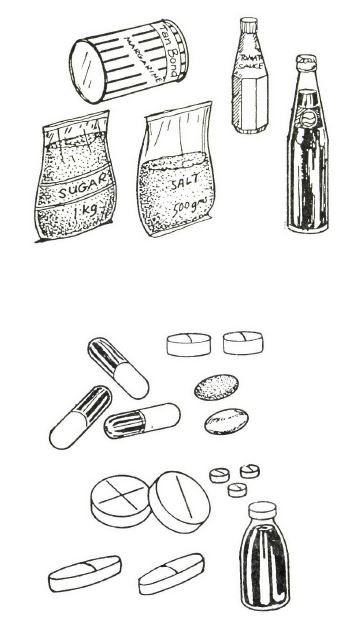
\includegraphics[width=0.45\textwidth]{./img/source/chemical-products.jpg}
\end{center}

\begin{description*}
%\item[Subtopic:]{}
%\item[Materials:]{}
%\item[Setup:]{}
\item[Procedure:]{In order to demonstrate the importance of
chemistry in daily life, ask the students to display
and label things produced by chemists. Ask
them to arrange similar products together.}
%\item[Hazards:]{}
%\item[Questions:]{}
%\item[Observations:]{}
%\item[Theory:]{}
%\item[Applications:]{}
%\item[Notes:]{}
\end{description*}

\columnbreak

During an introduction to chemistry students
should be shown where their lives and the
products they use link in with the chemical
industry.
Students' own experience of chemistry comes
from their daily lives and not from working in a
laboratory. A students environment is their
chemistry lab!

\subsection{Pollution and Chemistry}

\begin{center}
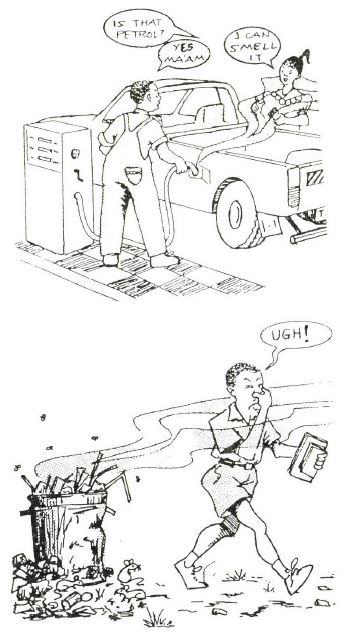
\includegraphics[width=0.45\textwidth]{./img/source/chemical-pollution.jpg}
\end{center}

\begin{description*}
%\item[Subtopic:]{}
%\item[Materials:]{}
%\item[Setup:]{}
\item[Procedure:]{In order to build up an awareness of pollution
in our environment, let the students describe
some situations where pollution of air, water
and soil happen.}
%\item[Hazards:]{}
\item[Questions:]{What can be done to reduce these forms of pollution?}
%\item[Observations:]{}
%\item[Theory:]{}
%\item[Applications:]{}
%\item[Notes:]{}
\end{description*}

\subsection{Making an Excursion}

\begin{center}
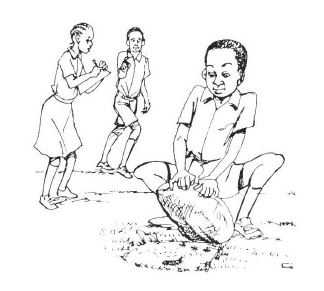
\includegraphics[width=0.45\textwidth]{./img/source/excursion.jpg}
\end{center}

\begin{description*}
%\item[Subtopic:]{}
%\item[Materials:]{}
%\item[Setup:]{}
\item[Procedure:]{It can be stimulating to make an excursion
around the school ground, to find out where
chemical processes can be observed. There can
be natural ones like the decomposition of organic
substances, cooking, alcoholic drink
production, etc.}
%\item[Hazards:]{}
%\item[Questions:]{}
%\item[Observations:]{}
%\item[Theory:]{}
%\item[Applications:]{}
%\item[Notes:]{}
\end{description*}

\subsection{Posters of Chemical Products}

\begin{center}
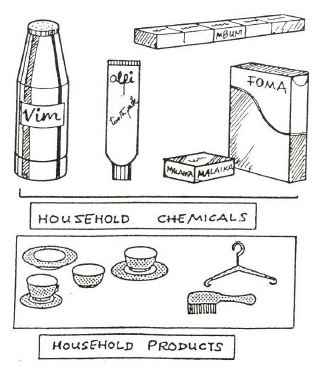
\includegraphics[width=0.45\textwidth]{./img/source/chemical-posters.jpg}
\end{center}

\begin{description*}
%\item[Subtopic:]{}
\item[Materials:]{Manila paper, marker pens, newspapers, scissors}
%\item[Setup:]{}
\item[Procedure:]{Instead of displaying real products, posters
can be made in groups with pictures cut out
from newspapers. For language training let the
pupils talk about their work and what the posters
show.}
%\item[Hazards:]{}
%\item[Questions:]{}
%\item[Observations:]{}
%\item[Theory:]{}
%\item[Applications:]{}
%\item[Notes:]{}
\end{description*}

\subsection{We Are All Chemists}

\begin{center}
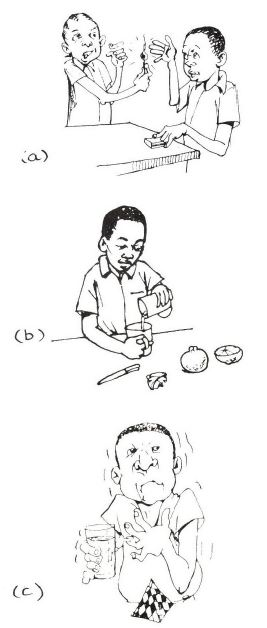
\includegraphics[width=0.45\textwidth]{./img/source/all-chemists.jpg}
\end{center}

\begin{description*}
%\item[Subtopic:]{}
%\item[Materials:]{}
%\item[Setup:]{}
\item[Procedure:]{Students should understand that we are all
chemists and not only those people working in
a chemical lab. Let them try out examples of
chemical processes with locally available
materials.
\begin{itemize}
\item[(a)] Carefully burn some paper, wood, fuel or
ignite a matchstick.
\item[(b)] Add some lemon juice to a cup of tea and
observe the colour change.
\item[(c)] Let a glass of milk go sour.
\item[(d)] Rub some red or pink petals from flowers on
wet soap firmly and observe the change of the
colour.
\item[(e)] Try to find some more examples.
\end{itemize}
}
%\item[Hazards:]{}
%\item[Questions:]{}
%\item[Observations:]{}
%\item[Theory:]{}
%\item[Applications:]{}
%\item[Notes:]{}
\end{description*}

%==================================================================================================%


\end{multicols}

\pagebreak
%\section{Laboratory Techniques and Safety}

\begin{multicols}{2}


%\section*{}


\subsection{Display of Hazardous \hfill \\ Chemicals}

\begin{center}
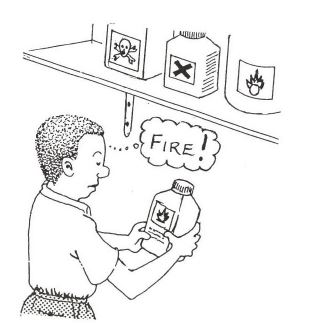
\includegraphics[width=0.45\textwidth]{./img/source/display-chemicals.jpg}
\end{center}

\begin{description*}
%\item[Subtopic:]{}
%\item[Materials:]{}
%\item[Setup:]{}
\item[Procedure:]{Display some well labelled containers with
hazard symbols for the students and let them
talk about them.}
%\item[Hazards:]{}
%\item[Questions:]{}
%\item[Observations:]{}
%\item[Theory:]{}
%\item[Applications:]{}
%\item[Notes:]{}
\end{description*}

\subsection{A Safety Game}

\begin{center}
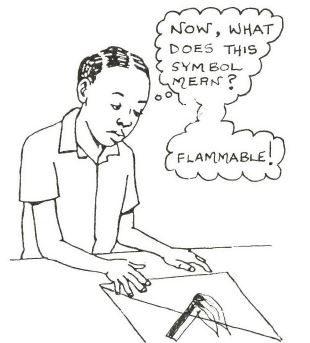
\includegraphics[width=0.45\textwidth]{./img/source/safety-game.jpg}
\end{center}

\begin{description*}
%\item[Subtopic:]{}
\item[Materials:]{Cards of hazard symbols}
%\item[Setup:]{}
\item[Procedure:]{Play a game with the symbol charts. A
student is given a hazard symbol. He has to
explain the hazard shown and to explain the
necessary safety precautions in order to avoid
that hazard.}
%\item[Hazards:]{}
%\item[Questions:]{}
%\item[Observations:]{}
%\item[Theory:]{}
%\item[Applications:]{}
%\item[Notes:]{}
\end{description*}

\columnbreak

\subsection{The Cleanliness Play}

\begin{center}

\includegraphics[width=0.45\textwidth]{./img/source/cleanliness-play.jpg}
\end{center}

\begin{description*}
%\item[Subtopic:]{}
%\item[Materials:]{}
%\item[Setup:]{}
\item[Procedure:]{Ask the students to play group-wise short
and funny scenes using appropriate words to
make them familiar with cleanliness rules.}
%\item[Hazards:]{}
%\item[Questions:]{}
%\item[Observations:]{}
%\item[Theory:]{}
%\item[Applications:]{}
%\item[Notes:]{}
\end{description*}

\subsection{The Tidiness Play}

\begin{center}
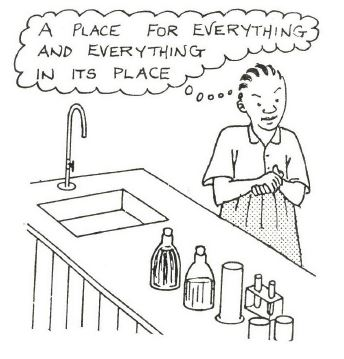
\includegraphics[width=0.45\textwidth]{./img/source/tidiness-play.jpg}
\end{center}

\begin{description*}
%\item[Subtopic:]{}
%\item[Materials:]{}
%\item[Setup:]{}
\item[Procedure:]{Chemists are very tidy. Apparatus and
reagents should be arranged on the table so that
they can be reached easily but at a safe distance
from the experiment.}
%\item[Hazards:]{}
%\item[Questions:]{}
%\item[Observations:]{}
%\item[Theory:]{}
%\item[Applications:]{}
%\item[Notes:]{}
\end{description*}

%==================================================================================================%


\end{multicols}

\pagebreak
%\section{Heat Sources and Flames} \index{Heat sources}

\begin{multicols}{2}


\section*{Heat Sources}


\begin{description*}
%\item[Subtopic:]{}
\item[Materials:]{Candle, bottle cap, kerosene burner, tin cans, wire, charcoal, glass jar, metal tubes}
%\item[Setup:]{}
\item[Procedure:]{Construct the simple heat sources shown below.}
%\item[Hazards:]{}
\item[Questions:]{What are the advantages and disadvantages of each?}
%\item[Observations:]{}
%\item[Theory:]{}
%\item[Applications:]{}
%\item[Notes:]{}
\end{description*}

\subsection{Candle Burner} \index{Candle burner}

\begin{center}
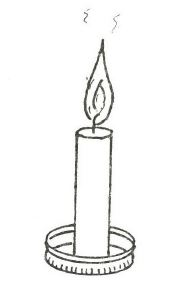
\includegraphics[width=0.1\textwidth]{./img/source/candle-burner.jpg}
\end{center}

\subsection{Kerosene Burner} \index{Kerosene burner}

\begin{center}
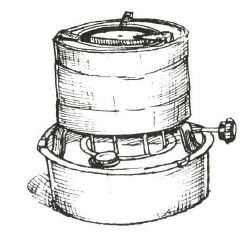
\includegraphics[width=0.3\textwidth]{./img/source/kerosene-burner.jpg}
\end{center}

\subsection{Spirit Burner} \index{Spirit burner}

\begin{center}
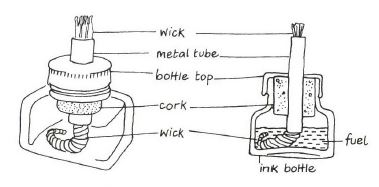
\includegraphics[width=0.49\textwidth]{./img/vso/spirit-burner.jpg}
\end{center}

\subsection{Charcoal Burner} \index{Charcoal burner}

\begin{center}
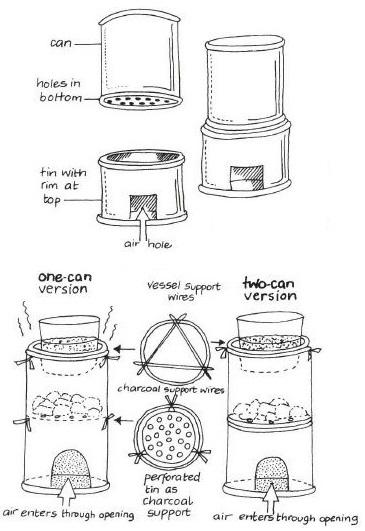
\includegraphics[width=0.49\textwidth]{./img/vso/charcoal-burner.jpg}
\end{center}

\subsection{Types of Flames} \index{Flames}

%\begin{center}
%\includegraphics[width=0.4\textwidth]{./img/.png}
%\end{center}

\begin{description*}
%\item[Subtopic:]{}
\item[Materials:]{Kerosene burner, candle, methylated spirit, kerosene, motopoa, bottle caps, matches, spoon, paper, metal jar lid}
%\item[Setup:]{}
\item[Procedure:]{Light a kerosene burner and observe the flame, adjusting the height of the wicks. Light small amounts of methylated spirit and motopoa in separate bottle caps. Light the candle and observe the flame. Light the paper on a metal lid and observe the flame. For each test, hold a metal spoon over the flame and examine for soot.}
%\item[Hazards:]{}
%\item[Questions:]{}
\item[Observations:]{Kerosene produces a luminous flame. A long wick gives a bigger and brighter flame with more soot. Spirit and motopoa produce non-luminous flames and does not produce soot. Candles and burning paper produce a luminous flame and deposit soot on the spoon.}
%\item[Theory:]{}
%\item[Applications:]{}
%\item[Notes:]{}
\end{description*}


%==================================================================================================%


\end{multicols}

\pagebreak
%\section{The Scientific Procedure}

%\begin{multicols}{2}


\section{Chemistry}


\subsection{Acids and Bases}

\begin{center}
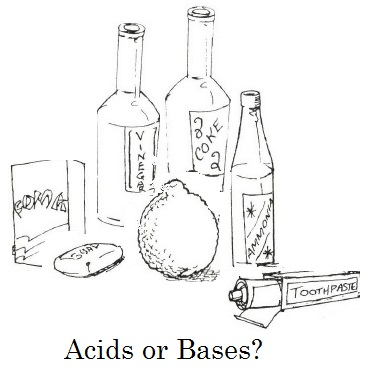
\includegraphics[width=0.4\textwidth]{./img/source/acids-bases-sci-meth.jpg}
\end{center}

\begin{description*}
\item[Materials:]{Bottles, bottle caps, water, vinegar, lemons, baking soda, soda, soap, antacid tablets, rosella leaves, straws/syringes}
\item[Setup:]{Prepare solutions for each of the items above in separate bottles. Prepare indicator by placing rosella leaves in hot water.}\\
\item[Problem:]{What differences can we observe among acids and bases?\\

\begin{tabular}{|l|c|c|} \hline
\multirow{2}{*}{\textbf{Solutions}} & \textbf{Hypothesis} & \multirow{2}{*}{\textbf{Experimental Result}} \\
& \textbf{(Which is different?)} & \\ \hline
Vinegar, lemon, baking soda & & \\ \hline
Vinegar, baking soda, soap & & \\ \hline
Baking soda, antacid, soda & & \\ \hline
Soda, soap, vinegar & & \\ \hline
\end{tabular} \\[10pt]
}
\item[Hypothesis:]{For each set of solutions, which one will reveal a colour different from the others? Record your predictions in the table.}
\item[Procedure:]{Place small amounts of 3 different solutions in separate bottle caps according to the table. Add a few drops of rosella indicator to each.}
\item[Observations:]{Record observations of colour change under \emph{Experimental Result} in the table.}
\item[Questions:]{\hfill
\begin{enumerate}
\item Which solutions have similar properties?
\item Which solutions are acids? What colour do they show?
\item Which solutions are bases? What colour do they show?
\end{enumerate}
}
\item[Theory:]{Coloured leaves such as rosella act as indicators for identifying acids and bases. Adding rosella indicator reveals a red colour for acids and a blue colour for bases. Students do not need to understand the differences between acids and bases in order to observe their different behaviours. Locally available examples of acids include sour milk, citrus fruits and soda. Local bases include ammonia, toothpaste and detergent.}
\end{description*}


\subsection{Mixing Acids and Bases}

\begin{center}
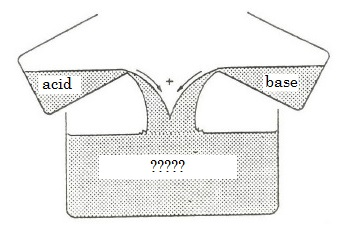
\includegraphics[width=0.6\textwidth]{./img/source/mixing-acid-base.jpg}
\end{center}

\begin{description*}
\item[Problem:]{What happens when acids and bases are mixed together?\\

\begin{tabular}{|l|c|c|} \hline
\multirow{2}{*}{\textbf{Solutions to Mix}} & \textbf{Hypothesis} & \multirow{2}{*}{\textbf{Experimental Result}} \\
& \textbf{(What colour?)} & \\ \hline
Mix vinegar and lemon & & \\ \hline
Mix baking soda and soap & & \\ \hline
Mix vinegar and baking soda & & \\ \hline
\end{tabular}\\[10pt]
}
\item[Hypothesis:]{Predict any colour changes or observations when pairs of solutions are mixed together. Record in the table.}
\item[Procedure:]{Mix small amounts of solutions together according to the table.}
\item[Observations:]{Record observations (colour changes, etc.) in the table.}
\item[Questions:]{\hfill
\begin{enumerate}
\item What happens when an acid is mixed with an acid?
\item What happens when a base is mixed with a base?
\item What happens when an acid is mixed with a base?
\end{enumerate}
}
\item[Theory:]{Mixing acids with acids and bases with bases may cause the colour of the solution to turn darker or lighter depending on the solutions used. Mixing an acid with a base should reveal a colourless solution and produce carbon dioxide gas. You may need to vary the amounts of acid and base to get a colourless solution depending on their concentrations.}
\end{description*}

%==================================================================================================%


%\end{multicols}

\pagebreak
%\section{Matter}

\begin{multicols}{2}


\section*{Concept of Matter}


\subsection{Air is Matter}

\begin{center}
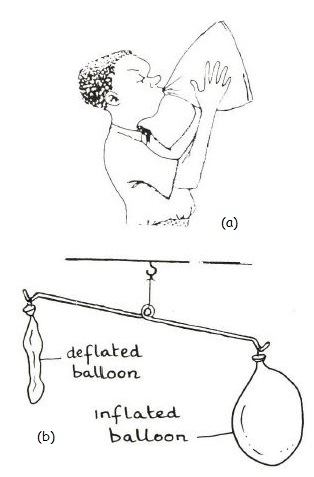
\includegraphics[width=0.4\textwidth]{./img/source/air-matter.jpg}
\end{center}

\begin{description*}
%\item[Subtopic:]{}
%\item[Materials:]{Balloons/plastic bags, wire}
%\item[Setup:]{}
\item[Procedure:]{Blow a bag or balloon up with air (a). Hang a deflated bag and an inflated bag on either side of a simple wire balance.}
%\item[Hazards:]{}
%\item[Questions:]{}
\item[Observations:]{Air in the bag occupies space. The air has mass as indicated by the balance.}
%\item[Theory:]{}
%\item[Applications:]{}
%\item[Notes:]{}
\end{description*}

\subsection{Liquid is Matter}

\begin{center}
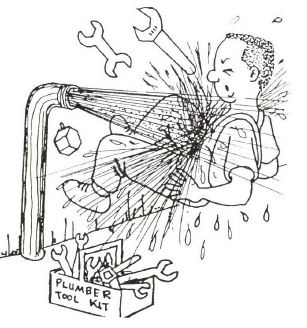
\includegraphics[width=0.4\textwidth]{./img/source/liquid-matter.jpg}
\end{center}

\begin{description*}
%\item[Subtopic:]{}
%\item[Materials:]{}
%\item[Setup:]{}
%\item[Procedure:]{}
%\item[Hazards:]{}
%\item[Questions:]{}
%\item[Observations:]{}
\item[Theory:]{Liquids contain mass, occupy space and can provide a great force under pressure. Don't be like the plumber in the picture!}
%\item[Applications:]{}
%\item[Notes:]{}
\end{description*}

%==================================================================================================%

\section*{States of Matter}
%All matter is made up of particles. These particles are in constant motion which increases with their temperature. Depending on temperature, matter may exist in three states: \emph{solid}, \emph{liquid} or \emph{gas}.
%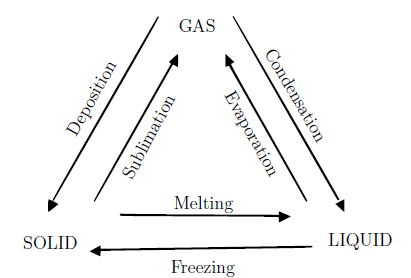
\includegraphics[width=0.4\textwidth]{./img/changes-of-state.png}

\subsection{Students as Matter}

\begin{center}
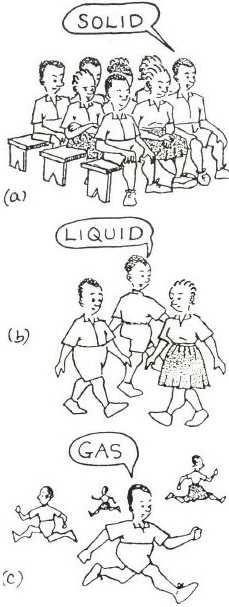
\includegraphics[width=0.35\textwidth]{./img/source/states-matter-students.jpg}
%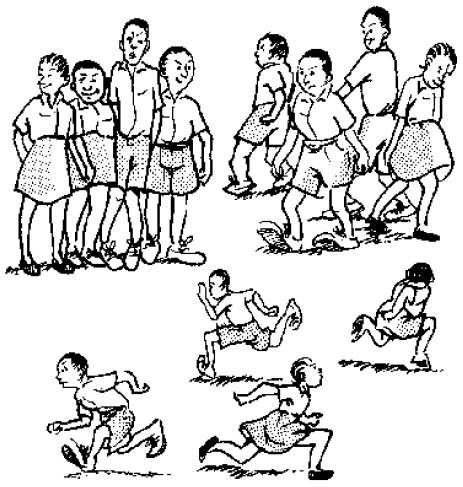
\includegraphics[width=0.4\textwidth]{./img/vso/states-matter.png}
\end{center}

\begin{description*}
%\item[Subtopic:]{}
%\item[Materials:]{}
%\item[Setup:]{}
\item[Procedure:]{Use students to demonstrate the concept of states of matter.}
%\item[Hazards:]{}
%\item[Questions:]{}
%\item[Observations:]{}
\item[Theory:]{When students or objects are close together, they represent particles in the \emph{solid} state. As they move apart and past each other they represent particles in the \emph{liquid} state. Fast and randomly moving pupils or objects represent particles in the \emph{gaseous} state.}
%\item[Applications:]{}
%\item[Notes:]{}
\end{description*}

\subsection{Arranging States of Matter}

\begin{center}
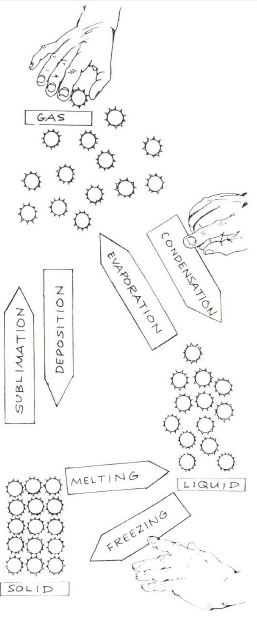
\includegraphics[width=0.4\textwidth]{./img/source/state-arranging.jpg}
\end{center}

\begin{description*}
%\item[Subtopic:]{}
\item[Materials:]{Bottle caps, paper}
%\item[Setup:]{}
\item[Procedure:]{Have students arrange bottle caps to represent the different states of matter, using labels from paper or cardboard.}
%\item[Hazards:]{}
%\item[Questions:]{}
%\item[Observations:]{}
\item[Theory:]{The spacing of the bottle caps represents the distance between particles in each state. Particles have large spaces between them in gases, less space in liquids, and are very condensed in solids.}
%\item[Applications:]{}
%\item[Notes:]{}
\end{description*}

\columnbreak

\subsection{A Model of Motion}

\begin{center}
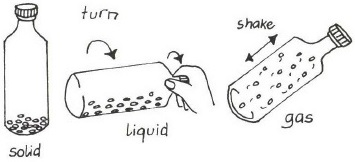
\includegraphics[width=0.49\textwidth]{./img/vso/motion-model.jpg}
\end{center}

\begin{description*}
%\item[Subtopic:]{}
%\item[Materials:]{}
%\item[Setup:]{}
\item[Procedure:]{Put some dry beans, rice or stones in a clear bottle. Hold the bottle still, then turn it, then shake it vigorously.}
%\item[Hazards:]{}
\item[Questions:]{Which activity corresponds to which state of matter?}
%\item[Observations:]{}
\item[Theory:]{The movement of particles in solids is small and hence they are in fixed order. In liquids the particles move past each other and have lost the stiff order. In gases they move very fast and randomly, losing all order.}
%\item[Applications:]{}
%\item[Notes:]{}
\end{description*}

%==================================================================================================%

\section*{Physical and Chemical Changes}


\subsection{Physical or Chemical?}

\begin{center}
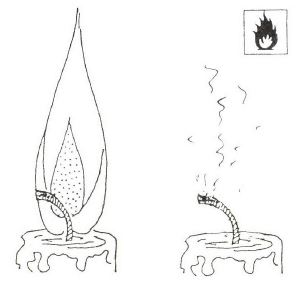
\includegraphics[width=0.35\textwidth]{./img/source/physical-change.jpg}
\end{center}

\begin{description*}
%\item[Subtopic:]{}
\item[Materials:]{Candle, paper, sugar, bottle caps}
%\item[Setup:]{}
\item[Procedure:]{Light a candle and let it drip into a bottle cap. Then light the paper and catch the remains in another cap. Finally place a small amount of sugar in a cap and heat it over the flame.}
%\item[Hazards:]{}
%\item[Questions:]{}
\item[Observations:]{The candle wax melts into a liquid, then upon cooling reforms into a solid. The paper burns up and leaves ash. The sugar turns brown upon heating, leaving a brownish black solid upon cooling.}
\item[Theory:]{The candle wax undergoes a physical change that only affects its physical properties. After heating, we can get the original wax back again by cooling. The paper and sugar undergo chemical changes since the change is not reversible.}
%\item[Applications:]{}
%\item[Notes:]{}
\end{description*}

\subsection[Physical and Chemical Changes of Metals]{Physical and Chemical \hfill \\ Changes of Metals}

\begin{center}
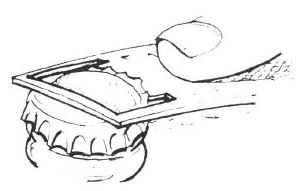
\includegraphics[width=0.4\textwidth]{./img/source/p-c-changes-metals.jpg}
\end{center}

\begin{description*}
%\item[Subtopic:]{}
\item[Materials:]{Soda bottle, various metals, \nameref{sec:heatsources}}
%\item[Setup:]{}
\item[Procedure:]{Physical and chemical changes can be
demonstrated with iron wool, copper, aluminium
or lead.

(a) Apply physical forces.

(b) Heat the metals in a strong flame (blow pipe
flame). Allow the metals to cool.}
%\item[Hazards:]{}
%\item[Questions:]{}
%\item[Observations:]{}
\item[Theory:]{If only the form has changed, these are
physical changes. If colour, density etc. have
changed permanently, these are chemical
changes.}
%\item[Applications:]{}
%\item[Notes:]{}
\end{description*}

%==================================================================================================%

\section*{Elements and Symbols}


\subsection{Element Memory Game} % PIC!!!

%\begin{center}
%\includegraphics[width=0.4\textwidth]{./img/.jpg}
%\end{center}

\begin{description*}
%\item[Subtopic:]{}
\item[Materials:]{Manila paper/card/paper}
\item[Setup:]{Cut out 2 sets of identical small squares of card or paper. On the first set write the names of some elements and on the second set write their corresponding symbols. Make about 10-15 pairs. }
\item[Procedure:]{Mix the cards together and spread them out on a table face down. Students take turns flipping over 2 cards at a time. If the element and symbol match, they get to keep the cards. If not, they must turn them back over. The player with the most pairs of cards at the end wins!}
%\item[Hazards:]{}
%\item[Questions:]{}
%\item[Observations:]{}
%\item[Theory:]{}
%\item[Applications:]{}
%\item[Notes:]{}
\end{description*}

\vfill
\columnbreak

%==================================================================================================%

\section*{Compounds and Mixtures}


\subsection{Introducing Mixtures}

\begin{center}
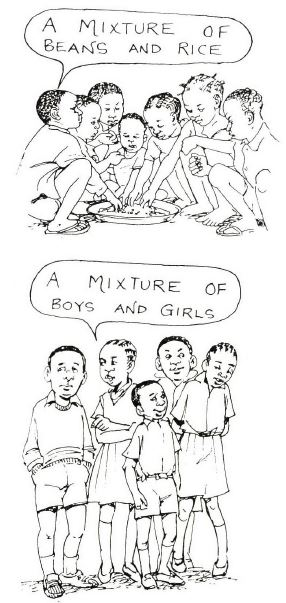
\includegraphics[width=0.45\textwidth]{./img/source/intro-mixtures.jpg}
\end{center}

\begin{description*}
%\item[Subtopic:]{}
%\item[Materials:]{}
%\item[Setup:]{}
\item[Procedure:]{Why not introduce mixrures with a
game? Students will like a more concrete
introduction. Try it!}
%\item[Hazards:]{}
%\item[Questions:]{}
%\item[Observations:]{}
%\item[Theory:]{}
%\item[Applications:]{}
%\item[Notes:]{}
\end{description*}

\vfill
\columnbreak

\subsection{Mixtures and Compounds}

\begin{center}
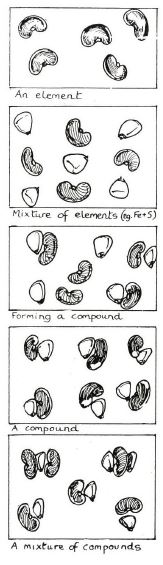
\includegraphics[width=0.3\textwidth]{./img/source/mixtures-compounds.jpg}
\end{center}

\begin{description*}
%\item[Subtopic:]{}
\item[Materials:]{Beans, seeds, corn kernels, etc.}
%\item[Setup:]{}
\item[Procedure:]{Use the items to represent various elements, mixtures and compounds as shown.}
%\item[Hazards:]{}
%\item[Questions:]{}
%\item[Observations:]{}
\item[Theory:]{In homogeneous mixtures, the particles are
uniformly mixed and it is impossible to see the
different ingredients even by using a light
microscope. For example, solutions and the
mixture of gases in air are homogeneous
mixtures.

In heterogeneous mixtures, the particles are
also uniformly mixed. But the individual
components can be seen either by eye or by
using a magnifying glass or microscope.}
%\item[Applications:]{}
%\item[Notes:]{}
\end{description*}

\subsection{Student Compounds}

\begin{center}
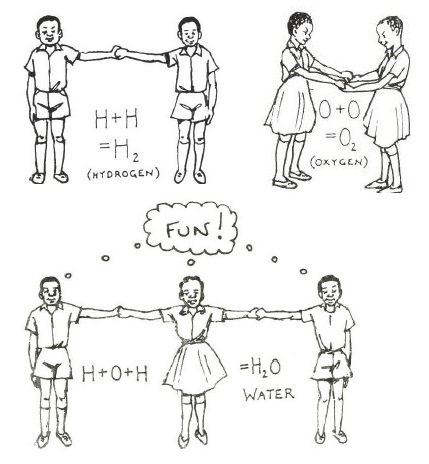
\includegraphics[width=0.45\textwidth]{./img/source/student-compounds.jpg}
\end{center}

\begin{description*}
%\item[Subtopic:]{}
%\item[Materials:]{}
%\item[Setup:]{}
\item[Procedure:]{To show that elements combine in constant
proportions, ask the students to play a game of
forming molecules like those of water, ammonia,
methane, ethane, carbon dioxide etc. See the
figures.}
%\item[Hazards:]{}
%\item[Questions:]{}
%\item[Observations:]{}
%\item[Theory:]{}
%\item[Applications:]{}
%\item[Notes:]{}
\end{description*}

\subsection{Homogeneous Mixtures}

\begin{center}
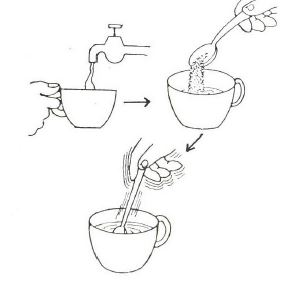
\includegraphics[width=0.4\textwidth]{./img/source/homogeneous.jpg}
\end{center}

\begin{description*}
%\item[Subtopic:]{}
\item[Materials:]{Salt, water, spoon, bottle}
%\item[Setup:]{}
\item[Procedure:]{Dissolve some table salt or sugar in drinking
water to demonstrate a solution as a
homogeneous mixture. Ask the pupils to taste
the solution to prove that the chemical properties
of the solute have not changed.}
\item[Hazards:]{Ensure that clean water, cups and spoons
are used.}
%\item[Questions:]{}
%\item[Observations:]{}
%\item[Theory:]{}
%\item[Applications:]{}
%\item[Notes:]{}
\end{description*}

\subsection{Heterogeneous Mixtures}

\begin{center}
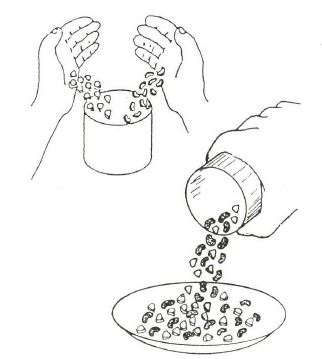
\includegraphics[width=0.4\textwidth]{./img/source/heterogeneous.jpg}
\end{center}

\begin{description*}
%\item[Subtopic:]{}
\item[Materials:]{Bean seeds, maize grains, salt, sand, sugar}
%\item[Setup:]{}
\item[Procedure:]{(a) Take a handful of maize grains and
another handful of bean seeds. Each handful is
like a pure substance having only one kind of
particle. Now mix the maize grains and the
beans in a container. 
Repeat with sand and salt or sand and sugar.}
%\item[Hazards:]{}
%\item[Questions:]{}
%\item[Observations:]{}
\item[Theory:]{This is like a heterogeneous
mixture since different particles can be seen.}
\item[Applications:]{Common everyday examples of
heterogenous mixtures are turbid water and
porridge. Preparing concrete is another example which can be observed in daily life.}
%\item[Notes:]{}
\end{description*}

\subsection{Separating Iron and Sulphur} % VSO 63

\begin{center}
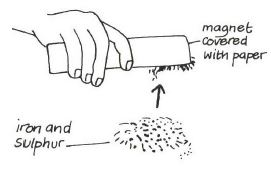
\includegraphics[width=0.4\textwidth]{./img/vso/iron-sulphur.jpg}
\end{center}

\begin{description*}
%\item[Subtopic:]{}
\item[Materials:]{Steel wool, sulphur powder, magnet, paper}
\item[Setup:]{Prepare a mixture of iron filings and sulphur powder.}
\item[Procedure:]{Cover the magnet with paper.
The magnet will attract only the
iron, leaving sulphur behind.}
%\item[Hazards:]{}
%\item[Questions:]{}
%\item[Observations:]{}
\item[Theory:]{The magnetic properties of the iron filings allow the magnet to separate the mixture by attracting the iron.}
%\item[Applications:]{}
%\item[Notes:]{}
\end{description*}

%\subsection{Types of Solutions} % PIC!!! Shika 296
%
%%\begin{center}
%%\includegraphics[width=0.4\textwidth]{./img/.jpg}
%%\end{center}
%
%\begin{description*}
%%\item[Subtopic:]{}
%\item[Materials:]{3 cups, water, salt, spoon}
%%\item[Setup:]{}
%\item[Procedure:]{Fill 3 cups with water. In the first add a bit of salt. In the second, add salt unitl it no longer dissolves. In the third, add salt until a small mound forms on the bottom. Stir each solution and taste a small amount.}
%%\item[Hazards:]{}
%%\item[Questions:]{}
%\item[Observations:]{Cup 1 tastes slightly salty, while cups 2 and 3 taste the same - very salty.}
%\item[Theory:]{Cup 1 contains an \emph{unsaturated} solution, i.e. it can still dissolve more salt. Cup 2 has a \emph{saturated} solution - it can dissolve no more salt. Cup 3 has a \emph{supersaturated} solution - it holds more undissolved salt at the bottom.}
%%\item[Applications:]{}
%%\item[Notes:]{}
%\end{description*}

%\subsection{Solutions, Suspensions and Emulsions} % LASM 48
%
%%\begin{center}
%%\includegraphics[width=0.4\textwidth]{./img/.jpg}
%%\end{center}
%
%\begin{description*}
%%\item[Subtopic:]{}
%\item[Materials:]{}
%\item[Setup:]{}
%\item[Procedure:]{}
%\item[Hazards:]{}
%\item[Questions:]{}
%\item[Observations:]{}
%\item[Theory:]{}
%\item[Applications:]{}
%\item[Notes:]{}
%\end{description*}

\subsection{Suspensions}

\begin{center}
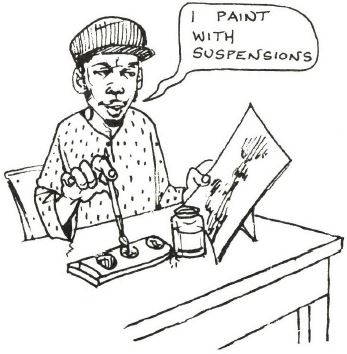
\includegraphics[width=0.4\textwidth]{./img/source/suspensions.jpg}
\end{center}

\begin{description*}
%\item[Subtopic:]{}
%\item[Materials:]{}
%\item[Setup:]{}
%\item[Procedure:]{}
%\item[Hazards:]{}
%\item[Questions:]{}
%\item[Observations:]{}
\item[Theory:]{A suspension is a mixture of a solid and a
liquid. Suspensions can be made from solids
like sand, soil, ash, sawdust etc. with a liquid
like water. }
\item[Applications:]{Let the students find more examples
from their daily life (e.g. toothpaste and
porridge).}
%\item[Notes:]{}
\end{description*}

\subsection{Emulsions} % Source 93, Shika 288

\begin{center}
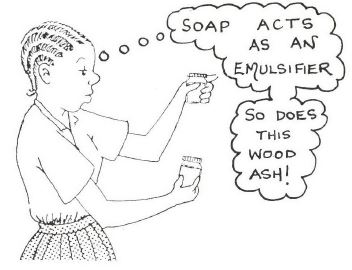
\includegraphics[width=0.4\textwidth]{./img/source/emulsions.jpg}
\end{center}

\begin{description*}
%\item[Subtopic:]{}
\item[Materials:]{Kerosene/oil, water, bottle, soap}
%\item[Setup:]{}
%\item[Procedure:]{}
%\item[Hazards:]{}
%\item[Questions:]{}
%\item[Observations:]{}
\item[Theory:]{Emulsions are made from two immiscible
liquids like kerosene or oil in water. Shake and
let it stand for some time to demonstrate an
unstable emulsion. If soap is added to the water
it acts as an emulsifier and stabilizes the
emulsion. Wood ash also acts in this way. }
\item[Applications:]{Let the students find more examples in
daily life (e.g. milk).}
%\item[Notes:]{}
\end{description*}

\subsection[Miscible and Immiscible Liquids]{Miscible and Immiscible \hfill \\ Liquids} % Source 93, Shika 287

\begin{center}
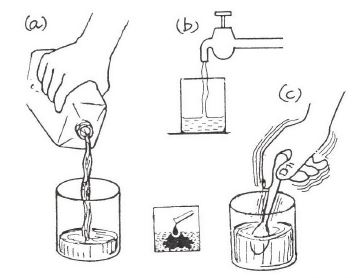
\includegraphics[width=0.4\textwidth]{./img/source/miscible-immiscible.jpg}
\end{center}

\begin{description*}
%\item[Subtopic:]{}
\item[Materials:]{Water, kerosene, alcohol, bottles}
%\item[Setup:]{}
\item[Procedure:]{Mix equal amounts of water separately with
kerosene and alcohol in two different containers.}
\item[Hazards:]{Kerosene is water polluting! Do not pour it
into the sink. Keep it in a labeled container for
further experiments.}
%\item[Questions:]{}
%\item[Observations:]{}
\item[Theory:]{The water and kerosene combine to make an immiscible liquid, whereas the water and alcohol form a miscible liquid.}
%\item[Applications:]{}
%\item[Notes:]{}
\end{description*}

\subsection{Lava Lamp} % PIC!!! Shika 286

%\begin{center}
%\includegraphics[width=0.4\textwidth]{./img/.jpg}
%\end{center}

\begin{description*}
%\item[Subtopic:]{}
\item[Materials:]{Bottle, water, food coloring, oil, effervescing
antacid tablets, 
ashlight,}
%\item[Setup:]{}
\item[Procedure:]{Fill the bottom 10 cm of a water bottle with water. Add
a few drops of food coloring. Fill rest of the bottle with oil. Drop in
an effervescing antacid tablet. Cap and put a 
flashlight underneath the
bottle. }
%\item[Hazards:]{}
%\item[Questions:]{}
\item[Observations:]{Observe the colors and the movement of the liquids.}
\item[Theory:]{Oil is a compound that is hydrophobic (it repels
water). Oil is a long non-polar hydrocarbon, while water
is a small polar compound. This means that the water cannot mix with
the oil layer. This is why there are two layers on mixing oil and water.
Adding the effervescing antacid tablets dissolve and release carbon dioxide
in the water layer. The carbon dioxide dissolves in the water and forms
small bubbles of carbon dioxide. These bubbles trap small amounts of
food coloring. These bubbles rise since they have a much lower density
than water. When the bubble reaches the surface, the carbon dioxide
escapes and the colored water bubble falls down through the oil layer.}
%\item[Applications:]{}
%\item[Notes:]{}
\end{description*}

\columnbreak

\subsection{Moving Colours} % PIC!!! Shika 286

%\begin{center}
%\includegraphics[width=0.4\textwidth]{./img/.jpg}
%\end{center}

\begin{description*}
%\item[Subtopic:]{}
\item[Materials:]{Milk, various food colouring, powdered soap, cotton ball or swab, shallow dish or plate}
%\item[Setup:]{}
\item[Procedure:]{Pour in just enough milk to cover the plate or the bowl. Place a few drops of
food colouring around the plate of milk. Soak
the cotton swab in some soapy water and touch it to the center of the
milk plate. }
%\item[Hazards:]{}
%\item[Questions:]{}
\item[Observations:]{The colours will start to move and
swirl towards the center.}
\item[Theory:]{Milk is made up of fats and different proteins (non-polar molecules). The water solution in the food colour and the non polar milk barely mix. Soap
is a compound that is both polar on one end and non polar on the other
end. The milk and the soap intermingle forming micelles. In addition,
the surface tension of the water in the milk breaks, allowing
food colouring to move around in the milk. }
%\item[Applications:]{}
%\item[Notes:]{}
\end{description*}

%==================================================================================================%

\section*{Separating Mixtures}


\subsection{Decantation}

\begin{center}
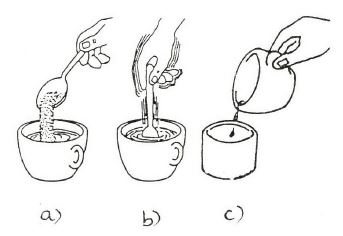
\includegraphics[width=0.4\textwidth]{./img/source/decantation.jpg}
\end{center}

\begin{description*}
%\item[Subtopic:]{}
\item[Materials:]{Cup, water, sand}
%\item[Setup:]{}
\item[Procedure:]{This procedure is based on the different
density of particles.
Shake some sand with water, let it stand for
some time and decant the water.}
%\item[Hazards:]{}
%\item[Questions:]{}
%\item[Observations:]{}
%\item[Theory:]{}
\item[Applications:]{Maize seeds are usually washed before milling.
After washing the maize seeds are separated
from the water by decantation.}
%\item[Notes:]{}
\end{description*}

\columnbreak

\subsection{Evaporation}

\begin{center}
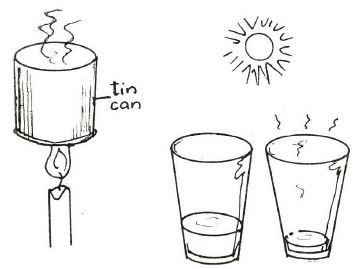
\includegraphics[width=0.4\textwidth]{./img/source/evaporation.jpg}
\end{center}

\begin{description*}
%\item[Subtopic:]{}
\item[Materials:]{Container, salt, water}
%\item[Setup:]{}
\item[Procedure:]{This procedure is based on different
boiling points.
(a) Dissolve some common salt in water and
heat to dryness.
(b) Better crystals can be obtained by evaporating
most of the water. The remaining water can be
evaporated slowly in the sun.}
%\item[Hazards:]{}
%\item[Questions:]{}
%\item[Observations:]{}
%\item[Theory:]{}
%\item[Applications:]{}
%\item[Notes:]{}
\end{description*}

\subsection{Distillation}

\begin{center}
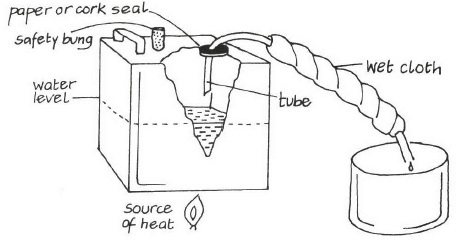
\includegraphics[width=0.49\textwidth]{./img/vso/distillation.jpg}
\end{center}

\begin{description*}
%\item[Subtopic:]{}
\item[Materials:]{Metal can, cork/rubber stopper, plastic tubing, wet cloth, container, \nameref{sec:heatsources}}
%\item[Setup:]{}
\item[Procedure:]{Fill a container half way with water. Cut a hole in the top and fix a rubber stopper with a plastic tube through the center. Wrap a wet cloth around the tube and feed it into a can. Add a safety bung using rubber or cork to prevent against very high pressures within the container and place the container over the heat source.}
\item[Hazards:]{Make sure the safety bung is not too tight and that the container always has water inside.}
%\item[Questions:]{}
%\item[Observations:]{}
\item[Theory:]{Heating the can produces steam which is then cooled by the wet cloth. Steam condenses to produce water.}
\item[Applications:]{This method can be used to purify water.}
%\item[Notes:]{}
\end{description*}

\columnbreak

\subsection{Distillation of a Solution}

\begin{center}
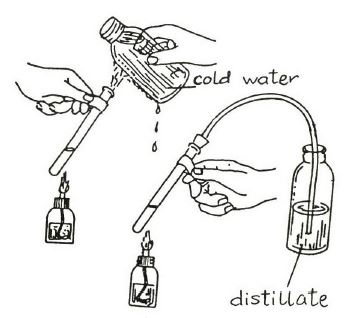
\includegraphics[width=0.4\textwidth]{./img/source/distillation-solution.jpg}
\end{center}

\begin{description*}
%\item[Subtopic:]{}
\item[Materials:]{Candle, bottles, cold water, ash extract, tube}
%\item[Setup:]{}
\item[Procedure:]{Take the ash extract obtained by filtration and distill it as shown. The
ash extract is separated into a liquid (distillate)
and a solid residue.}
\item[Hazards:]{Take care due to the small diameter of the
connection tubes.}
%\item[Questions:]{}
%\item[Observations:]{}
\item[Theory:]{The solids have a much higher boiling point
than the water.}
%\item[Applications:]{}
%\item[Notes:]{}
\end{description*}

\subsection[Separating Immiscible Liquids]{Separating Immiscible \hfill \\ Liquids} % VSO 63

\begin{center}
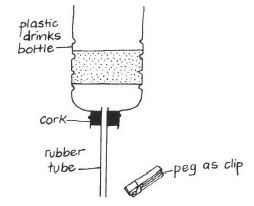
\includegraphics[width=0.4\textwidth]{./img/vso/sep-immiscible.jpg}
\end{center}

\begin{description*}
%\item[Subtopic:]{}
\item[Materials:]{Kerosene, water, bottle, cork, rubber tube, clothespin}
%\item[Setup:]{}
\item[Procedure:]{Combine 2 liquids together that do not mix well, e.g. groundnut oil and water; palm oil
and water; petrol/diesel and
water; castor oil and water. Palm
oil is particularly effective because
it is brightly coloured.}
%\item[Hazards:]{}
%\item[Questions:]{}
%\item[Observations:]{}
\item[Theory:]{When 2 liquids will not mix with
each other they are said to be
immiscible. One liquid will sink
below the other and can be
drawn off as shown.}
%\item[Applications:]{}
%\item[Notes:]{}
\end{description*}

\columnbreak

\subsection{Filtration}

\begin{center}
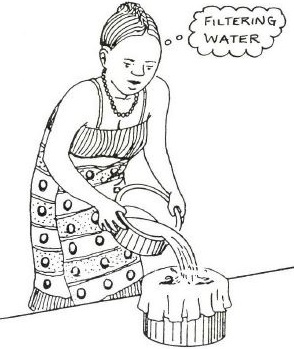
\includegraphics[width=0.35\textwidth]{./img/source/filtering-2.jpg}
\end{center}

\begin{description*}
%\item[Subtopic:]{}
%\item[Materials:]{}
%\item[Setup:]{}
%\item[Procedure:]{}
%\item[Hazards:]{}
%\item[Questions:]{}
%\item[Observations:]{}
\item[Theory:]{Filtering is based on the same principle as
sieving. It is a frequently used process in daily
life. The students can explain different filtering
processes they know.}
%\item[Applications:]{}
%\item[Notes:]{}
\end{description*}

\subsection{Chromatography} % Source 97, LASM 56, Shika 247

\begin{center}
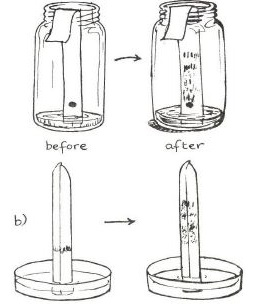
\includegraphics[width=0.4\textwidth]{./img/source/chromatography-2.jpg} 
\end{center}

\begin{description*}
%\item[Subtopic:]{}
\item[Materials:]{Pen/marker, newspaper, water, chalk, ink}
%\item[Setup:]{}
\item[Procedure:]{(a) Make a line with ink or a black felt pen (containing water soluble
colour) on a strip made from filter paper or the white rim of a newspaper. Hang the strip into
water, so that the spot is above the water level.

(b) Stand a piece of chalk in ink. The chalk must
stand upright.}
%\item[Hazards:]{}
%\item[Questions:]{}
%\item[Observations:]{}
\item[Theory:]{This procedure is based on the differeni
capillary rise of soluble substances in a porous
support. Many colours are mixtures. The different
colours rise at different speeds and thus separate.}
%\item[Applications:]{}
%\item[Notes:]{}
\end{description*}

%==================================================================================================%


\end{multicols}

\pagebreak
%\section{Air, Combustion, Rusting and Fire Fighting}

\begin{multicols}{2}

\section*{Composition of Air}


\subsection{What is Air?}

\begin{center}
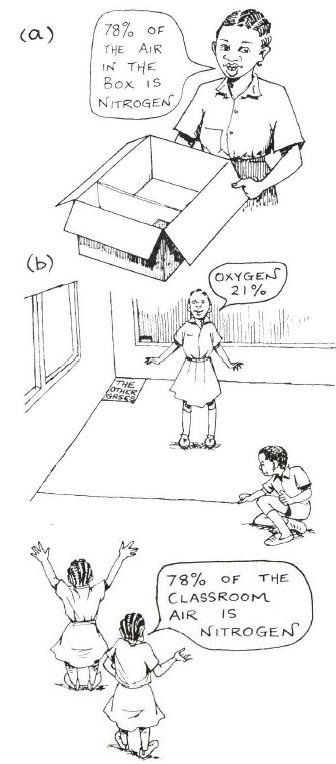
\includegraphics[width=0.45\textwidth]{./img/source/air-comp-1.jpg}
\end{center}

\begin{description*}
%\item[Subtopic:]{}
%\item[Materials:]{}
%\item[Setup:]{}
\item[Procedure:]{(a) To show the percentage by volume of
the different gases in air take a cardboard box of
about 50 cm $\times$ 50 cm $\times$ 50 cm and partition it
using cardboard pieces as shown in diagram (a)
according to the following figures: Nitrogen
78\%, Oxygen 2l\%, other 1\% (Argon 0.93\%,
other noble gases 0.002\%, carbon dioxide 0.03\%,
hydrogen 0.00l\%).
(b) The classroom can be imagined to be a box
with a certain volume of air and divided
accordingly by students as shown.}
%\item[Hazards:]{}
%\item[Questions:]{}
%\item[Observations:]{}
%\item[Theory:]{}
%\item[Applications:]{}
%\item[Notes:]{}
\end{description*}

\subsection{Gases in Air}

\begin{center}
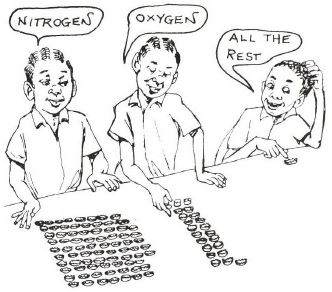
\includegraphics[width=0.4\textwidth]{./img/source/gases-in-air.jpg}
\end{center}

\begin{description*}
%\item[Subtopic:]{}
\item[Materials:]{Bottle tops/stones}
%\item[Setup:]{}
\item[Procedure:]{Collect a hundred bottle tops or
stones. Arrange in ten rows of ten. Each bottle
top represents one percent (by volume) of the
gases in the air. The bottle tops can then be
divided according to the percentages described
in the previous activity.}
%\item[Hazards:]{}
%\item[Questions:]{}
%\item[Observations:]{}
%\item[Theory:]{}
%\item[Applications:]{}
%\item[Notes:]{}
\end{description*}

%==================================================================================================%

\section*{Combustion}


\subsection{Requirements for Combustion}

\begin{center}
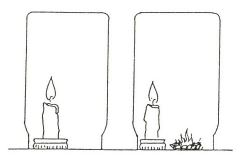
\includegraphics[width=0.4\textwidth]{./img/source/flame-extinguisher.jpg}
\end{center}

\begin{description*}
%\item[Subtopic:]{}
\item[Materials:]{2 glass jars, 2 candles, bottle caps, kerosene or spirit}
%\item[Setup:]{}
\item[Procedure:]{Place 1 jar over a lit candle and the other jar over both a candle and a kerosene or spirit flame in a bottle cap.}
%\item[Hazards:]{}
\item[Questions:]{Which candle flame goes out first?}
\item[Observations:]{The candle in the jar with the spirit burner goes out first.}
\item[Theory:]{Three elements are necessary for combustion: heat, fuel and oxygen. In the second jar, both the candle and spirit flame are consuming oxygen and so the oxygen gets depleted faster, extinguishing the flame.}
%\item[Applications:]{}
%\item[Notes:]{}
\end{description*}

\subsection{Rising Water}

\begin{center}
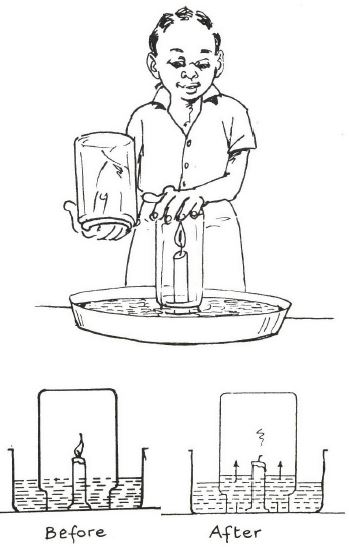
\includegraphics[width=0.4\textwidth]{./img/source/candle-water.jpg}
\end{center}

\begin{description*}
%\item[Subtopic:]{}
\item[Materials:]{Candle, dish, water, glass}
%\item[Setup:]{}
\item[Procedure:]{Place a candle in a dish fixing it securely with
melted wax. Fill the dish with water. Put glasses
of different sizes over the candle.}
%\item[Hazards:]{}
%\item[Questions:]{}
\item[Observations:]{The water rises to different levels after the flame goes out.}
\item[Theory:]{Once the glass is placed over the candle, the flame consumes the remainder of the oxygen in the glass, replacing it with carbon dioxide and other gases. The heating of the gases causes expansion and bubbles come out of the jar. This is followed by their subsequent cooling and contraction, which reduces the volume of gas inside the glass and allows water to enter.}
%\item[Applications:]{}
%\item[Notes:]{}
\end{description*}

\subsection{\texorpdfstring{\ce{H_2O}}{H_2O} as a Product of \hfill \\ Combustion} % Pic from elsewhere??? condensation

%\begin{center}
%\includegraphics[width=0.4\textwidth]{./img/.jpg}
%\end{center}

\begin{description*}
%\item[Subtopic:]{}
\item[Materials:]{Glass jar/plastic bottle, water, candle}
%\item[Setup:]{}
\item[Procedure:]{Fill the bottle with water and hold it just above a lit candle, far enough so that it does not burn.}
%\item[Hazards:]{}
%\item[Questions:]{}
\item[Observations:]{After a minute or two, condensation forms on the outside of the container, showing that water is a product of combustion.}
%\item[Theory:]{}
%\item[Applications:]{}
%\item[Notes:]{}
\end{description*}

\columnbreak

\subsection{\texorpdfstring{\ce{CO_2}}{CO_2} as a Product of \hfill \\ Combustion}

\begin{center}
\includegraphics[width=0.4\textwidth]{./img/source/co2-extinguisher.jpg}
\end{center}

\begin{description*}
%\item[Subtopic:]{}
\item[Materials:]{Tall glass, wood ash, dilute acid, match, candle}
%\item[Setup:]{}
\item[Procedure:]{Place some wood ash in a tall glass and add some dilute acid. Drop a lit match into the glass and wait for it to stop burning. Now pour the glass over a lit candle.}
%\item[Hazards:]{}
%\item[Questions:]{}
\item[Observations:]{Pouring the glass puts out the candle flame.}
\item[Theory:]{The carbon dioxide produced stays in the
glass since it is denser than air. Carbon dioxide
extinguishes flames since it does not support
combustion.}
\item[Applications:]{Fire extinguishers}
%\item[Notes:]{}
\end{description*}

\subsection{Burning Money}

%\begin{center}
%\includegraphics[width=0.4\textwidth]{./img/.jpg}
%\end{center}

\begin{description*}
%\item[Subtopic:]{}
\item[Materials:]{Methylated spirits, water, container, matches, paper money, clothespin}
%\item[Setup:]{}
\item[Procedure:]{Make a mixture of 3 parts methylated spirits and 2 parts water. Soak the money in the mixture. Remove with a clothespin and light it with a match. After about 5 seconds drop the money into the extra water.}
%\item[Hazards:]{}
%\item[Questions:]{}
\item[Observations:]{The money appears to burn but remains intact.}
\item[Theory:]{The ethanol in the methylated spirit burns at a low temperature while the water protects the bill from combusting. However, if there is a lot of ethanol and it burns for a long time, the water will evaporate away and the bill will start burning.}
%\item[Applications:]{}
%\item[Notes:]{}
\end{description*}

%==================================================================================================%

\section*{Firefighting}


\subsection{Putting Out Fires} % LASM 37

\begin{center}
\includegraphics[width=0.4\textwidth]{./img/source/fire-fighting.jpg}
\end{center}

\begin{description*}
%\item[Subtopic:]{}
\item[Materials:]{Bottle caps, ethanol, kerosene, water, matches, sand, glass jar}
%\item[Setup:]{}
\item[Procedure:]{Put a small amount of ethanol into a bottle cap and light it with a match. Pour water onto the flame. Repeat using a handful of sand and then an inverted glass over the flame. Now add a small amount of kerosene to a bottle cap. Repeat the above methods, but add water \emph{carefully} using a syringe near the base of the flame. Repeat the steps for a burning piece of paper.}
\item[Hazards:]{Perform these tests on a laboratory floor, not a wooden table or desk.}
%\item[Questions:]{}
\item[Observations:]{The ethanol and paper flames are extinguished in all 3 cases. However, adding water to the kerosene \emph{does not} extinguish it.}
\item[Theory:]{Overturning a glass jar deprives the flames of oxygen and thus extinguishes them. A kerosene fire can NOT be extinguished by water because water is immiscible with kerosene, and it only causes the fire to spread.}
%\item[Applications:]{}
%\item[Notes:]{}
\end{description*}

\vfill
\columnbreak

\subsection{Making a Fire Extinguisher}

\begin{center}
\includegraphics[width=0.35\textwidth]{./img/fire-extinguisher.jpg}
\end{center}

\begin{description*}
%\item[Subtopic:]{}
\item[Materials:]{Bottle, tea bag, bicarbonate of soda, vinegar, water, plastic tube, super glue}
\item[Setup:]{Empty a tea bag and fill it with sodium bicarbonate. Suspend it in a bottle half-filled with a vinegar-water solution. Poke a hole in the cap and insert a plastic tube. Make sure it is sealed using super glue or clay.}
\item[Procedure:]{Invert the bottle and use the tube to direct the spray at a lit candle.}
%\item[Hazards:]{}
%\item[Questions:]{}
%\item[Observations:]{}
\item[Theory:]{The reaction produces carbon dioxide gas which extinguishes flames. This is how fire extinguishers eliminate flames.}
%\item[Applications:]{}
%\item[Notes:]{}
\end{description*}

\vfill
\columnbreak

%==================================================================================================%

\section*{Rusting}


\subsection{Conditions for Rusting}

\begin{center}
\includegraphics[width=0.4\textwidth]{./img/rusting-nails-6.png}
\end{center}

\begin{description*}
%\item[Subtopic:]{}
\item[Materials:]{6 syringes, 6 nails, water, oil, paint}
\item[Setup:]{Seal the bottoms of the syringes by melting the plastic.}
\item[Procedure:]{Place a nail in each syringe. Paint the final nail. Fill the syringes as shown, closing some of them with their plungers. Observe the nails over time and note which ones show rusting.}
%\item[Hazards:]{}
%\item[Questions:]{}
\item[Observations:]{Syringe 1 should show rusting, while the others do not.}
\item[Theory:]{Syringe 1 is the control - both water and oxygen react with the nail. In syringe 2, no oxygen is available. In syringe 3, there is no water and oil makes it difficult for oxygen to reach the nail. In syringe 4, neither water nor oxygen are present. In syringe 5, water is available, but the layer of oil prevents oxygen from reaching it since oxygen does not travel easily through oil. In syringe 6, painting covers the iron surface, so there is no iron to produce rusting.}
%\item[Applications:]{}
%\item[Notes:]{}
\end{description*}

\subsection{Rusting of Steel Wool} % VSO 65

\begin{center}
\includegraphics[width=0.35\textwidth]{./img/vso/rusting-steel-wool.jpg}
\end{center}

\begin{description*}
%\item[Subtopic:]{}
\item[Materials:]{Steel wool, candle, 2 glass containers}
%\item[Setup:]{}
\item[Procedure:]{Wet the steel wool and place some in each container. Seal one
container. Place a lighted candle in the other container. When the
candle has burnt for several minutes seal the container with a lid. The
candle will go out eventually. Leave both containers for 2 days. }
%\item[Hazards:]{}
%\item[Questions:]{}
\item[Observations:]{The
steel wool in the container with the candle should not rust as much
because oxygen has been removed by the candle.}
%\item[Theory:]{}
%\item[Applications:]{}
%\item[Notes:]{}
\end{description*}

\columnbreak

\subsection{Rusty Nails}

\begin{center}
\includegraphics[width=0.4\textwidth]{./img/vso/rusty-nails.jpg}
\end{center}

\begin{description*}
%\item[Subtopic:]{}
\item[Materials:]{3 containers, 2 nails, boiled water, tap water}
%\item[Setup:]{}
\item[Procedure:]{Place a nail in each of the
containers and leave for a day.}
%\item[Hazards:]{}
%\item[Questions:]{}
\item[Observations:]{The only nail which does not rust
is the one in the sealed jar of
boiled water.}
\item[Theory:]{Boiling the water
removes the oxygen and sealing it
prevents oxygen from the air
dissolving in it.}
%\item[Applications:]{}
%\item[Notes:]{}
\end{description*}

\subsection{Preventing Rusting} % VSO 65

\begin{center}
\includegraphics[width=0.4\textwidth]{./img/source/rusting-prevent.jpg}
\end{center}

\begin{description*}
%\item[Subtopic:]{}
\item[Materials:]{tin can, oil}
%\item[Setup:]{}
\item[Procedure:]{Make 2 large scratches on the surface of a tin can (not an aluminium
can often used for drinks). Put a thin layer of oil onto one scratch.
Leave the tin exposed to the air for a few days. Note which scratch
rusts.}
%\item[Hazards:]{}
%\item[Questions:]{}
\item[Observations:]{The scratch not covered in oil rusts, while the other does not.}
\item[Theory:]{Oil prevents water and oxygen from reaching the surface of metal, and so no rusting occurs.}
\item[Applications:]{Machine parts often cannot be protected by painting or other means so they are regularly oiled.}
%\item[Notes:]{}
\end{description*}

%==================================================================================================%


\end{multicols}

\pagebreak

% Form II
\chapter{Chemistry Activities for Form II}
%\section{Oxygen}

\begin{multicols}{2}


\section*{Preparation of Oxygen}


\subsection{Using Hydrogen Peroxide}

%\begin{center}
%\includegraphics[width=0.4\textwidth]{./img/.png}
%\end{center}

\begin{description*}
%\item[Subtopic:]{}
\item[Materials:]{Dry cell, hydrogen peroxide, water, plastic bottle}
\item[Setup:]{Open a dry cell battery and peel back the metal casing to reveal a black powder. This is Manganese (IV) oxide. }
\item[Procedure:]{Scoop out the powder and place in a plastic bottle. Add about 20 mL of dilute hydrogen peroxide. Crush and cap the bottle.}
\item[Hazards:]{Hydrogen peroxide is corrosive. Be sure to dilute the solution.}
%\item[Questions:]{}
\item[Observations:]{The bottle inflates with oxygen gas.}
\item[Theory:]{Hydrogen peroxide decomposes into water and oxygen rather easily. The manganese (IV) dioxide acts as a catalyst. The chemical equation for this reaction is: \[ 2\mathrm{H}_2\mathrm{O}_2 + ( \mathrm{Mn}\mathrm{O}_2 ) \longrightarrow 2\mathrm{H}_2\mathrm{O} + \mathrm{O}_2 \]}
%\item[Applications:]{}
%\item[Notes:]{}
\end{description*}

\subsection{Using A Yeast Catalyst} % Shika 229

%\begin{center}
%\includegraphics[width=0.4\textwidth]{./img/.jpg}
%\end{center}

\begin{description*}
%\item[Subtopic:]{}
\item[Materials:]{Hydrogen peroxide, water, yeast, plastic bottle}
%\item[Setup:]{}
\item[Procedure:]{Place a small amount of dilute hydrogen peroxide in a plastic bottle. Crush the bottle and add some yeast. Cap the bottle and gently invert.}
%\item[Hazards:]{}
%\item[Questions:]{}
%\item[Observations:]{}
\item[Theory:]{Yeast contains an enzyme called catalase, which helps to break down hydrogen peroxide into oxygen and water. The enzyme protects the organism by eating the peroxide.}
%\item[Applications:]{}
%\item[Notes:]{}
\end{description*}

\subsection{Elephant Toothpaste} % PIC!!!

%\begin{center}
%\includegraphics[width=0.4\textwidth]{./img/.jpg}
%\end{center}

\begin{description*}
%\item[Subtopic:]{}
\item[Materials:]{Syringe/measuring cylinder, powdered soap, yeast, hydrogen peroxide, food colour}
%\item[Setup:]{}
\item[Procedure:]{Mix powdered soap and a warm yeast solution in a syringe or large measuring cylinder. Add food colouring if desired. Pour in hydrogen peroxide.}
%\item[Hazards:]{}
%\item[Questions:]{}
\item[Observations:]{A large amount of foam/bubbles bursts out of the container.}
\item[Theory:]{Catalase decomposes hydrogen peroxide to form water and oxygen
gas. The soap
traps the gas in bubbles. These bubbles build up upon each other, slowly
forcing them out of the container. }
%\item[Applications:]{}
%\item[Notes:]{}
\end{description*}

\vfill
\columnbreak

\subsection{Using Potassium Manganate (VII)} % Shika 282

\begin{center}
\includegraphics[width=0.25\textwidth]{./img/source/oxygen-prep.jpg}
\end{center}

\begin{description*}
%\item[Subtopic:]{}
\item[Materials:]{Potassium manganate (VII), \nameref{sec:heatsources}, test tube/light bulb}
%\item[Setup:]{}
\item[Procedure:]{Carefully heat potassium manganate (VII) (permanganate) in a test
tube or in an opened electric bulb.}
%\item[Hazards:]{}
%\item[Questions:]{}
%\item[Observations:]{}
\item[Theory:]{Chemical equation for this reaction: \[ 2\mathrm{K}\mathrm{Mn}\mathrm{O}_4 \longrightarrow \mathrm{K}_2\mathrm{Mn}\mathrm{O}_4 + \mathrm{Mn}\mathrm{O}_2 + \mathrm{O}_2 \]}
%\item[Applications:]{}
%\item[Notes:]{}
\end{description*}

%==================================================================================================%

\section*{Properties of Oxygen}


\subsection{Burning in Pure Oxygen}

\begin{center}
\includegraphics[width=0.4\textwidth]{./img/source/burning-oxygen.jpg}
\end{center}

\begin{description*}
%\item[Subtopic:]{}
\item[Materials:]{Charcoal, deflagrating spoon, straw, bottle}
%\item[Setup:]{}
\item[Procedure:]{(a) Ignite charcoal in a deflagrating spoon
using a blow pipe. Then put the deflagrating
spoon with the burning charcoal into a glass full
of pure oxygen.

(b) Bring glowing iron wool into a glass full of
pure oxygen.}
%\item[Hazards:]{}
%\item[Questions:]{}
\item[Observations:]{Both substances bum with bright flame.}
\item[Theory:]{Charcoal forms carbon dioxide and iron
forms iron oxide. Both reactions give out heat
(exothermic reactions).}
%\item[Applications:]{}
%\item[Notes:]{}
\end{description*}

%==================================================================================================%


\end{multicols}

\pagebreak
%\section{Hydrogen}

\begin{multicols}{2}


\section*{}


\subsection{}

\begin{center}
\includegraphics[width=0.4\textwidth]{./img/.png}
\end{center}

\begin{description*}
%\item[Subtopic:]{}
\item[Materials:]{}
\item[Setup:]{}
\item[Procedure:]{}
\item[Hazards:]{}
\item[Questions:]{}
\item[Observations:]{}
\item[Theory:]{}
\item[Applications:]{}
\item[Notes:]{}
\end{description*}

%==================================================================================================%


\end{multicols}

\pagebreak
%\section{Water} \index{Water|textbf}

\begin{multicols}{2}


\section*{Occurrence and Nature \hfill \\ of Water} \index{Water! occurrence and nature of}


\subsection{The Water Cycle} \index{Water! cycle}

\begin{center}
\includegraphics[width=0.4\textwidth]{./img/source/water-cycle.jpg}
\end{center}

\begin{description*}
%\item[Subtopic:]{}
\item[Materials:]{Cards, scissors}
%\item[Setup:]{}
\item[Procedure:]{Cut out cards and label them according to different terms associated with the water cycle (e.g. evaporation, condensation, precipitation, transpiration, collection). Sketch the picture shown and have students label where each takes place.}
%\item[Hazards:]{}
%\item[Questions:]{}
%\item[Observations:]{}
%\item[Theory:]{}
%\item[Applications:]{}
%\item[Notes:]{}
\end{description*}

\subsection{Cloud in a Jar} \index{Clouds}

%\begin{center}
%\includegraphics[width=0.4\textwidth]{./img/.jpg}
%\end{center}

\begin{description*}
%\item[Subtopic:]{}
\item[Materials:]{Wide mouth glass jar, balloon/latex glove, water, matches}
%\item[Setup:]{}
\item[Procedure:]{Add a small amount of water to the jar. Stretch the mouth of the balloon around the mouth of the jar and insert it so it hangs in the bottle. Pull the balloon out and quickly open the seal and drop in a lit match. Quickly reseal, pushing the balloon back inside the bottle, and then pull the balloon outside of the jar again.}
%\item[Hazards:]{}
%\item[Questions:]{}
\item[Observations:]{A cloud forms inside the jar.}
\item[Theory:]{By putting the balloon in the jar and pulling it out, the volume inside the container increases and some of the water turns into vapour. Dropping a match creates smoke and other particles where rain can form. Pulling the balloon out again lowers the temperature by decreasing the volume enough to start forming clouds.}
\item[Applications:]{Clouds in the sky are formed when water vapour is cooled to form tiny water droplets.}
%\item[Notes:]{}
\end{description*}

%==================================================================================================%

\section*{Properties of Water} \index{Water! properties of}


\subsection{Test for Water} % LASM 76 PIC!!!

%\begin{center}
%\includegraphics[width=0.4\textwidth]{./img/.jpg}
%\end{center}

\begin{description*}
%\item[Subtopic:]{}
\item[Materials:]{Copper (II) sulphate, spoon, candle, water}
%\item[Setup:]{}
\item[Procedure:]{Place a small amount of blue copper (II) sulphate in a metal spoon. Heat the spoon over the candle until the crystals have changed from blue to white. Add a few drops of water to the white crystals. }
%\item[Hazards:]{}
%\item[Questions:]{}
%\item[Observations:]{}
\item[Theory:]{On heating blue hydrated copper (II) sulphate, the colour changes from blue
($\mathrm{Cu}\mathrm{SO}_4\cdot 5\mathrm{H}_2\mathrm{O}$) to white ($\mathrm{Cu}\mathrm{SO}_4$). On addition of a few drops of water $\mathrm{Cu}\mathrm{SO}_4$ returns to its original hydrated state (blue), i.e. copper sulphate pentahydrated.}
%\item[Applications:]{}
%\item[Notes:]{}
\end{description*}

%==================================================================================================%

\section*{Importance of Water}


\subsection{Wasted Water}

\begin{center}
\includegraphics[width=0.4\textwidth]{./img/source/water-waste.jpg}
\end{center}

\begin{description*}
%\item[Subtopic:]{}
%\item[Materials:]{}
%\item[Setup:]{}
\item[Procedure:]{Conduct an experiment or survey at your school or village. If you have a dripping tap or leaking pipe, try to find out how much water it wastes each day. Collect the water and measure the volume lost over 15 minutes and then calculate how much would be lost in a day, week, etc.}
%\item[Hazards:]{}
%\item[Questions:]{}
%\item[Observations:]{}
%\item[Theory:]{}
\item[Applications:]{Water is essential for all life. Many areas have very little access to water. What can you do in your community to reduce water waste?}
%\item[Notes:]{}
\end{description*}

\columnbreak

\subsection{Water in Daily Life}

\begin{center}
\includegraphics[width=0.4\textwidth]{./img/source/water-daily-life.jpg}
\end{center}

\begin{description*}
%\item[Subtopic:]{}
%\item[Materials:]{}
%\item[Setup:]{}
\item[Procedure:]{Ask the students to
talk about:

(a) The importance of water in daily life;

(b) Where and why water is being polluted;

(c) How contaminated water may harm people.}
%\item[Hazards:]{}
%\item[Questions:]{}
%\item[Observations:]{}
\item[Theory:]{(b) People washing or urinating in/near
rivers, lakes; used lubricating oil of cars etc.
being dumped on soil may enter the ground
water table; factories using chemicals (e.g.
tanneries, paper mills, fertilizer plants, pesticide
plants etc.) may pollute rivers, lakes etc.

(c) People may get typhoid fever, cholera etc.
when drinking contaminated water from rivers,
lakes or wells; water contaminated by factories
may cause cancer etc.}
%\item[Applications:]{}
%\item[Notes:]{}
\end{description*}

%==================================================================================================%

\section*{Treatment and Purification of Water} \index{Water! treatment of}


\subsection{The `SODIS' Method} \index{SODIS} % PIC!!!

%\begin{center}
%\includegraphics[width=0.4\textwidth]{./img/.jpg}
%\end{center}

\begin{description*}
%\item[Subtopic:]{}
%\item[Materials:]{}
%\item[Setup:]{}
\item[Procedure:]{Fill a bottle with water from a tap. Place it on the roof of your house in open sunlight for 2 days or 3-4 days if it is cloudy. Filter through a clean cloth or kanga.}
%\item[Hazards:]{}
%\item[Questions:]{}
%\item[Observations:]{}
\item[Theory:]{Ultraviolet rays from the sun kill the harmful bacteria in the water that cause disease. Filtering though a cloth removes solid impurities.}
%\item[Applications:]{}
%\item[Notes:]{}
\end{description*}

\columnbreak

\subsection{Constructing a Water Filter} \index{Filtration}

\begin{center}
\includegraphics[width=0.4\textwidth]{./img/water-filter.png}
\end{center}

\begin{description*}
%\item[Subtopic:]{}
\item[Materials:]{Fine sand, coarse sand, small pebbles, large pebbles, charcoal, empty bottle, dirty water}
\item[Setup:]{Rinse off all pebbles and remove and dirt from the sand. Cut the bottom of a bottle so it is shaped like a funnel.}
\item[Procedure:]{Invert the bottle and place the large pebbles, followed by smaller pebbles, coarse sand, charcoal and sand on top. Run water through until it comes out clean on bottom.}
%\item[Hazards:]{}
%\item[Questions:]{}
%\item[Observations:]{}
\item[Theory:]{When dirty water passes through sand particles, impurities are trapped and
remain above. The smallest particles and some micro-organisms are stopped
by the charcoal layer.}
%\item[Applications:]{}
%\item[Notes:]{}
\end{description*}

%\vfill
%\columnbreak

\subsection{Water Treatment at Home}

%\begin{center}
%\includegraphics[width=0.4\textwidth]{./img/.jpg}
%\end{center}

\begin{description*}
%\item[Subtopic:]{}
\item[Materials:]{\nameref{sec:heatsources}, pot, water, clean cloth, bucket}
%\item[Setup:]{}
\item[Procedure:]{Boil a pot of water and let it cool. Then pour through a clean cloth or kanga into a clean bucket. The water is now safe for drinking.}
%\item[Hazards:]{}
%\item[Questions:]{}
%\item[Observations:]{}
\item[Theory:]{Boiling water at the boiling point (100$^\circ$C) kills the germs and
bacteria which may cause diseases. Filtration with a piece of clean white
cloth removes any solid impurities.}
%\item[Applications:]{}
%\item[Notes:]{}
\end{description*}

%==================================================================================================%


\end{multicols}

\pagebreak
%\section{Fuels and Energy}

\begin{multicols}{2}


\section*{Transformation of Energy}


\subsection{Chemical to Electrical Energy} % LASM

\begin{center}
\includegraphics[width=0.49\textwidth]{./img/source/chem-energy.jpg}
\end{center}

\begin{description*}
%\item[Subtopic:]{}
\item[Materials:]{Copper (II) sulphate, zinc metal (from dry cell), copper wire, steel wool, ammeter/bulb}
\item[Setup:]{Prepare a 2 M solution of copper (II) sulphate and clean pieces of copper wire and zinc using steel wool.}
\item[Procedure:]{Connect the zinc anode, ammeter/bulb and copper cathode in series using connecting wires. Dip the zinc and copper electrodes into the copper (II) sulphate solution. Read the current on the ammeter.}
%\item[Hazards:]{}
%\item[Questions:]{}
\item[Observations:]{The ammeter shows a deflection, possibly around 0.05 A.}
\item[Theory:]{The current produced indicates that the chemical energy inherent in the electrodes and the electrolyte solution is converted to electrical energy.}
%\item[Applications:]{}
%\item[Notes:]{}
\end{description*}

\vfill
\columnbreak

\subsection{Making an Electric Heater}

\begin{center}
\includegraphics[width=0.3\textwidth]{./img/electric-heater.png}
\end{center}

\begin{description*}
%\item[Subtopic:]{}
\item[Materials:]{Nichrome (resistance) wire (1 m), cardboard tube, speaker wire, 2-4 dry cells, water container, thermometer (optional)}
%\item[Setup:]{}
\item[Procedure:]{Coil the resistance wire around a cardboard tube so that the coils are close but not touching. Use speaker wires to connect the ends of the resistance wire to the terminals of the batteries. Place the coil of resistance wire into the container of water.}
\item[Hazards:]{Do not touch the water when current is flowing. If the heater is connected to the cells while not in the water, the wire can melt or burn other objects.}
%\item[Questions:]{}
\item[Observations:]{By touching the water container \emph{on the outside}, it begins to warm up. If left for long enough, the water will begin to boil.}
\item[Theory:]{The electric heater converts electrical energy into heat energy. The larger the coils are, the more efficient the heater will be.}
\item[Applications:]{Boiling water, heating houses}
%\item[Notes:]{}
\end{description*}

%\subsection{Wind Turbine}
%
%\begin{center}
%\includegraphics[width=0.4\textwidth]{./img/wind-turbine.png}
%\end{center}
%
%\begin{description*}
%%\item[Subtopic:]{}
%\item[Materials:]{30 cm $\times$ 30 cm flexible plastic sheet, pin, scissors, super glue, plastic water bottle, small motor (e.g. from car stereo), connecting wires, galvanometer}
%\item[Propeller:]{Make 5 small holes in the plastic sheet - one at each corner and one in the middle. Cut along the curved lines shown. Fold each corner towards the centre so that all five holes are aligned and glue them in place. Cut the top off of a water bottle just below the lip where the cap sits. Glue the bottle top to the propeller as shown. }
%\item[Generator:]{Make a small hole in the centre of the bottle cap using a pin. Glue the top of the cap to the motor wheel so that the two spin together evenly.}
%\item[Setup:]{Screw the propeller onto the generator like closing a bottle. The propeller should be able to turn freely on the motor. Connect the terminals of the motor to the terminals of the galvanometer.}
%\item[Procedure:]{Hold the propeller upright into the wind so that it spins.}
%%\item[Hazards:]{}
%%\item[Questions:]{}
%\item[Observations:]{The galvanometer will deflect to show that a current is being created in the wire.}
%\item[Theory:]{Mechanical energy (wind) is converted into electrical energy (electric current) using a generator.}
%%\item[Applications:]{Sustainable energy sources}
%%\item[Notes:]{}
%\end{description*}

\vfill
\columnbreak

\subsection{Water Turbine}

\begin{center}
\includegraphics[width=0.45\textwidth]{./img/water-turbine.png}
\end{center}

\begin{description*}
%\item[Subtopic:]{}
\item[Materials:]{Plastic bottle, small motor (e.g. from car stereo), super glue, \nameref{sec:heatsources}, heated nail or soldering iron, 9 water bottle caps, 8 syringe needle caps, scissors, water and pitcher, connecting wires, galvanometer}
\item[Water Wheel:]{Using a hot nail or soldering iron, melt the open end of a syringe needle cap to the side of a water bottle cap to create a sort of spoon. Repeat 7 more times for a total of 8 pieces. Cut the top off a water bottle just below the lip which holds the cap. Melt a plastic cap over the cut end of the bottle top so that the threaded side is open. Use the hot nail or soldering iron to melt 8 holes evenly around the side of this central bottle cap. Insert the 8 spokes into the holes so that they create an 8-spoke wheel with all of the cups facing in one direction at equal distances from the centre. Melt the plastic around each spoke to secure them in place.}
\item[Generator:]{Make a small hole in the centre of the bottle cap using a pin. Glue the top of the cap to the motor wheel so that the two spin together evenly.}
\item[Setup:]{Screw the water wheel onto the generator like closing a bottle. The water wheel should be able to turn freely on the motor. Connect the terminals of the motor to the terminals of the galvanometer.}
\item[Procedure:]{Pour water from a pitcher or spout and place the water wheel under the water so that it turns vertically.}
%\item[Hazards:]{}
%\item[Questions:]{}
\item[Observations:]{The galvanometer will deflect to show that a current is being created in the wire.}
\item[Theory:]{Mechanical energy (falling water and subsequent rotating water wheel) is converted into electrical energy (electric current) using a generator.}
%\item[Applications:]{Sustainable energy sources}
%\item[Notes:]{}
\end{description*}

%==================================================================================================%

%\section*{Energy Changes in Chemical Reactions}
%
%
%\subsection{Endothermic and Exothermic Reactions} % Alt = Chemical Kinetics
%
%\begin{center}
%\includegraphics[width=0.4\textwidth]{./img/source/exothermic.jpg}
%\end{center}
%
%\begin{description*}
%%\item[Subtopic:]{}
%\item[Materials:]{3 plastic bottles, powdered soap, citric acid, spoon}
%%\item[Setup:]{}
%\item[Procedure:]{Add a small amount of water to each bottle. Add 3 spoons of powdered laundry soap (e.g. Omo, Foma) to the first bottle. Add 3 spoons of citric acid to the second bottle and nothing to the third bottle. Shake each vigorously and feel to observe any changes in temperature.}
%%\item[Hazards:]{}
%%\item[Questions:]{}
%%\item[Observations:]{}
%\item[Theory:]{The dissolution of laundry soap in water is exothermic -- this bottle should
%get warmer. The dissolution of citric acid is endothermic -- this bottle should get cooler.}
%%\item[Applications:]{}
%%\item[Notes:]{}
%\end{description*}

%\subsection{Endothermic Reactions}
%
%%\begin{center}
%%\includegraphics[width=0.4\textwidth]{./img/.png}
%%\end{center}
%
%\begin{description*}
%%\item[Subtopic:]{}
%\item[Materials:]{Ammonium nitrate, water, container, thermometer (optional)}
%%\item[Setup:]{}
%\item[Procedure:]{Add water to a container or beaker. Add a small amount of ammonium nitrate and stir gently. After all of the ammonium nitrate has dissolved, feel the container or read the thermometer. }
%%\item[Hazards:]{}
%%\item[Questions:]{}
%\item[Observations:]{The container has cooled.}
%\item[Theory:]{This is an example of an \emph{endothermic} reaction. The heat content of the products is greater than the heat contents of the reactants, so the extra energy required is absorbed from the water.}
%%\item[Applications:]{}
%%\item[Notes:]{}
%\end{description*}
%
%\subsection{Exothermic Reactions}
%
%\begin{center}
%\includegraphics[width=0.4\textwidth]{./img/source/exothermic.jpg}
%\end{center}
%
%\begin{description*}
%%\item[Subtopic:]{}
%\item[Materials:]{Battery acid, sodium hydroxide, bottle, thermometer (optional)}
%%\item[Setup:]{}
%\item[Procedure:]{Add a small amount of water to the container. Carefully pour a small amount of battery acid down the side of the container using a syringe or test tube. Gently stir and \emph{carefully} touch the side of the container or read the thermometer.}
%\item[Hazards:]{The reaction between water and acid produces a lot of heat. Be extremely careful when touching the container. Do not use a highly concentrated acid and always wear goggles.}
%%\item[Questions:]{}
%\item[Observations:]{The container becomes very warm.}
%\item[Theory:]{This is an example of an \emph{exothermic} reaction. The total heat content of the reactants is greater than that of the products, so excess energy is lost to the water.}
%%\item[Applications:]{}
%%\item[Notes:]{}
%\end{description*}

\vfill
\columnbreak

%==================================================================================================%

\section*{Alternative Forms of Energy}


\subsection{Windmills}

\begin{center}
\includegraphics[width=0.35\textwidth]{./img/windmill.png}
\end{center}

\begin{description*}
%\item[Subtopic:]{}
\item[Materials:]{Paper/plastic sheet, scissors, pen, glue, paper fastener/thumb tack, straw or stick}
%\item[Setup:]{}
\item[Procedure:]{Copy the illustration onto a sheet of plastic or paper. Cut along the lines and make holes with a pen. Bend the four corners together into the center and glue them in place. Push the fastener through the center into a straw or stick.}
%\item[Hazards:]{}
%\item[Questions:]{}
%\item[Observations:]{}
%\item[Theory:]{}
%\item[Applications:]{Wind energy, wind turbines (see \nameref{sec:electromagnetism}.}
%\item[Notes:]{}
\end{description*}

%\subsection{Water Wheel}
%
%\begin{center}
%\includegraphics[width=0.5\textwidth]{./img/water-wheel.jpg}
%\end{center}
%
%\begin{description*}
%%\item[Subtopic:]{}
%\item[Materials:]{Stiff cardboard, scissors, nails, string, water, basin}
%\item[Setup:]{Construct the water wheel as shown.}
%\item[Procedure:]{Tie a small weight (e.g. paperclip, nail) to the string so that it rests on the floor. Pour water over the water wheel to turn it and lift the weight. }
%%\item[Hazards:]{}
%%\item[Questions:]{}
%%\item[Observations:]{}
%\item[Theory:]{Water stores potential energy in the forms of rivers and waterfalls and when placed in an elevated storage tank. The kinetic energy of falling water can be used to do work on an object and generate electricity.}
%\item[Applications:]{Water turbines (see \nameref{sec:electromagnetism} (p.~\pageref{sec:electromagnetism}).}
%%\item[Notes:]{}
%\end{description*}


%==================================================================================================%


\end{multicols}

\pagebreak
%\section{Atomic Structure}

\begin{multicols}{2}


\section*{}


\subsection{}

\begin{center}
\includegraphics[width=0.4\textwidth]{./img/.png}
\end{center}

\begin{description*}
%\item[Subtopic:]{}
\item[Materials:]{}
\item[Setup:]{}
\item[Procedure:]{}
\item[Hazards:]{}
\item[Questions:]{}
\item[Observations:]{}
\item[Theory:]{}
\item[Applications:]{}
\item[Notes:]{}
\end{description*}

%==================================================================================================%


\end{multicols}

\pagebreak
%\section{Periodic Classification}

\begin{multicols}{2}


\section*{The Periodic Table} % Source 122


%\subsection{Classification in Daily Life}
%
%\begin{center}
%\includegraphics[width=0.35\textwidth]{./img/source/classification.jpg}
%\end{center}
%
%\begin{description*}
%%\item[Subtopic:]{}
%%\item[Materials:]{}
%%\item[Setup:]{}
%\item[Procedure:]{Observe how the goods at the local store are
%arranged on the shelves. }
%%\item[Hazards:]{}
%\item[Questions:]{Can you find a pattern
%in the arrangement on the shelves?}
%\item[Observations:]{The goods
%are probably arranged firstly in large groups i.e.
%food stuffs, non-food stuffs and then again into
%smaller groups such as foods in tins, bags,
%bottles, etc.}
%%\item[Theory:]{}
%%\item[Applications:]{}
%%\item[Notes:]{}
%\end{description*}

\subsection{Arranging Shapes}

\begin{center}
\includegraphics[width=0.4\textwidth]{./img/source/arranging-shapes.jpg}
\end{center}

\begin{description*}
%\item[Subtopic:]{}
\item[Materials:]{Paper/manila or card, scissors, coloured pencils or markers}
%\item[Setup:]{}
\item[Procedure:]{Make several of each of the following
shapes: squares (3 $\times$ 3 cm), triangles (3 cm sides),
rectangles (3 $\times$ 4 cm), circles (3 cm diameter). Make some of the same shape which are smaller and larger than these as well. Colour them all differently (not according to shape).
Mix the shapes and then sort them according to
a chosen feature. }
%\item[Hazards:]{}
\item[Questions:]{How many different ways can
you find of grouping the shapes?}
%\item[Observations:]{}
%\item[Theory:]{}
%\item[Applications:]{}
%\item[Notes:]{}
\end{description*}

\vfill
\columnbreak

\subsection{Bottle Cap Periodic Table}

\begin{center}
\includegraphics[width=0.49\textwidth]{./img/source/periodic-table.jpg}
\end{center}

\begin{description*}
%\item[Subtopic:]{}
\item[Materials:]{Chalk/manila paper, markers, bottle caps, seeds (optional)}
\item[Setup:]{Ask the students to draw an empty chart
of the periodic table. Then let them write the names of the
elements inside the bottle caps.
Use different colours for metals, semi-metals
and non-metals. Bottle caps for all elements are
needed.}
\item[Procedure:]{Ask the pupils
to place the appropriately labeled bottle caps on
the correct squares. As an extension, put seeds around
the bottle tops to represent the valence electrons.}
%\item[Hazards:]{}
%\item[Questions:]{}
%\item[Observations:]{}
%\item[Theory:]{}
%\item[Applications:]{}
%\item[Notes:]{}
\end{description*}

\vfill
\columnbreak

\subsection{Periodic Table Game}

\begin{center}
\includegraphics[width=0.49\textwidth]{./img/source/periodic-table-game.jpg}
\end{center}

\begin{description*}
%\item[Subtopic:]{}
\item[Materials:]{Manila/flipchart paper, markers, cards, tape}
\item[Setup:]{Create a permanent periodic table on manila or flipchart paper to post in the classroom. Make a series of cards for elements as
shown above so they fit into the spaces of your
periodic table. }
\item[Procedure:]{Hang or place cards around the classroom and have students each choose one, read it aloud and place it onto the
appropriate position of the table. The
student should be asked to explain his/her
answer. This exercise also helps to develop
language skills (speaking and reading).}
%\item[Hazards:]{}
%\item[Questions:]{}
%\item[Observations:]{}
%\item[Theory:]{}
%\item[Applications:]{}
\item[Notes:]{You can also give each student one or two elements to make on the cards and then bring them together for the class to share.}
\end{description*}

\vfill
\columnbreak

\subsection{Periodic Table Guess Who?}

\begin{center}
\includegraphics[width=0.45\textwidth]{./img/source/periodic-guess-who.jpg}
\end{center}

\begin{description*}
%\item[Subtopic:]{}
\item[Materials:]{Paper, beans/seeds/etc.}
%\item[Setup:]{}
\item[Procedure:]{A game for 2 players. Each student thinks of an element from the periodic table. Students take turns asking `yes' or `no' questions to determine which element the other is thinking of. For example, ``Is your element a noble gas?'' or ``Does your element have 3 energy levels?'' The first player to guess the other player's element is the winner.}
%\item[Hazards:]{}
%\item[Questions:]{}
%\item[Observations:]{}
%\item[Theory:]{}
%\item[Applications:]{}
\item[Notes:]{Have students draw a periodic table and use markers (beans, corn kernels, etc.) to cover elements which they have eliminated from their questions.}
\end{description*}

%==================================================================================================%


\end{multicols}

\begin{center}
\includegraphics[width=0.7\textwidth]{./img/source/periodic-students.jpg}
\end{center}


\pagebreak
%\section{Formula Bonding and Nomenclature}

\begin{multicols}{2}


\section*{}


\subsection{}

\begin{center}
\includegraphics[width=0.4\textwidth]{./img/.png}
\end{center}

\begin{description*}
%\item[Subtopic:]{}
\item[Materials:]{}
\item[Setup:]{}
\item[Procedure:]{}
\item[Hazards:]{}
\item[Questions:]{}
\item[Observations:]{}
\item[Theory:]{}
\item[Applications:]{}
\item[Notes:]{}
\end{description*}

%==================================================================================================%


\end{multicols}

\pagebreak

% Form III
\chapter{Chemistry Activities for Form III}
%\section{Chemical Equations} \index{Chemical equations} \index{Equations} \index{Chemical reactions}

\begin{multicols}{2}


%\section*{}


\subsection{Balancing Reactions}

\begin{center}
%\includegraphics[width=0.4\textwidth]{./img/balancing-reactions.png}
\includegraphics[width=0.4\textwidth]{./img/source/chem-equations.jpg}
\end{center}

\begin{description*}
%\item[Subtopic:]{}
\item[Materials:]{Bottle caps, matches}
%\item[Setup:]{}
\item[Procedure:]{Use bottle caps and matches to construct the reactants and products of a chemical reaction (e.g. $2\mathrm{H}_2 + \mathrm{O}_2 \longrightarrow 2\mathrm{H}_2\mathrm{O}$). }
%\item[Hazards:]{}
%\item[Questions:]{}
\item[Observations:]{It can be seen visually how atoms rearrange to form new molecules.}
%\item[Theory:]{}
%\item[Applications:]{}
%\item[Notes:]{}
\end{description*}

\subsection{Combination Reactions}

%\begin{center}
%\includegraphics[width=0.4\textwidth]{./img/.jpg}
%\end{center}

\begin{description*}
%\item[Subtopic:]{}
\item[Materials:]{Sulphur, steel wool, \nameref{sec:heatsources}, spoon, bar magnet, bottles}
%\item[Setup:]{}
\item[Procedure:]{Grind the steel wool to get fine particles. Place a small amount in a bottle and add an equal amount of sulphur powder. Hold a magnet above the mixture and observe. Then heat a small amount of iron filings with twice as much sulphur until the sluphur powder is gone. Again try to separate the mixture with a bar magnet. Finally heat a mixture of the two for an extended time and try to separate with a magnet.}
\item[Hazards:]{This reaction produces sulphur dioxide, a poisonous gas. Perform outside or in a well-ventilated room.}
%\item[Questions:]{}
%\item[Observations:]{}
\item[Theory:]{Combination is the kind of chemical reaction where two elements come
together to form a single compound. The mixture can easily be separated before heating because the iron is magnetic while the sulphur is not. When heated, the iron and sulphur combine to form iron (II) sulphide. Because the two are bound together, they cannot be separated by physical means. When heated for a long time, however, the sulphur escapes as sulphur dioxide, leaving behind iron oxide (a metal) which can be picked up with a magnet.}
%\item[Applications:]{}
%\item[Notes:]{}
\end{description*}

\subsection{Precipitation Reactions}

%\begin{center}
%\includegraphics[width=0.4\textwidth]{./img/.jpg}
%\end{center}

\begin{description*}
%\item[Subtopic:]{}
\item[Materials:]{Copper sulphate, soda ash (sodium carbonate), containers, funnel, cloth}
\item[Setup:]{Make solutions of copper sulphate and sodium carbonate by mixing a spoonful in about 500 mL of water (in separate containers).}
\item[Procedure:]{In a container, combine a small amount of each solution and filter using a cloth or toilet paper.}
%\item[Hazards:]{}
%\item[Questions:]{}
%\item[Observations:]{}
\item[Theory:]{A precipitate reaction is the formation of an insoluble salt by mixing solutions
which contain its two components. When copper sulphate solution is mixed with sodium carbonate a blue precipitate (calcium carbonate) will form. This reaction is useful for
preparing insoluble salts. The chemical reaction is:\\
\ce{CuSO4_{aq} + Na2CO3_{aq} -> CuCO3_{s} + Na2SO4_{aq}} }
%\[ \mathrm{CuSO}_{4(aq)} + \mathrm{Na}_2\mathrm{CO}_{3(aq)} \longrightarrow \mathrm{CuCO}_{3(s)} + \mathrm{Na}_2\mathrm{SO}_{4(aq)}} \]}
%\item[Applications:]{}
%\item[Notes:]{}
\end{description*}

\subsection{Decomposition Reactions}

%\begin{center}
%\includegraphics[width=0.4\textwidth]{./img/.jpg}
%\end{center}

\begin{description*}
%\item[Subtopic:]{}
\item[Materials:]{Copper carbonate, citric acid, spoon, \nameref{sec:heatsources}}
\item[Setup:]{Dry the copper carbonate from the precipitation reaction by leaving in an open container.}
\item[Procedure:]{Heat a small sample of copper carbonate in a spoon until only a black residue remains. Add a small amount of citric acid and heat again until only a black residue remains.}
%\item[Hazards:]{}
%\item[Questions:]{}
%\item[Observations:]{}
\item[Theory:]{Thermal decomposition is when a compound breaks down when heated. When copper carbonate is heated, it decomposes to release carbon dioxide. The black reside can be found by subtracting carbon dioxide from the formula for copper carbonate:
\[ \mathrm{Cu}\mathrm{CO}_{3(s)} \longrightarrow \mathrm{CO}_2 + \mathrm{CuO}_{(s)} \]
When citric acid is heated, it decomposes twice. First, bubbles of carbon
dioxide are released and then, citric acid further decomposes to release water
vapor. The black residue at the end of the experiment is solid carbon.}
%\item[Applications:]{}
%\item[Notes:]{}
\end{description*}

%==================================================================================================%


\end{multicols}

\pagebreak
%\section{Hardness of Water} \index{Water! hardness of} \index{Hardness of water}

\begin{multicols}{2}


\section*{Concept of Hardness of Water}


\subsection{Is the Water Pure?}
\label{sub:water-pure}

\begin{center}
\includegraphics[width=0.49\textwidth]{./img/source/hard-water.jpg}
\end{center}

\begin{description*}
%\item[Subtopic:]{}
\item[Materials:]{2 bottles, tap water, rain water, soap}
%\item[Setup:]{}
\item[Procedure:]{Fill one bottle with tap water and another with distilled water (rain water). Add equal amounts of soap into each and shake well. }
%\item[Hazards:]{}
%\item[Questions:]{}
\item[Observations:]{Soft water foams easily, but hard
water will form a scum (white precipitate) and
little foam. Distilled water, because it is soft,
will foam easily.}
\item[Theory:]{Hard water is caused by dissolved solids.
However, a part of the hardness can be removed
by boiling. Hence, if hard tap-water is boiled, it
can become softer.}
%\item[Applications:]{}
%\item[Notes:]{}
\end{description*}

\vfill
\columnbreak

%==================================================================================================%

\section*{Types of Hardness of Water}


\subsection{Temporary and Permanent Hardness}

%\begin{center}
%\includegraphics[width=0.4\textwidth]{./img/.png}
%\end{center}

\begin{description*}
%\item[Subtopic:]{}
\item[Materials:]{Bottles, syringes, soap, Epsom salt (magnesium sulphate), bicarbonate of soda (sodium hydrogen carbonate), \nameref{sec:heatsources}, rain water, filter paper, funnel, washing soda (sodium carbonate)}
\item[Setup:]{In one bottle add a spoonful of Epson salt with 2 spoons of bicarbonate of soda and water. Stir until the salts dissolve. In a second bottle add a spoonful of Epsom salt with water and stir until dissolved. In a third bottle add rain water. Label the bottles ``temporary hard water,'' ``permanent hard water'' and `soft water,'' respectively. Prepare a separate sodium carbonate solution by dissolving 2 spoons of washing soda into 500 mL of water.}
\item[Procedure:]{In 3 separate syringes put approximately 5 mL samples of each solution, add soap and shake vigorously. Repeat but instead add a few drops of sodium carbonate solution. Boil a small amount of both temporary and permanent hard water. To the boiled permanent hard water, add a few drops of sodium carbonate solution. Filter the precipitate from the bolied temporary hard water and add a few drops of sodium carbonate.}
%\item[Hazards:]{}
%\item[Questions:]{}
%\item[Observations:]{}
\item[Theory:]{Magnesium sulphate mixes with sodium hydrogen carbonate solution to produce  an aqueous solution of magnesium hydrogen carbonate (temporary hard water). Magnesum sulphate solution is permanent hard water. When the temporary hard water is boiled, a white precipitate of magnesium carbonate should be observed. Boiling the permanent hard water will not cause precipitation.
The precipitation occurs because the hydrogen carbonate decomposes on boiling to form a carbonate which then precipitates with magnesium ions.\\
On boiling: 
\begin{center}
\ce{CO3^{2-}_{(aq)} + Mg^{2+}_{(aq)} -> MgCO3_{(s)}}
\end{center}
After boiling and filtering, the sodium carbonate can indicate the presence or lack of magnesium ions. In the soft water and the boiled, filtered temporary hard water, no precipitate will be observed because there is no magnesium ion is present. In the permanent hard water, a precipitate will be observed with sodium carbonate}
%\item[Applications:]{}
%\item[Notes:]{}
\end{description*}

\vfill
\columnbreak

%==================================================================================================%

\section*{Treating Hard Water} \index{Water! treatment of}


\subsection{Removing Hardness}

%\begin{center}
%\includegraphics[width=0.4\textwidth]{./img/.png}
%\end{center}

\begin{description*}
%\item[Subtopic:]{}
\item[Materials:]{Rock soaked in hard water, vinegar, water, bucket}
%\item[Setup:]{}
\item[Procedure:]{Place a rock or other object with hard water remains on it in a bucket. Add equal parts vinegar and water to cover the object and let it sit overnight.}
%\item[Hazards:]{}
%\item[Questions:]{}
\item[Observations:]{The remains of the hard water will dissolve.}
\item[Theory:]{Hard water contains dissolved magnesium or calcium ions.
Soft water does not. Calcium and magnesium carbonates dissolve easily in vinegar, and it is difficult to dissolve them back into water.}
%\item[Applications:]{}
%\item[Notes:]{}
\end{description*}

\vfill
\columnbreak

\subsection{Effect of Soda on Hard Water}

\begin{center}
\includegraphics[width=0.4\textwidth]{./img/source/soda-hard-water.jpg}
\end{center}

\begin{description*}
%\item[Subtopic:]{}
\item[Materials:]{Water, soap, bottle, washing soda (sodium carbonate)}
%\item[Setup:]{}
\item[Procedure:]{Add some ash extract or washing soda to tap water and shake well. Filter and add soap and shake as described in \nameref{sub:water-pure} (p.~\pageref{sub:water-pure}).}
%\item[Hazards:]{}
%\item[Questions:]{}
\item[Observations:]{A lot of foam is formed this time.}
\item[Theory:]{The water has been softened by this process.
The soda (sodium carbonate) precipitates
the Ca$^{2+}$ and the Mg$^{2+}$ ions (which cause the
hardness) as the respective carbonates which
are filtered off.}
%\item[Applications:]{}
%\item[Notes:]{}
\end{description*}

%==================================================================================================%



\end{multicols}

\pagebreak
%\section{Acids, Bases and Salts}

\begin{multicols}{2}


\section*{Acids and Bases}


\subsection{Acids in Daily Life}

\begin{center}
\includegraphics[width=0.4\textwidth]{./img/source/acids-daily.jpg}
\end{center}

\begin{description*}
%\item[Subtopic:]{}
%\item[Materials:]{}
%\item[Setup:]{}
\item[Procedure:]{Make a list of common acids seen in daily life.}
%\item[Hazards:]{}
%\item[Questions:]{}
\item[Observations:]{Citrus fruits (tomatoes, oranges, lemons etc.), vinegar, soda, sour milk and battery fluid are examples of everyday acids.}
%\item[Theory:]{}
%\item[Applications:]{}
%\item[Notes:]{}
\end{description*}

\subsection{Bases in Daily Life}

\begin{center}
\includegraphics[width=0.4\textwidth]{./img/source/bases-daily.jpg}
\end{center}

\begin{description*}
%\item[Subtopic:]{}
%\item[Materials:]{}
%\item[Setup:]{}
\item[Procedure:]{Make a list of common acids seen in daily life.}
%\item[Hazards:]{}
%\item[Questions:]{}
\item[Observations:]{Soap, bicarbonate of soda, toothpaste, ammonia, limewater, cheese, fish, meat and indigestion tablets are all sources of bases.}
%\item[Theory:]{}
%\item[Applications:]{}
%\item[Notes:]{}
\end{description*}

\subsection{Acids React with Metals}

\begin{center}
\includegraphics[width=0.4\textwidth]{./img/source/acid-metals.jpg}
\end{center}

\begin{description*}
%\item[Subtopic:]{}
\item[Materials:]{Syringe, sulphuric acid, zinc (from old dry cell)/nail/aluminium can}
%\item[Setup:]{}
\item[Procedure:]{Using a syringe, add a small amount of acid to various metals on a glass sheet.}
\item[Hazards:]{Do not use highly concentrated acids and wear goggles.}
%\item[Questions:]{}
\item[Observations:]{A gas is produced.}
\item[Theory:]{The gas produced is hydrogen, which can be confirmed with the `pop' test of holding a match nearby.}
%\item[Applications:]{}
%\item[Notes:]{}
\end{description*}

\subsection{Acids React with Carbonates}

\begin{center}
\includegraphics[width=0.4\textwidth]{./img/source/acids-bases.jpg}
\end{center}

\begin{description*}
%\item[Subtopic:]{}
\item[Materials:]{Bottle cap, dilute acid, baking powder, straw}
%\item[Setup:]{}
\item[Procedure:]{Add a few drops of dilute acid (e.g. vinegar, citric acid) to a bottle cap full of baking powder.}
%\item[Hazards:]{}
%\item[Questions:]{}
%\item[Observations:]{}
\item[Theory:]{Acid react with carbonates to form carbon dioxide.}
%\item[Applications:]{}
%\item[Notes:]{}
\end{description*}

\subsection{\textbf{CO}$_\textbf{2}$ Balloon}

\begin{center}
\includegraphics[width=0.2\textwidth]{./img/vso/co2-balloon.jpg}
\end{center}

\begin{description*}
%\item[Subtopic:]{}
\item[Materials:]{Bottle, baking soda, vinegar, balloon}
%\item[Setup:]{}
\item[Procedure:]{Add a small amount of vinegar into a bottle. Fill a balloon with baking soda (bicarbonate of soda) and stretch the balloon over the mouth of the bottle. Lift the balloon to empty the contents into the bottle.}
%\item[Hazards:]{}
%\item[Questions:]{}
\item[Observations:]{The balloon fills up with gas and may even explode!}
\item[Theory:]{The vinegar (acid) and baking soda (base) combine to produce carbon dioxide gas, which gets collected in the balloon.}
%\item[Applications:]{}
%\item[Notes:]{}
\end{description*}

\subsection{Making a Volcano} % PIC!!!

%\begin{center}
%\includegraphics[width=0.4\textwidth]{./img/.jpg}
%\end{center}

\begin{description*}
%\item[Subtopic:]{}
\item[Materials:]{Flour, sand, water, glue, vinegar, bicarbonate of soda, food colour}
\item[Setup:]{Create a model volcano (see \nameref{cha:models}, p.~\pageref{cha:models}). Add food colour if desired.}
\item[Procedure:]{Fill the pit of the volcano with bicarbonate of soda (with red food colour) and pour in the vinegar.}
%\item[Hazards:]{}
%\item[Questions:]{}
\item[Observations:]{A foamy `lava' erupts from the volcano.}
\item[Theory:]{Acids and bases react to produce a salt, carbon dioxide and water.}
\item[Applications:]{Use this as a science fair experiment at your school.}
%\item[Notes:]{}
\end{description*}

%\subsection{Acid Rain}
%
%\begin{center}
%\includegraphics[width=0.4\textwidth]{./img/vso/acid-rain.jpg}
%\end{center}
%
%\begin{description*}
%%\item[Subtopic:]{}
%%\item[Materials:]{}
%%\item[Setup:]{}
%%\item[Procedure:]{}
%%\item[Hazards:]{}
%%\item[Questions:]{}
%%\item[Observations:]{}
%%\item[Theory:]{}
%\item[Applications:]{Pollution (e.g. from factories and cars) is carried in the wind and lowers the pH of the water droplets in the air. Eventually the water returns to the ground as acid rain, which may fall a long way from the cause of the pollution - often in a different country.}
%%\item[Notes:]{}
%\end{description*}

%\columnbreak

%==================================================================================================%

\section*{Indicators}


\subsection{The pH Scale Line}

\begin{center}
\includegraphics[width=0.49\textwidth]{./img/source/ph-line.jpg}
\end{center}

\begin{description*}
%\item[Subtopic:]{}
\item[Materials:]{Paper, various acids and bases shown}
%\item[Setup:]{}
\item[Procedure:]{Use chalk or string with paper numbers to mark out a pH scale in the classroom. Select some of the items shown and give one to each student. Ask
the student to stand at the correct place on the
scale.}
%\item[Hazards:]{}
%\item[Questions:]{}
%\item[Observations:]{}
%\item[Theory:]{}
%\item[Applications:]{}
%\item[Notes:]{}
\end{description*}

\columnbreak

\subsection{Making Indicators}

\begin{center}
\includegraphics[width=0.4\textwidth]{./img/vso/making-indicators.jpg}
\end{center}

\begin{description*}
%\item[Subtopic:]{}
\item[Materials:]{Coloured flowers, fruits, leaves, water, \nameref{sec:heatsources}}
%\item[Setup:]{}
\item[Procedure:]{Gather different coloured flowers, fruits or leaves. Crush them up and add to boiled water or spirit.}
%\item[Hazards:]{}
%\item[Questions:]{}
%\item[Observations:]{}
\item[Theory:]{Many red, violet, yellow or pink flowers or fruits and leaves can be used
as indicators. Spirit-based indicators are more stable. Boiling improves the extraction
of colour. }
\item[Applications:]{Students could investigate which local flowers, leaves etc. produce the
most effective indicators.}
%\item[Notes:]{}
\end{description*}

\subsection{Testing for pH} % PIC!!!

%\begin{center}
%\includegraphics[width=0.4\textwidth]{./img/.jpg}
%\end{center}

\begin{description*}
%\item[Subtopic:]{}
\item[Materials:]{Rosella leaves, paper, straw, hot water, lemon or vinegar, bicarbonate of soda}
\item[Setup:]{Prepare an indicator solution from rosella leaves by crushing and adding to boiled water.}
\item[Procedure:]{Place a small amount of vinegar or lemon juice to one bottle cap and some bicarbonate of soda to another. Add a few drops of indicator to each cap, noting any colour changes that occur.}
%\item[Hazards:]{}
%\item[Questions:]{}
%\item[Observations:]{}
\item[Theory:]{The vinegar should turn a reddish colour, indicating it is acidic. The bicarbonate of soda a greenish or blue colour, indicating it is a basic.}
%\item[Applications:]{}
\item[Notes:]{Dip thin strips of paper in the indicator solution and let dry to make home-made litmus paper.}
\end{description*}

\columnbreak

\subsection{Exchanging Fluids}

\begin{center}
\includegraphics[width=0.49\textwidth]{./img/vso/hiv-passing.jpg}
\end{center}

\begin{description*}
%\item[Subtopic:]{}
\item[Materials:]{Plastic bottles, plastic bags, rubber bands or tape, phenolphthalein indicator, sodium hydroxide}
\item[Setup:]{Make a solution of NaOH (3-5 tablespoons in 500 mL water). The concentration should be enough so that multiple dilutions of the solution will still show a colour change when PoP is added. Cut enough plastic bottle cups so each student has one. Number each cup and separate into 3 groups (those who abstain, those who use condoms, and those who neither use condoms nor abstain). Make note of which numbers are in which group (but do not reveal until later). There should be at least 2 that abstain, 2 that use condoms, and the rest use neither. No more than 2 people total should start HIV positive (at least 1 being a sexually active non-condom user). Fill all the cups except the ones that will be HIV+ with about 100-200 mL of water. Fill the HIV+ cup(s) with the NaOH solution, making sure the volume is the same as the water-filled cups. Take the plastic bags (condoms) and secure them over each condom user's cup with tape or a rubber band. The plastic should have a slight dip so fluid can still be poured into it while preventing the fluids from mixing.}
\item[Procedure:]{Introduce the activity by stating that 1-2 of the cups is HIV+ but do not reveal which one(s). Announce which cup numbers will abstain (meaning which ones will not share fluids with anyone), which ones use condoms (meaning they can receive fluids but do not share them), and which ones use neither (meaning they will be exchanging fluids multiple times with multiple people). Show students that 1 of the non-condom users does not have HIV by adding 1-2 drops of PoP with no colour change. Then take a small sample of leftover NaOH solution and add 1 drop of PoP. Explain that a colour change to pink/purple, even very slight, means they are HIV+. Randomly give out the different cups and tell students to take 10-15 minutes to exchange fluids with others. Encourage them to return to other "partners" and exchange multiple times. (It is recommended that students mix fluids by pouring so enough fluid is transferred between the two cups.) After the time is up and enough exchanging of fluids has occurred, test every student's cup with 1-2 drops of PoP.}
\item[Hazards:]{Be careful when using concentrated NaOH. It can be very caustic if not handled with care. Neutralize spills with a weak acid (e.g. vinegar).}
\item[Questions:]{Which students ended up being HIV+ and why? How quickly did HIV spread?}
\item[Observations:]{If done correctly, every student except those who abstained or used condoms should test positive for HIV, as seen by a change in colour from the indicator.}
\item[Theory:]{Sodium hydroxide solution is a base, and bases turn pink/purple when PoP is added. Even though NaOH is colourless and difficult to tell apart from water (just as HIV+ people are difficult to tell apart from HIV- people), once it is present, it does not go away and can be spread very easily without protection. The activity also shows that even though there was only 1 or 2 people to start with HIV, it spread to practically every person who exchanged fluids (sexually active).}
\item[Applications:]{It is important to prevent oneself from getting HIV, and abstinence and using condoms are two highly effective methods of getting HIV.}
\item[Notes:]{Instead of using PoP indicator and a strong base, iodine can be used to test for starch. The same setup and procedure is followed, except the starch solution can be water from boiling potatoes, etc. Just make sure the starch solution and water are not distinguishable. 

Additionally, this activity can be used to explain the spread of malaria. Instead of every person exchanging fluids, there are 2 main groups: humans and female mosquitoes. This time, only students with syringes (female mosquitoes) inject their solution (saliva) into the human and suck the human's solution (blood) into their own cup. The sucking and injecting should again happen multiple times with multiple people. There can be different groups of humans (those who use mosquito nets, who do not get bit at all, etc.) and no more than 2 female mosquitoes should carry malaria to start.}
\end{description*}

\vfill
\columnbreak

%==================================================================================================%

\section*{Neutralisation}


\subsection{Neutralisation Reactions}

\begin{center}
\includegraphics[width=0.49\textwidth]{./img/source/neutralisation.jpg}
\end{center}

\begin{description*}
%\item[Subtopic:]{}
\item[Materials:]{Sodium hydroxide solution, hydrochloric acid solution, bottles}
%\item[Setup:]{}
\item[Procedure:]{Prepare dilute solutions of sodium hydroxide and hydrochloric acid. Pour the two solutions together in a large container.}
\item[Hazards:]{Never use concentrated acids. Always wear goggles when using acids.}
%\item[Questions:]{}
%\item[Observations:]{}
\item[Theory:]{When acids and bases combine, they produce a salt and water. In this case the salt is sodium chloride. The resulting solution is neither acidic nor basic, but neutral.}
%\item[Applications:]{}
%\item[Notes:]{}
\end{description*}

\subsection{Ant Acid}

\begin{center}
\includegraphics[width=0.4\textwidth]{./img/source/ant-acid.jpg}
\end{center}

\begin{description*}
%\item[Subtopic:]{}
%\item[Materials:]{}
%\item[Setup:]{}
%\item[Procedure:]{}
%\item[Hazards:]{}
%\item[Questions:]{}
%\item[Observations:]{}
%\item[Theory:]{}
\item[Applications:]{Many insects, such as bees and ants, inject an acidic liquid into the skin when they sting. The sting can be neutralized by rubbing baking soda (or other alkaline substances such as cucumber and avocado) on the affected area. Wasp stings, however, are alkaline and can be neutralized with vinegar (acetic acid).}
%\item[Notes:]{}
\end{description*}

\columnbreak

\subsection{Neutralisation in Daily Life}

\begin{center}
\includegraphics[width=0.3\textwidth]{./img/source/neutralisation-daily.jpg}
\end{center}

\begin{description*}
%\item[Subtopic:]{}
%\item[Materials:]{}
%\item[Setup:]{}
%\item[Procedure:]{}
%\item[Hazards:]{}
%\item[Questions:]{}
%\item[Observations:]{}
%\item[Theory:]{}
\item[Applications:]{Stomach aches are often caused by an excess of acid in the stomach. Taking antacids (magnesium or sodium bicarbonate) neutralizes the acid and relieves the pain. }
%\item[Notes:]{}
\end{description*}

%==================================================================================================%

\section*{Salts}


\subsection{Preparation of Salts}

\begin{center}
\includegraphics[width=0.25\textwidth]{./img/source/salt-acid-metal.jpg}
\end{center}

\begin{description*}
%\item[Subtopic:]{}
\item[Materials:]{Bottle cap, zinc (from dry cell), hydrochloric acid}
%\item[Setup:]{}
\item[Procedure:]{Add some zinc (found in dry cells) to hydrochloric acid.}
%\item[Hazards:]{}
%\item[Questions:]{}
%\item[Observations:]{}
\item[Theory:]{Acids and metals react to form salts. The chemical equation for this reaction is: \ce{Zn(s) + 2HCl $\longrightarrow$ ZnCl2(s) + H2(g)}}
%\item[Applications:]{}
%\item[Notes:]{}
\end{description*}

%\subsection{Preparation of Salts - Acid and Salt}
%
%\begin{center}
%\includegraphics[width=0.4\textwidth]{./img/.jpg}
%\end{center}
%
%\begin{description*}
%%\item[Subtopic:]{}
%\item[Materials:]{Bottle cap, limestone (calcium carbonate), hydrochloric acid}
%%\item[Setup:]{}
%\item[Procedure:]{To some pieces of limestone add a little hydrochloric acid.}
%%\item[Hazards:]{}
%%\item[Questions:]{}
%%\item[Observations:]{}
%\item[Theory:]{}
%\item[Applications:]{}
%\item[Notes:]{}
%\end{description*}

\subsection{Solubility of Salts}

\begin{center}
\includegraphics[width=0.35\textwidth]{./img/source/salt-solubility.jpg}
\end{center}

\begin{description*}
%\item[Subtopic:]{}
\item[Materials:]{Bottle caps, water, kitchen salt (sodium chloride), baking soda (sodium hydrogen carbonate), copper (II) sulphate, gypsum (calcium sulphate)}
%\item[Setup:]{}
\item[Procedure:]{For each salt: add a bottle cap full of salt to 5 caps of water and shake well. Observe which salts dissolve in water.}
%\item[Hazards:]{}
%\item[Questions:]{}
\item[Observations:]{All salts should dissolve except for gypsum (calcium sulphate).}
\item[Theory:]{Most sulphates, nitrates and chlorides are soluble in water, while most carbonates are not. Calcium sluphate and sodium carbonate are exceptions to these general rules.}
%\item[Applications:]{}
%\item[Notes:]{}
\end{description*}

%\subsection{Snow Globes}
%
%\begin{center}
%\includegraphics[width=0.4\textwidth]{./img/.jpg}
%\end{center}
%
%\begin{description*}
%%\item[Subtopic:]{}
%\item[Materials:]{}
%\item[Setup:]{}
%\item[Procedure:]{}
%\item[Hazards:]{}
%\item[Questions:]{}
%\item[Observations:]{}
%\item[Theory:]{}
%\item[Applications:]{}
%\item[Notes:]{}
%\end{description*}


\end{multicols}

\pagebreak
%\section{The Mole Concept and Related Calculations}

\begin{multicols}{2}


\section*{The Mole as a Unit of \hfill \\ Measurement}


\subsection{Mole as a Number of Particles}

\begin{center}
\includegraphics[width=0.4\textwidth]{./img/source/mole-concept.jpg}
\end{center}

\begin{description*}
%\item[Subtopic:]{}
%\item[Materials:]{}
%\item[Setup:]{}
%\item[Procedure:]{}
%\item[Hazards:]{}
%\item[Questions:]{}
%\item[Observations:]{}
\item[Theory:]{To show that 1 mole is a number of
particles or pieces, show that 1 pair = 2 pieces,
1 dozen = 12 pieces, 1 gross = 144 pieces, I mole = 6.022 $\times$ 10$^{23}$ particles.}
%\item[Applications:]{}
%\item[Notes:]{}
\end{description*}

\columnbreak

\subsection{Avogadro's Number}

%\begin{center}
%\includegraphics[width=0.49\textwidth]{./img/source/avogadro.jpg}
%\end{center}

\begin{description*}
%\item[Subtopic:]{}
%\item[Materials:]{}
%\item[Setup:]{}
%\item[Procedure:]{}
%\item[Hazards:]{}
%\item[Questions:]{}
%\item[Observations:]{}
\item[Theory:]{To illustrate the magnitude of Avogadro's
number the following comparison can be made:
If 1 cm$^3$ cube of water contains 20 drops of water
then Avogadro's number, N = 20 $\times$ the number of
drops in all the oceans of the world.}
%\item[Applications:]{}
%\item[Notes:]{}
\end{description*}

\subsection{Introducing Particle Masses}

\begin{center}
\includegraphics[width=0.4\textwidth]{./img/source/particle-mass.jpg}
\end{center}

\begin{description*}
%\item[Subtopic:]{}
\item[Materials:]{Balance, large seed, small seeds}
%\item[Setup:]{}
\item[Procedure:]{Take a balance and one stone/
big seed and weigh how
many other seeds make up the same weight. Make sure the objects are at the same distance
from the pivot.}
%\item[Hazards:]{}
%\item[Questions:]{}
%\item[Observations:]{}
\item[Theory:]{Different particles have different masses. The molar mass of a substance is a measure of the weight of a given number of particles of that substance. The standard number of particles used for comparing molar masses is a mol of particles (or 6.022 $\times$ 10$^{23}$).}
%\item[Applications:]{}
%\item[Notes:]{}
\end{description*}

\columnbreak

\subsection{Understanding Atomic Mass}

\begin{center}
\includegraphics[width=0.49\textwidth]{./img/source/atomic-mass.jpg}
\end{center}

\begin{description*}
%\item[Subtopic:]{}
\item[Materials:]{Cardboard, scissors, balance}
%\item[Setup:]{}
\item[Procedure:]{Make a cardboard disc from thick cardboard. Divide into
12 parts and cut these out. One part represents
1/12, i.e. 1/12 of a carbon atom. Now try
to find out by weighing what the masses of
some unknown bodies are. These should be
heavier than 1 and not exceed 12 pieces.}
%\item[Hazards:]{}
%\item[Questions:]{}
%\item[Observations:]{}
\item[Theory:]{The mass of an object (atom) can be expressed relative to that of another. This is the concept behind molar mass. }
%\item[Applications:]{}
%\item[Notes:]{}
\end{description*}

\vfill
\columnbreak

\subsection{Molar Volume of Gases}

\begin{center}
\includegraphics[width=0.45\textwidth]{./img/source/molar-volume.jpg}
\end{center}

\begin{description*}
%\item[Subtopic:]{}
\item[Materials:]{Cardboard, scissors, tape}
%\item[Setup:]{}
\item[Procedure:]{Cut out six 28.2 $\times$ 28.2 cm pieces of cardboard. Assemble them to form a cube of
volume 22.4 dm$^3$. Construct models of different
molecules and place/hang these in the box in
order to show that the 22.4 dm$^3$ volume is filled
with the same type and number of gas molecules.
Then write Avogadro's number and attach it to
the molecule model, and explain that in one
molar volume, there is that number of particles.}
%\item[Hazards:]{}
%\item[Questions:]{}
%\item[Observations:]{}
%\item[Theory:]{}
%\item[Applications:]{}
%\item[Notes:]{}
\end{description*}

\subsection{Molar Volume of Solids and Liquids}

\begin{center}
\includegraphics[width=0.45\textwidth]{./img/source/molar-volumes-2.jpg}
\end{center}

\begin{description*}
%\item[Subtopic:]{}
\item[Materials:]{Cups, water, various powders (e.g. carbon, sulphur, copper, salt)}
%\item[Setup:]{}
\item[Procedure:]{If you have a suitable balance, weigh out one
mole of various substances as shown in the
figure.}
%\item[Hazards:]{}
%\item[Questions:]{}
%\item[Observations:]{}
\item[Theory:]{The molar volume of different
solids and liquids is very different. Only the
molar volumes of gases - at the same temperature
and pressure - are the same.}
%\item[Applications:]{}
\item[Notes:]{To measure water, use 18 mL, since 1~mL $=$ 1~cm$^3$ and the density of water is about 1~g/cm$^3$.}
\end{description*}

\columnbreak

\subsection{Avogadro's Law}

\begin{center}
\includegraphics[width=0.49\textwidth]{./img/source/avogadro-law.jpg}
\end{center}

\begin{description*}
%\item[Subtopic:]{}
\item[Materials:]{Matchboxes, bottle caps}
%\item[Setup:]{}
%\item[Procedure:]{}
%\item[Hazards:]{}
%\item[Questions:]{}
\item[Observations:]{Each matchbox (all the same size) represents the same volume and each molecule in it the same number of particles.}
\item[Theory:]{Avogadro's Law states, that at the same
temperature and pressure equal volumes of
different gases contain the same number of
particles.}
\item[Applications:]{Chemical reactions may lead to same or different
volumes, e.g. in HCl and H$_2$O formation
respectively.}
%\item[Notes:]{}
\end{description*}

%==================================================================================================%

\section*{Dilution}


\subsection{Salt Dilution}

\begin{center}
\includegraphics[width=0.4\textwidth]{./img/source/dilution.jpg}
\end{center}

\begin{description*}
%\item[Subtopic:]{}
\item[Materials:]{Salt, syringe, water, 5 bottles, food colour (optional)}
%\item[Setup:]{}
\item[Procedure:]{In one bottle, add 100 mL water and enough salt to saturate the solution. With a syringe remove 10 mL and add to another bottle with 90 mL of clean water. Now take 10 mL of this solution and add to another bottle with 90 mL of clean water. Repeat this several times, tasting a bit of each solution as you continue.}
%\item[Hazards:]{}
%\item[Questions:]{}
\item[Observations:]{The solution tastes less salty each time.}
\item[Theory:]{The ratio of solute to solvent (salt to water) decreases each time fresh water is added. Hence, the solution becomes more and more diluted.}
%\item[Applications:]{}
\item[Notes:]{Try also using food colour for a visual representation.}
\end{description*}

%\subsection{Colour Dilution}
%
%%\begin{center}
%%\includegraphics[width=0.4\textwidth]{./img/.jpg}
%%\end{center}
%
%\begin{description*}
%%\item[Subtopic:]{}
%\item[Materials:]{Water, food colour, syringe, 5 bottles}
%%\item[Setup:]{}
%\item[Procedure:]{Repeat the previous }
%\item[Hazards:]{}
%\item[Questions:]{}
%\item[Observations:]{}
%\item[Theory:]{}
%\item[Applications:]{}
%\item[Notes:]{}
%\end{description*}


\end{multicols}


\begin{center}
\includegraphics[width=0.9\textwidth]{./img/source/avogadro-students.jpg}
\end{center}

\pagebreak
%\section{Volumetric Analysis}

\begin{multicols}{2}


\section*{}


\subsection{}

\begin{center}
\includegraphics[width=0.4\textwidth]{./img/.png}
\end{center}

\begin{description*}
%\item[Subtopic:]{}
\item[Materials:]{}
\item[Setup:]{}
\item[Procedure:]{}
\item[Hazards:]{}
\item[Questions:]{}
\item[Observations:]{}
\item[Theory:]{}
\item[Applications:]{}
\item[Notes:]{}
\end{description*}

%==================================================================================================%


\end{multicols}

\pagebreak
%\section{Ionic Theory and Electrolysis}

\begin{multicols}{2}


%\section*{Ionic Theory} % Moved to Extraction and Properties of Metals, Form III
%
%
%\subsection{Displacement of Copper}
%
%%\begin{center}
%%\includegraphics[width=0.4\textwidth]{./img/.jpg}
%%\end{center}
%
%\begin{description*}
%%\item[Subtopic:]{}
%\item[Materials:]{Steel wool, copper (II) sulphate, water, bottle}
%\item[Setup:]{Prepare a copper (II) sulphate solution by dissolving a spoonful of crystals in about 500 mL of water.}
%\item[Procedure:]{Pour 50 mL of the copper (II) sulphate solution into the container. Dip the steel wool into the solution and observe what happens.}
%%\item[Hazards:]{}
%%\item[Questions:]{}
%\item[Observations:]{A layer of brown copper metal forms on the surface of the steel wool (this is not rust).}
%\item[Theory:]{
%%This is an example of a displacement reaction - metal ions in the solution will reduce and metal solids will oxidize if the proper combination is used. Oxidized compounds lose electrons, while reduced compounds gain electrons. The iron metal oxidizes to form iron (II) ions and the copper (II) ions reduce to form copper metal.
%
%Metals can be arranged according to their reactivity, i.e. how likely they are to form positive ions. A metal higher in the reactivity series will displace a lower metal from a solution. 
%\begin{center}
%K > Na > Ca > Mg > Zn > Fe > Pb > Sn > H > Cu > Ag > Au
%\end{center}
%Iron is higher than copper on the reactivity series, meaning iron ions displace copper ions in solution and the copper ions are deposited as copper metal. $$ \mathrm{CuSO}_{4(aq)} + \mathrm{Fe}_{(s)} \longrightarrow \mathrm{FeSO}_{4(aq)} + \mathrm{Cu(s)} $$}
%%\item[Applications:]{}
%%\item[Notes:]{}
%\end{description*}
%
%%\subsection{Displacement Reaction - Metal Reactivity} % Same as Displacement of Copper
%%
%%%\begin{center}
%%%\includegraphics[width=0.4\textwidth]{./img/.jpg}
%%%\end{center}
%%
%%\begin{description*}
%%%\item[Subtopic:]{}
%%\item[Materials:]{Nail, bottle, copper (II) sulphate}
%%%\item[Setup:]{}
%%\item[Procedure:]{Place the nail at the bottom of a container and cover it with copper (II) sulphate.}
%%%\item[Hazards:]{}
%%%\item[Questions:]{}
%%\item[Observations:]{In 5 minutes a reddish brown precipitate of copper will form.}
%%\item[Theory:]{This is an example of a displacement reaction - metal ions in the solution will reduce and metal solids will oxidize if the proper combination is used. Oxidized compounds lose electrons, while reduced compounds gain electrons. The iron metal oxidizes to form iron (II) ions and the copper (II) ions reduce to form copper metal, precipitating on the nail (this is not rust).}
%%%\item[Applications:]{}
%%\item[Notes:]{Repeat the activity using magnesium sulphate in place copper (II) sulphate. There will be no precipitate this time because the combination of compounds does not yield displacement.}
%%\end{description*}
%
%\subsection{Reactivity Series of Metals}
%
%\begin{center}
%\includegraphics[width=0.4\textwidth]{./img/vso/reactivity-series.jpg}
%\end{center}
%
%\begin{description*}
%%\item[Subtopic:]{}
%\item[Materials:]{Glass sheet, large sheet of paper, metals, solutions of metal ions (see below)}
%\item[Setup:]{Gather and clean small pieces of various metals (e.g.copper wire, iron wool, magnesium ribbon, zinc plate from dry cell, lead shot). Gather some solutions containing metal ions (e.g. copper (II) sulphate, iron (II) sulphate, magnesium sulphate, zinc sulphate, lead nitrate).}
%\item[Procedure:]{Make a grid on the paper as shown. Place the glass sheet over the paper grid. Place the metals on the appropriate squares. Add 2-3 drops of a solution to each metal and observe and change.}
%%\item[Hazards:]{}
%%\item[Questions:]{}
%\item[Observations:]{On some of the squares a black or red (in the
%case of copper displacement) coating is formed
%on the surface of the metal.}
%\item[Theory:]{If a black coating forms on the metal it indicates that the metal ions are being displaced from the solution and deposited onto the metal. This shows that the metal is more reactive than the ion in solution. For example if Fe$^{2+}$ ions in
%solution are dropped onto magnesium, the
%magnesium displaces the Fe$^{2+}$ ions and a black
%coating of iron can be seen on the surface of the
%magnesium.}
%%\item[Applications:]{}
%%\item[Notes:]{}
%\end{description*}
%
%\subsection{Reactivity Rates Analogies}
%
%\begin{center}
%\includegraphics[width=0.4\textwidth]{./img/source/reactivity-rates-cartoons.jpg}
%\end{center}
%
%%\begin{description*}
%%%\item[Subtopic:]{}
%%\item[Materials:]{}
%%\item[Setup:]{}
%%\item[Procedure:]{}
%%\item[Hazards:]{}
%%\item[Questions:]{}
%%\item[Observations:]{}
%%\item[Theory:]{}
%%\item[Applications:]{}
%%\item[Notes:]{}
%%\end{description*}

%==================================================================================================%

\section*{Electrolytes and Non-Electrolytes}


\subsection{Electrolytes}

\begin{center}
\includegraphics[width=0.45\textwidth]{./img/source/electrolytes.jpg}
\end{center}

\begin{description*}
%\item[Subtopic:]{}
\item[Materials:]{Table salt, distilled water, sugar, vinegar/citric acid, sulphuric acid, bottles, dry cells, clothes pegs, bulb/ammeter, speaker wire, 2 carbon electrodes (from dry cell)}
\item[Setup:]{Connect the circuit in series as shown. Take carbon electrodes from an old dry cell.}
\item[Procedure:]{Place the two carbon electrodes in a container of water. On a piece of paper, pour out some table salt crystals and touch the electrodes to them. Dissolve the salt in the water and again test for conductivity. Repeat with citric acid crystals and solution, then sugar crystals and solution, rinsing the electrodes between tests. Finally test the electrodes in a dilute sulphuric acid solution, rinse, then in vinegar.}
%\item[Hazards:]{}
%\item[Questions:]{}
%\item[Observations:]}
\item[Theory:]{Bubbles of gas at the electrodes indicate the
flow of an electric current. Substances which
conduct electricity in solution are called \emph{electrolytes}. No substance will conduct electricity in the solid state but some of them will
conduct in the dissolved state. Sodium chloride (table salt) is a \emph{strong electrolyte} - the bulb burns brightly. Vinegar and citric acid are \emph{weak electrolyte}s - the bulb burns dimly. Sugar is a \emph{non-electrolyte} - the bulb does not light. The bulb is brighter in sulphuric acid solution than in vinegar even though they are about the same concentration, because the sulphuric acid dissociates completely while citric acid/vinegar only partially dissociate into ions.}
%\item[Applications:]{}
%\item[Notes:]{}
\end{description*}

\subsection{Electrodes}

\begin{center}
\includegraphics[width=0.45\textwidth]{./img/vso/electrodes.jpg}
\includegraphics[width=0.45\textwidth]{./img/vso/electrolyte-electrode.jpg}
\end{center}

\begin{description*}
%\item[Subtopic:]{}
%\item[Materials:]{}
%\item[Setup:]{}
%\item[Procedure:]{}
%\item[Hazards:]{}
%\item[Questions:]{}
%\item[Observations:]{}
\item[Theory:]{The materials shown here can be used as electrodes in electrolysis activities. Use the table to find the appropriate matching of electrolyte and electrodes.}
%\item[Applications:]{}
%\item[Notes:]{}
\end{description*}

%\subsection{Electrode Holders} % Put in sources of equip
%
%\begin{center}
%\includegraphics[width=0.4\textwidth]{./img/vso/electrode-holders.jpg}
%\end{center}
%
%\begin{description*}
%%\item[Subtopic:]{}
%\item[Materials:]{}
%\item[Setup:]{}
%\item[Procedure:]{}
%\item[Hazards:]{}
%\item[Questions:]{}
%\item[Observations:]{}
%\item[Theory:]{}
%\item[Applications:]{}
%\item[Notes:]{}
%\end{description*}

\subsection{Electrolysis Setups}

\begin{center}
\includegraphics[width=0.49\textwidth]{./img/vso/electrolysis.jpg}
\end{center}

\begin{description*}
%\item[Subtopic:]{}
%\item[Materials:]{}
%\item[Setup:]{}
\item[Procedure:]{Use any of the designs shown for setting up electrolysis experiments.}
%\item[Hazards:]{}
%\item[Questions:]{}
%\item[Observations:]{}
%\item[Theory:]{}
%\item[Applications:]{}
%\item[Notes:]{}
\end{description*}

\subsection{Conservation of Energy} % LASM

\begin{center}
\includegraphics[width=0.45\textwidth]{./img/source/chem-energy.jpg}
\end{center}

\begin{description*}
%\item[Subtopic:]{}
\item[Materials:]{Copper (II) sulphate, zinc metal (from dry cell), copper wire, steel wool, ammeter/bulb}
\item[Setup:]{Prepare a 2 M solution of copper (II) sulphate and clean pieces of copper wire and zinc using steel wool.}
\item[Procedure:]{Connect the zinc anode, ammeter/bulb and copper cathode in series using connecting wires. Dip the zinc and copper electrodes into the copper (II) sulphate solution. Read the current on the ammeter.}
%\item[Hazards:]{}
%\item[Questions:]{}
\item[Observations:]{The ammeter shows a deflection, possibly around 0.05 A.}
\item[Theory:]{The current produced indicates that the chemical energy inherent in the electrodes and the electrolyte solution is converted to electrical energy.}
%\item[Applications:]{}
%\item[Notes:]{}
\end{description*}

%==================================================================================================%

\section*{Mechanism of Electrolysis}


\subsection{Electrolysis of Water} 

\begin{center}
\includegraphics[width=0.4\textwidth]{./img/vso/electrolysis-nacl.jpg}
\end{center}

\begin{description*}
%\item[Subtopic:]{}
\item[Materials:]{Bottle, clothes pegs, dry cells, 2 syringes, speaker wire, bulb, water, table salt}
\item[Setup:]{Remove 2 carbon electrodes from old dry cell batteries. Connect the electrodes and bulb in series with 3-4 dry cells.}
\item[Procedure:]{Fix the electrodes in a cork or bottle top (with super glue to seal). Place an overturned empty syringe tube over each electrode. Fill the container with a dilute sodium chloride solution by dissolving table salt in water. Close the circuit.}
%\item[Hazards:]{}
%\item[Questions:]{}
\item[Observations:]{Bubbles at the electrodes indicate a reaction of electrolysis.}
\item[Theory:]{The cations present are H$^+$ from water and Na$^+$ from the sodium chloride. These migrate to the cathode, where the H$^+$ are discharged because hydrogen is lower than sodium in the reactivity series, and so \emph{hydrogen gas is formed at the cathode}. 

At the anode, OH$^-$ ions from water are discharged in favor of Cl$^-$ ions from salt, and so \emph{oxygen gas is formed at the anode}.

The complete chemical equation for this reaction is:\\
\ce{ 4H+_{(aq)} + 4OH^-_{(aq)} -> 2H2O_{(l)} + O2_{(g)} + 2H2_{(g)} }

The volume of hydrogen gas produced is twice as large as that of oxygen.}
%\item[Applications:]{}
%\item[Notes:]{}
\end{description*}

%==================================================================================================%

%\section*{Laws of Electrolysis} % See LASM

%==================================================================================================%

\section*{Application of Electrolysis}


\subsection{Electroplating}

\begin{center}
\includegraphics[width=0.45\textwidth]{./img/vso/electroplating.jpg}
\end{center}

\begin{description*}
%\item[Subtopic:]{}
\item[Materials:]{Dry cells, iron nail, copper wire, speaker wire, copper (II) sulphate, water, bottle}
\item[Setup:]{Strip or scrape the insulation from the copper wire as shown and connect to the nail. Connect this end to the \emph{negative} terminal of the dry cell. To the positive terminal connect another stripped piece of copper wire. Place a copper (II) sulphate solution in the container. }
\item[Procedure:]{Submerge the nail and loose copper wire into the solution.}
%\item[Hazards:]{}
%\item[Questions:]{}
\item[Observations:]{In a short time, the nail becomes pinkish as copper deposits on its surface. If left for a long time, the loose copper wire will disappear.}
\item[Theory:]{The copper metal (anode) oxidizes to form Cu$^+$ ions, which migrate towards the cathode (iron nail) where reduction takes place. The copper ions gain electrons to once again form copper metal on the surface of the nail. }
\item[Applications:]{Chrome plating of jewelry, etc. uses this process with chromium in place of copper. Galvanized nails are iron nails with zinc electroplated onto their surface to prevent rusting.}
\item[Notes:]{Use any conducting object in place of the nail, e.g. spoon, graphite electrode, etc.}
\end{description*}


\end{multicols}

\pagebreak
%\section{Chemical Kinetics, Equilibrium and Energetics} \index{Chemical kinetics}

\begin{multicols}{2}


\section*{Rate of Chemical Reactions} \index{Chemical reactions! rate of}


\subsection[Effect of Temperature on Reaction Rate]{Effect of Temperature on \hfill \\ Reaction Rate} \index{Temperature! effect on reaction rate}

%\begin{center}
%\includegraphics[width=0.4\textwidth]{./img/.jpg}
%\end{center}

\begin{description*}
%\item[Subtopic:]{}
\item[Materials:]{4 syringes, \nameref{sec:test-tube-racks}, vinegar, baking soda, water \nameref{sec:heatsources}}
\item[Setup:]{Prepare a solution of sodium hydrogen carbonate (baking soda) by dissolving about 3 teaspoons per litre of water.}
\item[Procedure:]{Arrange 4 syringe test tubes in the rack and label them 1, 2, 3 and 4. Add about 3 mL of acid to tubes 1 and 2. Add 3 mL of base to tubes 3 and 4. Heat tubes 2 and 4 in the boiling water bath until they are near boiling. Pour tube 3 into tube 1, and pour tube 4 into tube 2.}
%\item[Hazards:]{}
%\item[Questions:]{}
\item[Observations:]{The reaction between tubes 2 and 4 produces bubbles much faster than the reaction between tubes 1 and 3.}
\item[Theory:]{The rate of a chemical reaction increases with an increase in temperature.}
%\item[Applications:]{}
%\item[Notes:]{}
\end{description*}

\subsection[Effect of Concentration on Reaction Rate]{Effect of Concentration on \hfill \\ Reaction Rate} \index{Concentration! effect on reaction rate} % PIC!!! syringes stuck in bottles

%\begin{center}
%\includegraphics[width=0.4\textwidth]{./img/.png}
%\end{center}

\begin{description*}
%\item[Subtopic:]{}
\item[Materials:]{3 bottles, 3 syringes, baking soda, vinegar, nail, super glue}
\item[Setup:]{Poke a hole through the lids of 3 bottles using a heated nail. Insert the tip of a 20 mL syringe in each and seal with super glue.}
\item[Procedure:]{Add 4, 2 and 1 teaspoons of baking soda to each of the 3 bottles respectively. Dilute each to 20 mL using water. Put 10 mL of vinegar in the first syringe, 5 mL in the second, and 2.5 mL in the third. Dilute each to 20 mL using water. Screw on each cap to its corresponding bottle and empty all 3 syringes at once.}
%\item[Hazards:]{}
%\item[Questions:]{}
\item[Observations:]{As the reaction proceeds, the syringes are pushed upward. The first syringe is pushed up first, followed by the second and then the third.}
\item[Theory:]{The combination of baking soda (bicarbonate of soda) and vinegar produces carbon dioxide as a product, which pushes the syringe plunger upwards and fills the syringe. The higher the concentration of the reactants, the faster the reaction will proceed.}
%\item[Applications:]{}
%\item[Notes:]{}
\end{description*}

\columnbreak

\subsection[Effect of Surface Area on Reaction Rate]{Effect of Surface Area on \hfill \\ Reaction Rate} \index{Surface area! effect on reaction rate}

%\begin{center}
%\includegraphics[width=0.4\textwidth]{./img/.jpg}
%\end{center}

\begin{description*}
%\item[Subtopic:]{}
\item[Materials:]{2 syringes/bottles, dilute sulphuric acid, iron nail, iron wool}
%\item[Setup:]{}
\item[Procedure:]{Add small but equal amounts of dilute sulphuric acid to each container. In one, place an iron nail. In the other, place a piece of iron wool.}
\item[Hazards:]{Dilute sulphuric acid is corrosive to the skin and clothes and can cause
damage to the eyes. Neutralize spills with baking soda.}
%\item[Questions:]{}
\item[Observations:]{Bubbles of hydrogen gas should be observed on the
iron in both containers. The rate of bubble formation, however, should be much faster on
the steel wool. After a minute, the difference in the rate of reaction
should be observed.}
\item[Theory:]{The bubbles form much more quickly from the steel
wool than from the iron nail because it has a much higher surface area.}
%\item[Applications:]{}
%\item[Notes:]{}
\end{description*}

\subsection[Effect of a Catalyst on Reaction Rate]{Effect of a Catalyst on \hfill \\ Reaction Rate} \index{Catalysts!}

%\begin{center}
%\includegraphics[width=0.4\textwidth]{./img/.jpg}
%\end{center}

\begin{description*}
%\item[Subtopic:]{}
\item[Materials:]{Old dry cell, hydrogen peroxide, 2 bottles, 2 balloons}
\item[Setup:]{Remove the dark powder (manganese dioxide) from an old dry cell.}
\item[Procedure:]{Add a small amount of hydrogen peroxide to each bottle. Add the manganese dioxide powder to one and then cover both bottles with balloons.}
%\item[Hazards:]{}
%\item[Questions:]{}
\item[Observations:]{The balloon on the bottle containing manganese dioxide inflates, while the other does not.}
\item[Theory:]{Hydrogen peroxide decomposes very slowly at room temperature in to water and oxygen gas. The manganese (IV) oxide from the battery \emph{catalyzes} this reaction (speeds it up). Hence there is a notable change in the size of the balloon. The manganese (IV) oxide acts as a catalyst only by speeding up the reaction, not by increasing the amount of products formed.}
%\item[Applications:]{}
\item[Notes:]{The manganese dioxide does not get used up in this reaction. It can be dried and used again.}
\end{description*}

\columnbreak

\subsection[Organic and Inorganic Catalysts]{Organic and Inorganic \hfill \\ Catalysts} % Shika 294

%\begin{center}
%\includegraphics[width=0.4\textwidth]{./img/.jpg}
%\end{center}

\begin{description*}
%\item[Subtopic:]{}
\item[Materials:]{Old dry cell, hydrogen peroxide, 4 syringes, water, yeast, \nameref{sec:heatsources}, 4 balloons}
\item[Setup:]{Remove the dark powder (manganese dioxide) from an old dry cell.}
\item[Procedure:]{Add 5 mL of water to each syringe and label them 1, 2, 3 and 4. Add yeast to tubes 1 and 2. Add manganese dioxide to tubes 3 and 4. Heat tubes 2 and 4 in a hot water bath until they boil. Add 5 mL of hydrogen peroxide to each tube simultaneously and quickly cap them with balloons.}
%\item[Hazards:]{}
%\item[Questions:]{}
\item[Observations:]{Tube 4 inflates most quickly, while tube 2 does not inflate or does very little. Tubes 1 and 3 inflate at a slower rate.}
\item[Theory:]{Both catalase from yeast and manganese (IV) oxide from batteries act as catalysts. Catalase is a biological catalyst, while manganese (IV) oxide is not. Boiling the yeast in tube 2 destroys its catalase and hence slows down the reaction. Heating does not hinder the manganese dioxide, but in fact speeds up the reaction (tube 4). Tubes 1 and 3 still catalyze the reaction. }
\item[Applications:]{}
\item[Notes:]{Biological catalysts are subject to variations in the environment that kill or destroy biological activity.}
\end{description*}

%==================================================================================================%

\section*{Reversible and Irreversible \hfill \\ Reactions} \index{Chemical reactions! reversible and irreversible}


\subsection{Reversible Chemical Reaction}

%\begin{center}
%\includegraphics[width=0.4\textwidth]{./img/.jpg}
%\end{center}

\begin{description*}
%\item[Subtopic:]{}
\item[Materials:]{Copper (II) sulphate, spoon, \nameref{sec:heatsources}, water}
\item[Setup:]{Grind the copper (II) sulphate crystals into powder.}
\item[Procedure:]{Add a small amount of copper (II) sulphate to a metal spoon and heat gently over the heat source. Stop heating when the crystals have changed from blue to white. Let the spoon cool, and add a couple drops of water to the white crystals.}
%\item[Hazards:]{}
%\item[Questions:]{}
\item[Observations:]{The crystals regain their blue colour upon addition of water.}
\item[Theory:]{Heating the copper (II) sulphate changes it from blue (\ce CuSO4 $\cdot$ 5H2O) to white (\ce CuSO4). Adding water reverses this reaction and returns the crystals to their original hydrated state (blue).}
%\item[Applications:]{}
%\item[Notes:]{}
\end{description*}

\columnbreak

%==================================================================================================%

\section*{Endothermic and Exothermic Reactions} \index{Chemical reactions! endothermic and exothermic} \index{Endothermic reactions} \index{Exothermic reactions}


\subsection{Temperature Bottles} \index{Temperature! in chemical reactions} % Moved to Fuels and Energy

\begin{center}
\includegraphics[width=0.4\textwidth]{./img/source/exothermic.jpg}
\end{center}

\begin{description*}
%\item[Subtopic:]{}
\item[Materials:]{3 plastic bottles, powdered soap, citric acid, spoon}
%\item[Setup:]{}
\item[Procedure:]{Add a small amount of water to each bottle. Add 3 spoons of powdered laundry soap (e.g. Omo, Foma) to the first bottle. Add 3 spoons of citric acid to the second bottle and nothing to the third bottle. Shake each vigorously and feel to observe any changes in temperature.}
%\item[Hazards:]{}
%\item[Questions:]{}
%\item[Observations:]{}
\item[Theory:]{The dissolution of laundry soap in water is exothermic -- this bottle should
get warmer. The dissolution of citric acid is endothermic -- this bottle should get cooler.}
%\item[Applications:]{}
%\item[Notes:]{}
\end{description*}
%
%%\subsection{Endothermic Reactions}
%%
%%%\begin{center}
%%%\includegraphics[width=0.4\textwidth]{./img/.png}
%%%\end{center}
%%
%%\begin{description*}
%%%\item[Subtopic:]{}
%%\item[Materials:]{Ammonium nitrate, water, container, thermometer (optional)}
%%%\item[Setup:]{}
%%\item[Procedure:]{Add water to a container or beaker. Add a small amount of ammonium nitrate and stir gently. After all of the ammonium nitrate has dissolved, feel the container or read the thermometer. }
%%%\item[Hazards:]{}
%%%\item[Questions:]{}
%%\item[Observations:]{The container has cooled.}
%%\item[Theory:]{This is an example of an \emph{endothermic} reaction. The heat content of the products is greater than the heat contents of the reactants, so the extra energy required is absorbed from the water.}
%%%\item[Applications:]{}
%%%\item[Notes:]{}
%%\end{description*}
%%
%%\subsection{Exothermic Reactions}
%%
%%\begin{center}
%%\includegraphics[width=0.4\textwidth]{./img/source/exothermic.jpg}
%%\end{center}
%%
%%\begin{description*}
%%%\item[Subtopic:]{}
%%\item[Materials:]{Battery acid, sodium hydroxide, bottle, thermometer (optional)}
%%%\item[Setup:]{}
%%\item[Procedure:]{Add a small amount of water to the container. Carefully pour a small amount of battery acid down the side of the container using a syringe or test tube. Gently stir and \emph{carefully} touch the side of the container or read the thermometer.}
%%\item[Hazards:]{The reaction between water and acid produces a lot of heat. Be extremely careful when touching the container. Do not use a highly concentrated acid and always wear goggles.}
%%%\item[Questions:]{}
%%\item[Observations:]{The container becomes very warm.}
%%\item[Theory:]{This is an example of an \emph{exothermic} reaction. The total heat content of the reactants is greater than that of the products, so excess energy is lost to the water.}
%%%\item[Applications:]{}
%%%\item[Notes:]{}
%%\end{description*}


\end{multicols}

\pagebreak
%\section{Extraction of Metals}

\begin{multicols}{2}


\section*{}


\subsection{}

\begin{center}
\includegraphics[width=0.4\textwidth]{./img/.png}
\end{center}

\begin{description*}
%\item[Subtopic:]{}
\item[Materials:]{}
\item[Setup:]{}
\item[Procedure:]{}
\item[Hazards:]{}
\item[Questions:]{}
\item[Observations:]{}
\item[Theory:]{}
\item[Applications:]{}
\item[Notes:]{}
\end{description*}

%==================================================================================================%


\end{multicols}

\pagebreak
%\section{Compounds of Metals} \index{Metals! compounds of}

\begin{multicols}{2}


\section*{Metal Oxides} \index{Metal oxides}


\subsection{Direct Preparation of a Metal Oxide}

%\begin{center}
%\includegraphics[width=0.4\textwidth]{./img/.png}
%\end{center}

\begin{description*}
%\item[Subtopic:]{}
\item[Materials:]{Copper wire, \nameref{sec:heatsources}, spoon}
\item[Setup:]{Clean the copper wire by scraping or burning off the insulation.}
\item[Procedure:]{Heat the copper wire strongly over a flame and observe any changes.}
%\item[Hazards:]{}
%\item[Questions:]{}
\item[Observations:]{Copper metal reacts with air to form black copper (II) oxide.}
%\item[Theory:]{}
%\item[Applications:]{}
\item[Notes:]{This experiment can also be tried with zinc metal, which turns yellow
when heated strongly in air. The yellow colour turns white when allowed to
cool. This product which is yellow when hot and white when cold is zinc
oxide (ZnO).}
\end{description*}

\subsection{Indirect Preparation of a \hfill \\ Metal Oxide}

%\begin{center}
%\includegraphics[width=0.4\textwidth]{./img/.png}
%\end{center}

\begin{description*}
%\item[Subtopic:]{}
\item[Materials:]{Zinc metal, battery acid (5 M sulphuric acid), bottle, washing soda (sodium
carbonate), cloth, \nameref{sec:heatsources}, spoon}
\item[Setup:]{Prepare a solution of sodium carbonate by dissolving two tablespoons in
about 500 mL of water. Remove the zinc plate from an old dry cell.}
\item[Procedure:]{Put about 10 mL of sulphuric acid (battery acid) into a beaker. Add a small piece of zinc metal and allow it to dissolve. After the zinc has completely dissolved, add about 10 mL of sodium carbonate solution. Allow the precipitate to settle and then filter and collect it on the metal spoon. Heat the sample strongly on the spoon until a colour changed is noted.}
%\item[Hazards:]{}
%\item[Questions:]{}
\item[Observations:]{The precipitate changes from white to yellow when heated.}
\item[Theory:]{When zinc reacts with dilute sulphuric acid, a soluble zinc sulphate salt
forms by displacement reaction. When sodium carbonate
is added, zinc carbonate precipitate is formed (ZnCO$_3$). ZnCO$_3$ is white in
colour. When heated, the gas CO$_2$ is evolved and
the residue is ZnO. The ZnO is yellow when hot and white when cold.}
%\item[Applications:]{}
%\item[Notes:]{}
\end{description*}

%==================================================================================================%

\section*{Metal Hydroxides} \index{Metal hydroxides}


\subsection{Preparation of Metal \hfill \\ Hydroxides}

%\begin{center}
%\includegraphics[width=0.4\textwidth]{./img/.jpg}
%\end{center}

\begin{description*}
%\item[Subtopic:]{}
\item[Materials:]{Steel wool, battery acid (5 M sulphuric acid), caustic soda (sodium hydroxide), cloth, funnel, bottles}
\item[Setup:]{Prepare a sodium hydroxide solution by adding 1 spoon of sodium hydroxide
to 100 mL of water.}
\item[Procedure:]{Add a small amount of steel wool to one container. Add about 10 mL of battery acid, adding more steel wool until all of the acid is consumed. Note the colour of the solution. 

When the reaction is finished, decant the contents of the bottle into a container of sodium hydroxide. A precipitate should form immediately. Observe the colour of the precipitate.

Pour the mixture with the precipitate into the filter funnel. Leave to
filter. Observe any change in colour. Once most of the liquid has passed through the filter, remove the solid from the filter funnel and leave to dry.}
%\item[Hazards:]{}
%\item[Questions:]{}
%\item[Observations:]{}
\item[Theory:]{The steel wool reacts with sulphuric acid to form iron (II) sulphate. This
solution reacts with sodium hydroxide solution to produce a green, gelatinous precipitate of iron (II) hydroxide. On exposure to air, this precipitate
oxidizes to reddish brown iron (III) hydroxide.}
%\item[Applications:]{}
%\item[Notes:]{}
\end{description*}

\vfill
\columnbreak

%==================================================================================================%

\section*{Carbonates and \hfill \\ Hydrogen-Carbonates} \index{Carbonates} \index{Hydrogen-carbonates}

%==================================================================================================%

%\section*{Metal Nitrates}


\subsection{Preparation of Copper \hfill \\ Carbonate} \index{Copper carbonate}

%\begin{center}
%\includegraphics[width=0.4\textwidth]{./img/.jpg}
%\end{center}

\begin{description*}
%\item[Subtopic:]{}
\item[Materials:]{Epsom salt (magnesium sulphate) and/or copper (II) sulphate, washing
soda (sodium carbonate), funnel, cotton wool, beakers, spoons}
\item[Setup:]{Stuff cotton wool into the funnel to plug the hole at the bottom.}
\item[Procedure:]{In one beaker, add 2 spoons of magnesium sulphate or 1 spoon of
copper sulphate to about 100 mL of water and stir until dissolved.
In a second beaker, add 2 spoons of sodium carbonate to about 100
mL of water and stir until dissolved. 

Add the sodium carbonate solution to the magnesium sulphate / copper sulphate solution. A precipitate should form immediately. Filter the precipitate and allow it to dry.}
%\item[Hazards:]{}
%\item[Questions:]{}
%\item[Observations:]{}
\item[Theory:]{When magnesium sulphate solution is mixed with sodium carbonate solution, magnesium carbonate precipitates. When copper sulphate solution is
mixed with sodium carbonate solution, copper carbonate precipitates. This
demonstrates the preparation of metal carbonates by precipitation reactions.}
%\item[Applications:]{}
%\item[Notes:]{}
\end{description*}

\subsection{Preparation of Calcium \hfill \\ Carbonate} \index{Calcium carbonate}

\begin{center}
\includegraphics[width=0.25\textwidth]{./img/source/limewater.jpg}
\end{center}

\begin{description*}
%\item[Subtopic:]{}
\item[Materials:]{Straw, lime water, bottle, test tube}
%\item[Setup:]{}
\item[Procedure:]{Add some lime water to a bottle or syringe. Blow into the solution through a straw.}
%\item[Hazards:]{}
%\item[Questions:]{}
\item[Observations:]{The solution turns a milky white colour.}
\item[Theory:]{Carbon dioxide blown from the straw will react with lime water Ca(OH)$_2$ to
form a white precipitate of CaCO$_3$. This shows that carbon dioxide reacts
with an alkali solution.}
%\item[Applications:]{}
%\item[Notes:]{}
\end{description*}

\columnbreak

%==================================================================================================%

%\section*{Metal Chlorides}

%==================================================================================================%

\section*{Metal Sulphates}


\subsection{Preparation of Zinc Sulphate} \index{Zinc sulphate!}

%\begin{center}
%\includegraphics[width=0.4\textwidth]{./img/.jpg}
%\end{center}

\begin{description*}
%\item[Subtopic:]{}
\item[Materials:]{Zinc metal, dilute sulphuric acid,bottles, evaporating dish, \nameref{sec:heatsources}, steel wool}
\item[Setup:]{Clean a zinc plate from an old dry cell using steel wool and cut it into small pieces.}
\item[Procedure:]{Add zinc pieces to a bottle followed by dilute sulphuric acid. After all the zinc has reacted, heat the solution on an evaporating plate until crystals are visible and collect the remains.}
%\item[Hazards:]{}
%\item[Questions:]{}
%\item[Observations:]{}
\item[Theory:]{Zinc reacts with the sulphuric acid and replaces hydrogen gas and form soluble zinc sulphate. The product formed from the evaporation of the zinc
sulphate solution is the white solid zinc sulphate.}
%\item[Applications:]{}
%\item[Notes:]{}
\end{description*}


\end{multicols}

\vfill
\pagebreak

% Form IV
\chapter{Chemistry Activities for Form IV}
%\section{Non-Metals and Their Compounds} \index{Non-metals}

\begin{multicols}{2}


\section*{Chlorine} \index{Chlorine}


\subsection{Preparation of Chlorine Gas}

\begin{center}
\includegraphics[width=0.4\textwidth]{./img/chlorine.png}
\end{center}

\begin{description*}
%\item[Subtopic:]{}
\item[Materials:]{Bleach, battery acid (5 M sulphuric acid), coloured 
flowers, string or thread,
bottle}
\item[Setup:]{Collect coloured 
flowers.
2. Cut about 30 cm of string for each 
flower and tie one to each flower.}
\item[Procedure:]{Put about 100 ml of bleach (e.g. Jik) in the bottle. Hang the 
flowers in the bottle using the strings. Tie the free end of
the string around the neck of the bottle. Add about 10 ml of battery acid to the bottle and quickly close the cap. Allow the bottle to sit for 5 minutes.}
\item[Hazards:]{This reaction produces chlorine, a poisonous gas. Perform this reaction
outside standing upwind. No students should attempt to
prepare chlorine outside of school.}
%\item[Questions:]{}
\item[Observations:]{The gas turns a greenish-yellow colour.}
\item[Theory:]{The chlorine gas will bleach the 
flowers in the
bottle. The bleaching action is due to the formation of hypochlorite ion,
formed when chlorine dissolves in water: \\

\ce{Cl2_{(g)} + H2O_{(l)} -> HCl_{(aq)} + HClO_{(aq)}}\\
\ce{{HClO} + \mathrm{dye} -> \mathrm{dye-O} + {HCl}}}
%\item[Applications:]{}
%\item[Notes:]{}
\end{description*}

%==================================================================================================%

\section*{Sulphur} \index{Sulphur}


\subsection{Model of Sulphur $S_8$}

\begin{center}
\includegraphics[width=0.4\textwidth]{./img/source/sulphur-model.jpg}
\end{center}

\begin{description*}
%\item[Subtopic:]{}
\item[Materials:]{Fruits/modeling clay/ugali, toothpicks}
%\item[Setup:]{}
\item[Procedure:]{(a) Use berries, fruits, modeling
clay spheres, balls of ugali, etc. for the sulphur atoms and
sticks for the bonds. Construct the model as
shown in the above diagram.

(b) The S$_8$ molecule can be simplified as a
crown shape which can be cut of cardboard.
This can be used to show how the rings are
packed in rhombic and monoclinic sulphur.}
%\item[Hazards:]{}
%\item[Questions:]{}
%\item[Observations:]{}
\item[Theory:]{In rhombic sulphur the rings are interlocked
as shown in the diagram above. This is a stable
arrangement at room temperature. In
monoclinic sulphur the rings are stacked (see
diagram), this is a less stable arrangement
explaining why monoclinic sulphur is the least
stable allotrope at room temperature.}
%\item[Applications:]{}
%\item[Notes:]{}
\end{description*}

\subsection[Monoclinic and Rhombic Sulphur]{Monoclinic and Rhombic \hfill \\ Sulphur}

\begin{center}
\includegraphics[width=0.28\textwidth]{./img/source/sulphur-monoclinic.jpg}
\end{center}

\begin{description*}
%\item[Subtopic:]{}
\item[Materials:]{Powdered sulphur, bottle cap, candle, paper funnel, deflagrating spoon, bottle}
%\item[Setup:]{}
\item[Procedure:]{Put 3-4 spatulas of powdered sulphur into a
bottle top. Heat very
gently until it is just melted or plasticised. Pour the
molten sulphur, which should be a clear yellow
liquid, into a filter paper funnel. Leave
to cool until a crust just forms on the
surface of the sulphur. Break open the surface to
expose the crystals underneath.}
\item[Hazards:]{Sulphur can catch fire to produce noxious
fumes of sulphur dioxide.}
%\item[Questions:]{}
\item[Observations:]{Thin needle-like crystals of monoclinic
sulphur are seen.}
\item[Theory:]{Sulphur has two allotropes, rhombic and
monoclinic sulphur. Rhombic sulphur is the
more stable form. The transition temperature
between the two is 96$^\circ$C. Since sulphur
melts at 116$^\circ$C, melting and
allowing it to cool slightly exceeds the transition
temperature and monoclinic sulphur
is formed. It will revert to its
more stable form, rhombic sulphur, in a few
days time.}
%\item[Applications:]{}
%\item[Notes:]{}
\end{description*}

\subsection[Reaction of Sulphur with Metals]{Reaction of Sulphur with \hfill \\ Metals} % LASM 139

%\begin{center}
%\includegraphics[width=0.4\textwidth]{./img/.jpg}
%\end{center}

\begin{description*}
%\item[Subtopic:]{}
\item[Materials:]{Sulphur powder, copper wire, two spoons, \nameref{sec:heatsources}, scissors, match box}
%\item[Setup:]{}
\item[Procedure:]{Cut the copper wire into small pieces and place a few onto a spoon. Add a small amount of sulphur and mix (there should be more sulphur than copper). Heat the mixture over a flame until it turns black.}
\item[Hazards:]{This reaction produces sulphur dioxide, a poisonous gas. Perform outside or in a well-ventilated room and stand upwind.}
%\item[Questions:]{}
%\item[Observations:]{}
\item[Theory:]{Copper and sulphur react to form black copper (II) sulphide.}
%\item[Applications:]{}
%\item[Notes:]{}
\end{description*}

\columnbreak

%==================================================================================================%

\section*{Sulphur Dioxide} \index{Sulphur dioxide}


\subsection{Production of Sulphur Dioxide Gas} % VSO 67, Source 170

\begin{center}
\includegraphics[width=0.4\textwidth]{./img/source/sulphur-dioxide.jpg}
\end{center}

\begin{description*}
%\item[Subtopic:]{}
\item[Materials:]{Cardboard or manila, deflagrating spoon, sulphur, bottle cap, jar, candle}
%\item[Setup:]{}
\item[Procedure:]{Cut out a circle of stiff paper or cardboard and
fix it onto the deflagrating spoon as shown in the
diagram. Put 2-3 spatulas of sulphur into a bottle
top and heat it in a flame until the sulphur
catches fire. Immediately transfer the
deflagrating spoon into a glass jar.}
\item[Hazards:]{Sulphur dioxide fumes are noxious, thus
experiment should be done in a well ventilated
room, near an open window or in a fume
chamber.}
%\item[Questions:]{}
\item[Observations:]{The sulphurburns with a blue flame. Choking
fumes of gas are produced.}
\item[Theory:]{Sulphur burns in air to form choking fumes
of sulphur dioxide gas.}
%\item[Applications:]{}
%\item[Notes:]{}
\end{description*}

\subsection{Sulphuric Acid} \index{Sulphuric acid}

\begin{center}
\includegraphics[width=0.2\textwidth]{./img/source/sulphuric-acid.jpg}
\end{center}

\begin{description*}
%\item[Subtopic:]{}
\item[Materials:]{Jar of sulphur dioxide gas, indicator, water}
%\item[Setup:]{}
\item[Procedure:]{Add water to the jar of sulphur dioxide gas and
then add some indicator.}
%\item[Hazards:]{}
%\item[Questions:]{}
\item[Observations:]{The gas dissolves and the solution is acidic
(the universal indicator paper turns red).}
\item[Theory:]{Sulphur dioxide gas is very soluble in water.
It forms an acidic solution called sulphuric (IV)
acid. }
\item[Applications:]{This is the principle on which acid rain is
formed.}
%\item[Notes:]{}
\end{description*}

\subsection{Bleaching Effects of Sulphur Dioxide}

\begin{center}
\includegraphics[width=0.3\textwidth]{./img/source/sulphur-dioxide-bleaching.jpg}
\end{center}

\begin{description*}
%\item[Subtopic:]{}
\item[Materials:]{Jar of sulphur dioxide gas, newspaper}
%\item[Setup:]{}
\item[Procedure:]{To a jar of sulphur dioxide gas add a small
piece of a newspaper. Firmly replace the lid of
the jar.}
\item[Hazards:]{This reaction produces sulphur dioxide, a poisonous gas. Perform this
reaction outside or in a well-ventilated room and stand upwind.}
%\item[Questions:]{}
\item[Observations:]{The newspaper is bleached.}
\item[Theory:]{Sulphur dioxide gas is a bleaching agent.
This experiment works well when the sulphur
dioxide gas is in high concentration.}
%\item[Applications:]{}
%\item[Notes:]{}
\end{description*}

\columnbreak

%\subsection{Acid Rain}
%
%\begin{center}
%\includegraphics[width=0.45\textwidth]{./img/vso/acid-rain.jpg}
%\end{center}
%
%\begin{description*}
%%\item[Subtopic:]{}
%%\item[Materials:]{}
%%\item[Setup:]{}
%%\item[Procedure:]{}
%%\item[Hazards:]{}
%%\item[Questions:]{}
%%\item[Observations:]{}
%\item[Theory:]{The above diagram shows how acid rain
%forms when sulphur dioxide and other gases
%react with rain water.}
%%\item[Applications:]{}
%%\item[Notes:]{}
%\end{description*}

%==================================================================================================%

\section*{Nitrogen} \index{Nitrogen}


\subsection{Sources of Nitrogen}

\begin{center}
\includegraphics[width=0.49\textwidth]{./img/source/nitrogen-sources.jpg}
\end{center}

\begin{description*}
%\item[Subtopic:]{}
%\item[Materials:]{}
%\item[Setup:]{}
\item[Procedure:]{Make a display (or prepare wall
charts) of\\
(a) food rich in proteins, e.g. fish, meat;\\
(b) nitrogen fertilizers;\\
(c) soldering stone (\ce{NH4Cl}) as used by welders.\\
All plants contain a certain amount of protein,
but some have a high concentration, particularly
seeds like cow pea, groundnut and soya bean.}
%\item[Hazards:]{}
%\item[Questions:]{}
%\item[Observations:]{}
%\item[Theory:]{}
%\item[Applications:]{}
%\item[Notes:]{}
\end{description*}

%\vfill
%\columnbreak

\end{multicols}

\subsection{Preparation of Nitrogen Gas} % LASM

\begin{center}
\includegraphics[width=0.9\textwidth]{./img/nitrogen-gas.png}
\end{center}

%\columnbreak
\begin{multicols}{2}

\begin{description*}
%\item[Subtopic:]{}
\item[Materials:]{Large water bottle (6 L), caustic soda (sodium hydroxide), battery acid (5 M
sulphuric acid), delivery tubes, \nameref{sec:heatsources}, piece of glass tube (about 20
cm), 4 empty water bottles (1 or 1.5 L), very thin copper wire}
\item[Setup:]{Poke 2 holes in each of 2 bottle tops; in the third top poke 1 hole. Connect the delivery tubes in these holes using pen tubes as
junctions Insert the copper turnings inside the glass tube. Prepare a 2 M solution of caustic soda in a 1~L bottle with two holes in the cap. Put sulphuric acid in the other bottle with two holes in the cap.
Arrange the apparatus set up as in the figure making sure that the last
bottle is squeezed (compressed) to remove air before collection.}
\item[Procedure:]{Add water through the funnel into the 6 L bottle so as to displace air
present in the bottle. This is done after the copper turning starts
to be red hot. Observe what happens in the two water bottles A and B as well as the
changes of the red hot copper turning in the combustion tube. 
%\columnbreak
Observe the expansion of the bottle C as water fills the 6 L bottle. Collect the gas in the bottle C by tightening the delivery tube.}
\item[Hazards:]{Sodium hydroxide (caustic soda) is corrosive to the skin and even in a
dilute solution can blind. Avoid contact with skin and eyes. Neutralize
spills with citric acid solution. Concentrated sulphuric acid is
corrosive to the skin and clothes. Avoid contact with skin and eyes.
Neutralize spills with bicarbonate of sodium (baking soda).}
%\item[Questions:]{}
\item[Observations:]{Copper turnings turn red hot when heated in the absence of air (i.e. before
water is added to the 6 L bottle. After the addition of water to 6 L bottle,
bubbles will be observed in both A and B and the red hot copper turnings
turn black. }
\item[Theory:]{The collection bottle (C) should expand. The black colour of
copper indicates oxidation of copper by atmospheric oxygen. Copper oxide
is black. The bubbles observed in the bottles indicates the passage of air into
the solution.}
%\item[Applications:]{}
%\item[Notes:]{}
\end{description*}

\subsection[Nitrogen Oxides from Lightning]{Nitrogen Oxides from \hfill \\ Lightning}

\begin{center}
\includegraphics[width=0.49\textwidth]{./img/source/nitrogen-lightning-2.jpg}
\end{center}

\begin{description*}
%\item[Subtopic:]{}
%\item[Materials:]{}
%\item[Setup:]{}
%\item[Procedure:]{}
%\item[Hazards:]{}
%\item[Questions:]{}
%\item[Observations:]{}
\item[Theory:]{During thunderstorms, lightning heats
the air locally to a very high temperature. Thus
nitrogen and oxygen from the air react to form
nitrogen oxides. Some of these are converted by
further reaction with rain water to nitric acid
which in the soil forms nitrates. The latter are
nitrogen fertilizers. Hence, if the pollutants
from vehicles are absent,
thunderstorms contribute to the fertilization of
fields in this way.}
%\item[Applications:]{}
%\item[Notes:]{}
\end{description*}

\columnbreak

\subsection{Nitrogen Circulation}

\begin{center}
\includegraphics[width=0.49\textwidth]{./img/source/nitrogen-cycle.jpg}
\end{center}

\begin{description*}
%\item[Subtopic:]{}
\item[Materials:]{Cards/manila, flip chart}
%\item[Setup:]{}
\item[Procedure:]{Prepare a wall chart of the natural nitrogen
circulation or make cards of the various steps for students to place. }
%\item[Hazards:]{}
%\item[Questions:]{}
%\item[Observations:]{}
\item[Theory:]{When proteins are broken down in
the body, combined nitrogen containing
compounds leave the body with the urine. These
compounds are broken down further by bacteria
to ammonia (NH$_4$) which makes for example
public places of urination smell very badly.
Dead plant and animal tissues are similarly
broken down. The ammonia formed is washed
into the soil, where it is acted upon by different
types of bacteria, eventually converting it into
nitrates and ammonium salts which are needed
by plants to produce proteins. Hence they are
important fertilizers.}
%\item[Applications:]{}
%\item[Notes:]{}
\end{description*}

\vfill
\columnbreak

%==================================================================================================%

\section*{Ammonia} \index{Ammonia}


\subsection{Preparation of Ammonia Gas} % Source 164, LASM

\begin{center}
%\includegraphics[width=0.4\textwidth]{./img/source/ammonia.jpg}
\includegraphics[width=0.45\textwidth]{./img/source/ammonia.jpg}
\end{center}

\begin{description*}
%\item[Subtopic:]{}
\item[Materials:]{Ammonium sulphate, caustic soda (sodium hydroxide),
red litmus paper, match box, conc. HCl (optional), \nameref{sec:heatsources}, heating
vessel}
\item[Setup:]{Prepare sodium hydroxide solution by dissolving approximately 1 spoon of
sodium hydroxide in about 200 mL of water.}
\item[Procedure:]{Put one tea spoon of ammonium sulphate into a heating vessel. Add about 100 mL of sodium hydroxide solution to the ammonium
sulphate and mix. Warm the mixture using a heat source. Test the gas evolved using moist red litmus paper. Record observations and note the smell of the gas.

\emph{Optional}: Bring a bottle containing conc. HCl acid, open it and allow
fumes coming out of the bottle to react with the gas evolved from the
gas generator.}
%\item[Hazards:]{}
%\item[Questions:]{}
\item[Observations:]{Ammonia is a colourless gas with pungent smell (smell of urine), it turns red
litmus blue. It also forms white fumes when it comes into contact with HCl
vapors.}
\item[Theory:]{Ammonia gas is the only alkaline gas known, it reacts with hydrogen
chloride gas to form thick/dense white fumes of ammonium chloride (This
is the identification of the gas). It is highly soluble in water, which is why
it can't be collected over water. It is less dense than air that is why it is
collected by downward displacement of air (upward delivery).}
%\item[Applications:]{}
%\item[Notes:]{}
\end{description*}

\vfill
\columnbreak

%==================================================================================================%

\section*{Carbon Dioxide} \index{Carbon dioxide|textbf}


\subsection[Production of Carbon Dioxide Gas]{Production of Carbon \hfill \\ Dioxide Gas} % Shika 283(A), Source 70

\begin{center}
\includegraphics[width=0.4\textwidth]{./img/source/co2-generator.jpg}
\end{center}

\begin{description*}
%\item[Subtopic:]{}
\item[Materials:]{Plastic bottle, plastic tube, syringe, wood ash, dilute acid (e.g. citric acid)}
%\item[Setup:]{}
\item[Procedure:]{Assemble the apparatus as shown. Put a
spoonful of ash into the bottle, add some dilute
acid and close the bottle
immediately. The syringe fills with gas.}
%\item[Hazards:]{}
%\item[Questions:]{}
%\item[Observations:]{}
\item[Theory:]{The potassium carbonate in wood ash reacts
with dilute acid to produce carbon dioxide gas.}
%\item[Applications:]{}
%\item[Notes:]{}
\end{description*}

\subsection{\textbf{CO}$_\textbf{2}$ Balloon}

\begin{center}
\includegraphics[width=0.35\textwidth]{./img/vso/co2-balloon.jpg}
\end{center}

\begin{description*}
%\item[Subtopic:]{}
\item[Materials:]{Bottle, baking soda, vinegar, balloon}
%\item[Setup:]{}
\item[Procedure:]{Add a small amount of vinegar into a bottle. Fill a balloon with baking soda (bicarbonate of soda) and stretch the balloon over the mouth of the bottle. Lift the balloon to empty the contents into the bottle.}
%\item[Hazards:]{}
%\item[Questions:]{}
\item[Observations:]{The balloon fills up with gas and may even explode!}
\item[Theory:]{The vinegar and baking soda combine to produce carbon dioxide gas, which gets collected in the balloon.}
\item[Applications:]{Employ the scientific method by varying the concentrations of vinegar and baking soda to see the effect on the amount of CO$_2$ gas released.}
%\item[Notes:]{}
\end{description*}

\subsection{Test for Carbon Dioxide} \index{Carbon dioxide! test for}

\begin{center}
\includegraphics[width=0.4\textwidth]{./img/source/limewater-cloudy.jpg}
\end{center}

\begin{description*}
%\item[Subtopic:]{}
\item[Materials:]{Bottle, lime water, straw}
%\item[Setup:]{}
\item[Procedure:]{Pour some lime water into a bottle and blow (with
a straw or a tube) bubbles of air into lime water. It will take
some time until you can observe a change.}
%\item[Hazards:]{}
%\item[Questions:]{}
\item[Observations:]{The lime water becomes cloudy, proving the presence of carbon dioxide in our exhaled air.}
%\item[Theory:]{}
%\item[Applications:]{}
%\item[Notes:]{}
\end{description*}

\subsection{\textbf{CO}$_\textbf{2}$ in Soda} % Shika 294 (Combine all)

%\begin{center}
%\includegraphics[width=0.4\textwidth]{./img/.jpg}
%\end{center}

\begin{description*}
%\item[Subtopic:]{}
\item[Materials:]{Unopened soda bottle}
%\item[Setup:]{}
\item[Procedure:]{(a) Open the soda bottle and watch how long it takes to stop releasing carbon dioxide (when bubbles stop forming). (b) Repeat but first shake the soda bottle before opening. (c) Repeat again but add salt after the initial carbon dioxide has escaped. }
%\item[Hazards:]{}
%\item[Questions:]{}
\item[Observations:]{The soda in part (b) is sprayed out of the bottle at a high pressure. In part (c), adding salt helps to remove the remaining carbon dioxide in the soda.}
\item[Theory:]{When soda is bottled, CO$_2$ gas is pumped in at high pressure, and some of it dissolves in the soda. Removing the top allows this pressurized gas to escape, although some of the CO$_2$ remains attracted to water molecules. This is why carbonation remains for some time after opening. 

Shaking the bottle causes previously escaped CO$_2$ to redissolve in the soda and form large bubbles which rush to the surface to escape the solution.

Water has a greater attraction to the salt molecules than the CO$_2$ molecules, so adding salt causes the water to release the CO$_2$ molecules and push them together. They combine and form larger bubbles, which rise to the surface of the soda.}
%\item[Applications:]{}
%\item[Notes:]{}
\end{description*}



\end{multicols}

\pagebreak
%\section{Organic Chemistry} \index{Chemistry! organic} \index{Organic chemistry}

\begin{multicols}{2}


\section*{Introduction to Organic \hfill \\ Chemistry} % Fractional distillation of crude oil, cracking


%\subsection{Petroleum Jelly Glow}
%
%%\begin{center}
%%\includegraphics[width=0.4\textwidth]{./img/.png}
%%\end{center}
%
%\begin{description*}
%%\item[Subtopic:]{}
%\item[Materials:]{Petroleum jelly, black light}
%%\item[Setup:]{}
%\item[Procedure:]{Let the students put some petroleum jelly on their hands and then have them walk over to the black light. }
%%\item[Hazards:]{}
%%\item[Questions:]{}
%\item[Observations:]{hands will glow slightly purple.}
%\item[Theory:]{Petroleum jelly consists of long hydrocarbon chains that are one of the last products of crude oil distillation. Its molecular mass is very high and it has some conjugation in its structure. For reasons similar to those of quinine, these conjugated systems absorb UV light and fluoresce a purple light.}
%%\item[Applications:]{}
%%\item[Notes:]{}
%\end{description*}

\subsection{Showing the Presence of \hfill \\ Carbon in Sugar}

%\begin{center}
%\includegraphics[width=0.4\textwidth]{./img/.png}
%\end{center}

\begin{description*}
%\item[Subtopic:]{}
\item[Materials:]{Metal spoon, sugar, candle}
%\item[Setup:]{}
\item[Procedure:]{Place the spoon above the flame of the candle.}
\item[Hazards:]{Be sure to use caution when using the flame as the spoon can get hot.}
%\item[Questions:]{}
\item[Observations:]{As the cap heats up it will heat the sugar. Heating the sugar will partially burn it before turning completely to carbon and carbon dioxide. This partial combustion is visible - as the sugar burns it turns brown and then black.}
\item[Theory:]{As sugar burns in air, it partially combusts, leaving behind carbon solid and other carbon compounds before changing into carbon dioxide. These carbon compounds have a brown color and the carbon solid compounds have a black color. As the sugar heats, it will combust until having a brown color, then to a black color. This black substance is solid carbon.}
\item[Applications:]{This is the same color as charcoal, which is another example of solid carbon. The browning of the sugar is called caramalization. As the sugar breaks down into smaller and different saccarides, they bring a very delicious taste. This is the process that is used very much in making different candies, especially toffees, brittles, and caramels. In fact, this is how many candies get their brown or dark color.}
%\item[Notes:]{}
\end{description*}

\subsection{Converting Soaps into Lipids or Fats}

%\begin{center}
%\includegraphics[width=0.4\textwidth]{./img/.png}
%\end{center}

\begin{description*}
%\item[Subtopic:]{}
\item[Materials:]{Powdered soap, battery acid, water, jam jar}
%\item[Setup:]{}
\item[Procedure:]{Take half of a spoon of powdered soap and dilute it to about 50 mL in a jam jar. Add about 2 mL of battery acid.}
\item[Hazards:]{Handle battery acid with care.}
%\item[Questions:]{}
\item[Observations:]{Bubbles of oil will form on the surface of the water.}
\item[Theory:]{Soaps are actually long chains of hydrocarbons with a protonated carboxylic acid group on the end. This protonated group allows soaps to cause oil and water to mix: it is both hydrophobic on one end and hydrophilic on the other. One end can dissolve in water while the other ends dissolves in the oil layer. This allows soap to be soluble in both water and oil solutions.}
\item[Applications:]{This is why soaps are used to clean off grease, oil, and other organic solvents. The organic solvents are hydrophobic and the soap can dissolve them.}
%\item[Notes:]{}
\end{description*}

\subsection{Cracking Household Oil}

\begin{center}
\includegraphics[width=0.45\textwidth]{./img/vso/cracking.jpg}
\end{center}

\begin{description*}
%\item[Subtopic:]{}
\item[Materials:]{Test tube/syringe, steel wool, two burners, oil, bottle, water}
\item[Setup:]{Take a narrow a test tube and place it at an angle. At the bottom, place some normal household oil. At the top, stuff in some steel wool so it does not move. Seal the tube with cork or a rubber stopper.}
\item[Procedure:]{Heat the steel wool until very hot. Then place a second burner under the oil so both the oil and the wool are being heated. After a minute or two, take a flame to the end of the tube.}
\item[Hazards:]{Handle flame with caution and be aware that gases produced are flammable.}
%\item[Questions:]{}
\item[Observations:]{The gases escaping the tube can sustain a flame.}
\item[Theory:]{\emph{Cracking} is a process where long hydrocarbon chains are heated so they are broken into smaller chains of molecules. Household oil is a triglyceride: a compound that has a glycerin backbone that has 3 long hydrocarbon arms. These long hydrocarbons range between 15 and 30 carbons long. These hydrocarbon arms can be broken easily by heating them in the presence of a catalyst, iron wool in this case. As they break down into smaller hydrocarbons, they become more volatile and combust easily. The long hydrocarbons will break down into hydrocarbon chains of 3 to 8 carbons. These will burn in air supporting a flame at the end of the tube.}
%\item[Applications:]{}
%\item[Notes:]{}
\end{description*}

\subsection{Petroleum Products}

%\begin{center}
%\includegraphics[width=0.4\textwidth]{./img/.png}
%\end{center}

\begin{description*}
%\item[Subtopic:]{}
\item[Materials:]{syringe with needle, 3 jam jars, as many as possible of: petrol, diesel, car lubricants, greases, petroleum jelly, kerosene, asphalt, tar, butane from a lighter}
\item[Setup:]{Place some petrol, kerosene, diesel, and any other petroleum product in different jam jars. For butane use a syringe to remove the butane from a lighter. There is usually a small hole where a needle can be inserted to add more butane gas. }
\item[Procedure:]{Compare the different properties of each of these compounds.}
\item[Hazards:]{Many petroleum products are quite flammable. Additionally the butane of a lighter is under pressure.}
\item[Questions:]{How do the density, viscosity, volatility, and flammability of the petroleum products compare and contrast?}
%\item[Observations:]{}
\item[Theory:]{We use many petroleum products every day. Crude oil is a black thick mixture of different hydrocarbons. To get different petroleum products, the crude oil is cracked and distilled to separate compounds depending on the number of carbon atoms. Butane is an early distillate since it has 4 carbons it distills easily. Petrol is an 8 carbon distillate. Kerosene has 12 to 15 carbons. Diesel has 15 to 25 carbons. Petroleum jelly is not a small hydrocarbon, but rather very long chains of varying length that does not distill easily. It is one of the last products from distilling crude oil.}
%\item[Applications:]{}
\item[Notes:]{If you want to make some mock crude oil to show students, mix road tar with kerosene until you have a viscous liquid.}
\end{description*}

\subsection{Preparation of Soap} \index{Soap, preparation of}

%\begin{center}
%\includegraphics[width=0.4\textwidth]{./img/.png}
%\end{center}

\begin{description*}
%\item[Subtopic:]{}
\item[Materials:]{Sunflower oil, caustic soda (sodium hydroxide), distilled water, salt, bottle, filter papers, \nameref{sec:heatsources}, beaker}
\item[Setup:]{Prepare a 1 M solution of sodium hydroxide and a concentrated salt water solution.}
\item[Procedure:]{Put about 25 mL of sunflower oil into an empty jar or bottle. Add about 100 mL of 1 M sodium hydroxide solution. Light the heat source and heat the mixture gently for 30 minutes so that the content mixes. Continue heating and stirring while adding distilled water from time to time until no more solids separate out. Allow the mixture to cool and then add brine (concentrated NaCl solution). Stir the mixture continuously for 5 minutes. Pour the solution into a fresh beaker and allow it to settle. The solution should solidify. Use a small piece of the solid soap to clean an oily piece of cloth.}
\item[Hazards:]{Sodium hydroxide (caustic soda) is corrosive to the skin and even in a dilute solution can blind. Avoid contact with skin and eyes. Neutralize spills with citric acid solution.}
\item[Questions:]{What is the chemical formula for soap formation? How could you prepare soap at home?}
%\item[Observations:]{}
\item[Theory:]{The soap is produced when sodium salt of fatty acid is produced from the reaction of vegetable oil with caustic soda. The soap cleans an oily piece of cloth.}
\item[Applications:]{The soap produced is sodium salt of fatty acid and is similar to the ordinary soap we buy in the market/shops.}
%\item[Notes:]{}
\end{description*}

\subsection{Acting Out Polymerisation}

\begin{center}
\includegraphics[width=0.4\textwidth]{./img/vso/polymerisation.jpg}
\end{center}

\begin{description*}
%\item[Subtopic:]{}
\item[Materials:]{Socks, students}
%\item[Setup:]{}
\item[Procedure:]{Students act out polymerisation of molecules by having a shirt or skirt represent carbon atoms and socks representing hydrogen atoms. Arms represent single or double bonds.}
%\item[Hazards:]{}
%\item[Questions:]{}
%\item[Observations:]{}
\item[Theory:]{The small molecule is ethene which polymerises to poly(ethene) - often called polythene.}
%\item[Applications:]{}
%\item[Notes:]{}
\end{description*}

\columnbreak

\subsection{Organic Chemistry Naming \hfill \\ Game}

%\begin{center}
%\includegraphics[width=0.4\textwidth]{./img/.png}
%\end{center}

\begin{description*}
%\item[Subtopic:]{}
\item[Materials:]{Cardboard/styrofoam/any material which a toothpick can stick in, toothpicks, markers, deck of cards}
\item[Setup:]{Cut cardboard into small equal size pieces (at least 50) and label roughly a third of them ``C'', a few with ``O'', and the rest with ``H''. Write out on a piece of paper:\\

Diamond (``Kisu'') - Alkane\\
Spade (``Jembe'') - Alkene\\
Heart (``Moyo'') - Alkyne\\
Club (``Maua'') - Carboxylic Acid/Alcohol\\

K - Propyl Substituent\\
Q - Ethyl Substituent\\
J - Methyl Substituent \\

A - 1 Carbon atom\\
2 - 2 Carbon atoms\\
3 - 3 Carbon atoms\\
4 - 4 Carbon atoms\\
5 - 5 Carbon atoms\\
6 - 6 Carbon atom\\
7 - 7 Carbon atoms\\
8 - 8 Carbon atoms\\
9 - 9 Carbon atoms\\
10 - 10 Carbon atoms\\}
\item[Procedure:]{Draw a card from the deck and create a model of the organic molecule using the cardboard (Carbon, Hydrogen, and Oxygen atoms) and toothpicks (bonds) based on the card they receive. For example, a 3 of hearts would require the student to construct a three carbon alkyne molecule (propyne). \\

If a face card is drawn the student would draw another card and use the face card as a \emph{substituent} to add on to the molecule. (Ex: A player draws a queen and then takes another card which turns out to be a 7 of spades. The student must make a model of a 7 carbon alkene molecule (heptene) and add a ethyl substituent (due to the queen). In all cases the student must name the compound - here ethylheptene.) Points can be attributed to the complexity of molecules created and competitions can be made.}
%\item[Hazards:]{}
%\item[Questions:]{}
%\item[Observations:]{}
%\item[Theory:]{}
\item[Applications:]{Being able to understand the name and structure of organic chemicals is an important part of organic chemistry, and this game allows students to practice constructing structures and names for all the types of organic molecules that are learned in the O-level syllabus.}
%\item[Notes:]{}
\end{description*}

\columnbreak

%==================================================================================================%

\section*{Hydrocarbons} \index{Hydrocarbons}


\subsection{Alkanes} \index{Alkanes}

%\begin{center}
%\includegraphics[width=0.4\textwidth]{./img/.png}
%\end{center}

\begin{description*}
%\item[Subtopic:]{}
\item[Materials:]{Butane lighter, petrol, kerosene, Vaseline, candle wax, pin/syringe needle.}
\item[Setup:]{Place each of the items (butane lighter, petrol, kerosene, Vaseline, and candle wax) on a desk in this order. (Use the needle to press the release valve on the underside of the butane lighter.) Write approximate chemical formulas for each compound. Butane is \ce C$_4$H$_{10}$; petrol is \ce C$_8$H$_{18}$, kerosene is about \ce C$_{12}$H$_{26}$, Vaseline is about \ce C$_{20}$H$_{42}$, and wax is about\ce C$_{25}$H$_{52}$. Note that these are only approximate formulas, especially for the larger molecules.}
\item[Procedure:]{Observe the visible properties of each alkane sample. Comment on the states of matter of each. Rank them from smallest molecules to largest. Note the correlation between molecule size and state of matter.}
%\item[Hazards:]{}
\item[Questions:]{Which substances have the strongest attraction between molecules? Which have the weakest? What is the connection between attraction of molecules and boiling point/melting point? What is the connection between attraction of molecules and the size of hydrocarbon molecules? Why is butane a liquid inside the lighter and a gas outside?}
\item[Observations:]{Larger hydrocarbons tend to be solids while smaller hydrocarbons tend to be liquids. The smallest hydrocarbons (methane, ethane, propane, and butane) are gases at room temperature and atmospheric pressure.}
\item[Theory:]{The only forces of attraction between molecules of hydrocarbons are van der Waals forces or London dispersion forces. The strength of these forces increases with the size of the molecules. Therefore substances made from large hydrocarbon molecules (e.g. wax) have stronger intermolecular forces than those made from small hydrocarbon molecules (e.g. butane). The stronger the intermolecular forces, the greater thermal energy must be present to shake the molecules apart from each other, i.e. to cause melting and boiling.}
\item[Applications:]{Butane is a gas at room temperature and atmospheric pressure. Butane lighters hold the butane under pressure to force the molecules together to form a liquid. This allows for more efficient storage of the butane. When the valve on the lighter is pressed, butane can exit the lighter where it vapourizes under the reduced pressure.}
%\item[Notes:]{}
\end{description*}

\subsection{Parent Chains}

\begin{center}
\includegraphics[width=0.45\textwidth]{./img/carbon-chain.jpg}
\end{center}

\begin{description*}
%\item[Subtopic:]{}
\item[Materials:]{Bottle caps, malleable wire (e.g. copper wire), tape}
\item[Setup:]{Tape bottle caps to a strip of wire as shown in a or b (at least 3 in a single line).}
\item[Procedure:]{Have students find and count the longest chain of bottle caps (carbon atoms) and write the name of the compound. Then bend the wire to show the actual longest chain (parent chain).}
%\item[Hazards:]{}
%\item[Questions:]{}
\item[Observations:]{Many students assume that any horizontal chain (a or b) is the parent chain. This is not always the case. Images a, b, and c are the exact same organic molecule, but c shows the correct parent chain has 6 carbons.}
\item[Theory:]{The parent chain of hydrocarbons is determined by counting the longest continuous chain of carbons. This is the arrangement in which the locant (or sum of locants) is lowest. Students often forget that the parent chain is not always in a straight line.}
%\item[Applications:]{}
%\item[Notes:]{}
\end{description*}

\vfill
\columnbreak

\subsection{Candles as Hydrocarbons}

\begin{center}
\includegraphics[width=0.4\textwidth]{./img/source/candle-hydrocarbon.jpg}
\end{center}

\begin{description*}
%\item[Subtopic:]{}
\item[Materials:]{Candle, paper}
%\item[Setup:]{}
\item[Procedure:]{Drop some liquid candle wax on a clean
white piece of paper.}
%\item[Hazards:]{}
\item[Questions:]{What happens to the paper? Why?}
\item[Observations:]{Candle wax produces a greasy not on paper.}
\item[Theory:]{Candle wax is chemically related to grease
fats and oils, it consists of long chain
hydrocarbons.}
%\item[Applications:]{}
%\item[Notes:]{}
\end{description*}

%==================================================================================================%

\section*{Alcohols} \index{Alcohols} \index{Ethanol}


\subsection{Preparation of Ethanol by Fermentation of Sugar} \index{Fermentation}

%\begin{center}
%\includegraphics[width=0.4\textwidth]{./img/.png}
%\end{center}

\begin{description*}
%\item[Subtopic:]{}
\item[Materials:]{Gas generator, spatula, yeast, sugar, lime water, test tube}
%\item[Setup:]{}
\item[Procedure:]{Put 10-20 mL of lime water in a test tube and put the open end of the delivery tube from the gas generator into this solution. Make a sugar solution (3 spoonfuls sugar, 100 mL water). Add about 1~$^1$/$_2$ teaspoons of yeast and seal the bottle. Label the container and set it aside, checking daily for changes in the lime water.}
%\item[Hazards:]{}
%\item[Questions:]{What is the role of yeast in this experiment? What happens to the lime water in this experiment and what does this indicate?}
\item[Observations:]{When yeast is added to the sugar solution and left for some time, carbon dioxide is generated, which turns the lime water cloudy. The solution remaining in the bottle will have a faint smell of alcohol which shows the presence of ethanol.}
\item[Theory:]{Ethanol may be produced directly from petroleum, but for human consumption it is prepared by the fermentation of carbohydrates. Fermentation is the chemical breakdown of a substance by bacteria, yeasts, or other micro-organisms. Yeast breaks down sugar into alcohol and carbon dioxide gas.}
\item[Applications:]{Fermentation of starch or sugar produces many common alcoholic beverages, e.g. beer and wines.}
%\item[Notes:]{}
\end{description*}

\vfill
\columnbreak

\subsection{Reaction of Ethanol with Oxygen}

%\begin{center}
%\includegraphics[width=0.4\textwidth]{./img/.png}
%\end{center}

\begin{description*}
%\item[Subtopic:]{}
\item[Materials:]{Colourless spirit, match box, soda cap with plastic removed, knife}
%\item[Setup:]{}
\item[Procedure:]{Put approximately 1 mL of ethanol into a soda cap. Light a match and touch it to the ethanol.}
\item[Hazards:]{Ethanol is flammable and the flame is hot. This activity should not be done on or around plastic or cloth material. Advise students that the flame may be colourless, thus special care must be taken. An ethanol flame can be extinguished with water if needed.}
\item[Questions:]{What happens when alcohol is lit with a match? What is the balanced chemical equation for the combustion of ethanol?}
\item[Observations:]{When the lit match is brought to the flame the ethanol burns in the presence of oxygen. A colourless flame will form.}
\item[Theory:]{One property of alcohols is that they readily combust. Ethanol burns readily in air with an almost colourless flame, producing carbon dioxide and water. The balanced chemical equation for this reaction is:\\
\ce{C2H5OH_{(l)} + 3O2_{(g)} $\longrightarrow$ 3H2O_{(g)} + 2CO2_{(g)}}}
%\item[Applications:]{}
%\item[Notes:]{}
\end{description*}

\vfill
\columnbreak

%==================================================================================================%

\section*{Carboxylic Acids} \index{Carboxylic acids}


\subsection{Reaction of Alcohol and Carboxylic Acid}

%\begin{center}
%\includegraphics[width=0.4\textwidth]{./img/.png}
%\end{center}

\begin{description*}
%\item[Subtopic:]{}
\item[Materials:]{Citric acid powder, methylated spirits, battery acid (5 M sulphuric acid), 2 beakers, tea spoon}
\item[Setup:]{Make a saturated solution of citric acid by mixing citric acid powder and clean water in a water bottle and shaking it until powder is dissolved.}
\item[Procedure:]{Put citric acid solution into one of the beakers. Take a small amount of the citric acid solution (about three water caps full) and pour it in the second beaker. Into the second beaker add about one cap full of battery acid and mix. To the mixture above add about three caps full of spirit and mix. Observe the smell.}
\item[Hazards:]{Battery acid is 5 M sulphuric acid. Concentrated sulphuric acid is corrosive to the skin and clothes. Avoid contact with skin and eyes. Neutralize spills with bicarbonate of sodium (baking soda).}
\item[Questions:]{Why was battery acid added to the citric acid solution? What smell did you detect in your experiment? Can you tell what the product is? What is the chemical reaction equation assuming that the spirit contains only ethanol?}
\item[Observations:]{Spirit reacts like ethanol and reacted with citric acid in the presence of acidic medium to produce a ester with fragrant smell.}
\item[Theory:]{One organic reaction of major importance is esterification. Esterification is the formation of an ester (ROOR') group through the reaction of an alcohol and a carboxylic acid. Many esters are volatile and their production can be observed by smell.}
%\item[Applications:]{}
%\item[Notes:]{}
\end{description*}


\end{multicols}

\pagebreak
%\section{Soil Chemistry} \index{Soil} \index{Chemistry! soil}

\begin{multicols}{2}


\section*{Soil Formation}


\subsection{Soil Formation}

%\begin{center}
%\includegraphics[width=0.4\textwidth]{./img/.png}
%\end{center}

\begin{description*}
%\item[Subtopic:]{}
\item[Materials:]{Dilute sulphuric acid, calcium carbonate rock (coral, limestone, marble) or egg shells, beaker}
%\item[Setup:]{}
\item[Procedure:]{Place carbonate rock or egg shells in a beaker. Add dilute sulphuric acid and observe.}
%\item[Hazards:]{}
%\item[Questions:]{}
\item[Observations:]{Bubbles of carbon dioxide should be observed where acid touches the rock. This shows that the acid is chemically reacting with the rock. Over time, the surface of the rock should also look corroded, more evidence of chemical weathering.}
\item[Theory:]{
\raggedright Soils are made by physical and chemical weathering of rocks. Chemical weathering is caused by the action of acids on carbonate rocks. These acids may be organic acids produced by soil organisms or carbonic acid from the dissolution of atmospheric carbon dioxide in water:\\

\centering
\ce{ CO2_{(g)} <-> CO2_{(aq)} }\\
\raggedright

and then\\

\ce{ CO2_{(aq)} + H2O_{(l)} -> H2CO3_{(aq)}	<-> H+_{(aq)} + HCO3^-_{(aq)} }\\
\raggedright

These acids react differently with different kinds of rocks. In the case of limestone, marble, coral, and other rocks made mostly from calcium carbonate, the reaction is:\\

\centering
\ce{ 2H+_{(aq)} + CaCO3_{(s)} -> Ca2+_{(aq)} + 2HCO3^-_{(aq)} }\\	
\raggedright

Note that the result is a solution of calcium hydrogen carbonate. This is the source of hard water.
Chemical weathering is a slow process. This activity speeds up the process by using dilute sulphuric acid so that students may more quickly see the result. Because sulphuric acid is a strong acid, it will also react with the hydrogen carbonate:\\

\centering
\ce{ H+_{(aq)} + HCO3^-_{(aq)} -> H2O_{(l)} + CO2_{(g)} }\\	
\raggedright

The carbon dioxide thus produced can be observed as small bubbles forming on the surface of the rock. Note that in real chemical weathering, carbon dioxide is generally not produced, and instead the reaction stops with a solution of calcium hydrogen carbonate.}
%\item[Applications:]{}
\item[Notes:]{Rocks with more complicated chemical composition are also subject to chemical weathering.}
\end{description*}

\vfill
\columnbreak

\subsection{Cement Making and Erosion} \index{Erosion}

%\begin{center}
%\includegraphics[width=0.4\textwidth]{./img/.png}
%\end{center}

\begin{description*}
%\item[Subtopic:]{}
\item[Materials:]{Cement, sand, water, plastic water bottles, large plastic container}
\item[Setup:]{Add equal volumes of cement and sand to a large plastic container or wheelbarrow (the actual volume used is not important). Add water to make a paste and pour off into a plastic water bottle with the top cut off. This bottle acts as a mold for the cement. Then, add a second volume of sand to the large plastic container. Pour into a plastic water bottle. Add a third volume of sand, and then pour into a water bottle. Repeat this procedure until you have added 12 volumes of sand. Let the cement dry overnight and cut off the plastic water bottle. Label and keep each different sample of cement.}
\item[Procedure:]{Take the cement pieces and place them outside to bear the elements. Record their status each week.}
%\item[Hazards:]{}
%\item[Questions:]{}
%\item[Observations:]{}
\item[Theory:]{The ratio of cement to sand decreases through each dilution. This means that the strength that holds the cement together decreases as the ratio of cement to sand increases. We can see this by leaving the different pieces of cement outside to erode. The strongest pieces will resist erosion the most. Those that have a 1:10 ratio of cement to sand will erode very easily.}
\item[Applications:]{This is why most cement blocks look like they are melting when it rains. The cement is too diluted to resist erosion effectively. Over the course of a year, the cement that has a 1:10 or 1:12 ratio will erode while the other pieces of cement will not erode.}
%\item[Notes:]{}
\end{description*}

%\vfill
%\columnbreak

%==================================================================================================%

\section*{Soil Nutrients}


\subsection{Leaching}

%\begin{center}
%\includegraphics[width=0.4\textwidth]{./img/.png}
%\end{center}

\begin{description*}
%\item[Subtopic:]{}
\item[Materials:]{Sand, solid food colouring, filter funnel, beaker, water}
\item[Setup:]{Prepare a mixture of sand and solid food colouring.}
\item[Procedure:]{Emphasize that the food colouring represents soluble minerals and soil nutrients. Place the sand mixture in a filter funnel placed over a beaker. Add water and observe the colour of the filtrate.}
%\item[Hazards:]{}
%\item[Questions:]{}
\item[Observations:]{The filtrate takes on the colour of the sand that it passes through.}
\item[Theory:]{Chemicals present can often pass through the soil as water makes its way through the soil and end up in water sources.}
%\item[Applications:]{}
%\item[Notes:]{}
\end{description*}


%==================================================================================================%

%\section*{Manures and Fertilizers}

%==================================================================================================%

\section*{Soil Reaction}

\subsection{Measuring Soil pH} \index{pH! of soil}

%\begin{center}
%\includegraphics[width=0.4\textwidth]{./img/.png}
%\end{center}

\begin{description*}
%\item[Subtopic:]{}
\item[Materials:]{Various soil samples, rosella leaves, paper, bottles, water}
\item[Setup:]{Prepare an indicator solution or litmus paper by adding rosella leaves to hot water and dipping thin strips of paper into the solution.}
\item[Procedure:]{Put soil in a bottle. Add water to the soil and stir. Test the liquid with indicating paper. Record any changes.}
%\item[Hazards:]{}
%\item[Questions:]{}
%\item[Observations:]{}
\item[Theory:]{Some soils are neutral in pH. Others are acidic or basic, depending on the composition of the soil. This activity is meant to demonstrate the existence of acidic and basic soils. }
%\item[Applications:]{}
\item[Notes:]{Traditionally, this activity is performed with universal indicator. However, exceptionally acidic or basic soils should be possible to detect using red and blue indicating paper, which may be locally made.}
\end{description*}

\vfill
\columnbreak

\subsection{Raising Soil pH by Liming}

%\begin{center}
%\includegraphics[width=0.4\textwidth]{./img/.png}
%\end{center}

\begin{description*}
%\item[Subtopic:]{}
\item[Materials:]{An acidic soil (as determined from above activity), lime (cement or calcium hydroxide), water, indicator paper}
%\item[Setup:]{}
\item[Procedure:]{Add lime to an acidic soil sample. Test again with indicator paper.}
%\item[Hazards:]{}
%\item[Questions:]{}
%\item[Observations:]{}
\item[Theory:]{The addition of lime will cause the soil to become more basic, and thus have a higher pH.}
%\item[Applications:]{}
%\item[Notes:]{}
\end{description*}

\subsection{Lowering Soil pH with Ammonium Sulphate}

%\begin{center}
%\includegraphics[width=0.4\textwidth]{./img/.png}
%\end{center}

\begin{description*}
%\item[Subtopic:]{}
\item[Materials:]{A basic soil (as determined from above activity), ammonium sulphate fertilizer, water,  indicating paper}
%\item[Setup:]{}
\item[Procedure:]{Add ammonium sulphate to a basic soil sample from the soil pH activity. Test again with indicator paper.}
%\item[Hazards:]{}
%\item[Questions:]{}
%\item[Observations:]{}
\item[Theory:]{The addition of ammonium phosphate will cause the soil to become more acidic, and thus have a lower pH.}
%\item[Applications:]{}
%\item[Notes:]{}
\end{description*}


\end{multicols}

\pagebreak
%\section{Pollution}

\begin{multicols}{2}


\subsection{Pollution and Chemistry}

\begin{center}
\includegraphics[width=0.4\textwidth]{./img/source/air-pollution.jpg}
\end{center}

\begin{description*}
%\item[Subtopic:]{}
%\item[Materials:]{}
%\item[Setup:]{}
\item[Procedure:]{Divide the class into small groups. Think of some daily situations where pollution is seen in air, water or soil. Write them out on cards and give one to each group of students. One by one, have a group read the situation and then ask the class what kind of pollution is present and what suggestions they can give on how to reduce pollution in that situation.}
%\item[Hazards:]{}
%\item[Questions:]{}
%\item[Observations:]{}
%\item[Theory:]{}
%\item[Applications:]{}
%\item[Notes:]{}
\end{description*}

\section*{Terrestrial Pollution}


\subsection{Trash Journal} % Shika 242 

%\begin{center}
%\includegraphics[width=0.4\textwidth]{./img/.png}
%\end{center}

\begin{description*}
%\item[Subtopic:]{}
%\item[Materials:]{}
%\item[Setup:]{}
\item[Procedure:]{Have each student record in a journal all of the trash that they make every day for 2 weeks. If possible, collect the trash and weigh it every day.}
%\item[Hazards:]{}
\item[Observations:]{}
\item[Theory:]{Trash is a big problem in large towns and cities. Many manufactured goods come with a lot of waste material, which accumulates over time. Many waste items can be \emph{recycled}, or reused for different purposes.}
\item[Questions:]{What are some methods for eliminating waste? What effect does burning trash have on the environment?}
%\item[Applications:]{}
%\item[Notes:]{}
\end{description*}

\subsection{Biodegradable Waste} % banana, bottle, etc in a hole

%\begin{center}
%\includegraphics[width=0.4\textwidth]{./img/.png}
%\end{center}

\begin{description*}
%\item[Subtopic:]{}
\item[Materials:]{Shovel/jembe, Banana peel, plastic bottle, rubber bands, paper}
%\item[Setup:]{}
\item[Procedure:]{Dig several small holes and place a different item in each, covering them with dirt. Check back on the items after several weeks, months, and after a year.}
%\item[Hazards:]{}
%\item[Questions:]{}
\item[Observations:]{The banana peel shrivels and degrades after a couple weeks, while the other items remain for many months or even years.}
\item[Theory:]{Banana peels are an example of organic waste. They are \emph{biodegradable}}, meaning that it breaks down in the environment. \emph{Non-biodegradable} waste does not break down, it just piles up.
\item[Applications:]{Do not throw plastic bottles out of the window on buses!!}
%\item[Notes:]{}
\end{description*}

\subsection{Planting Trees}

\begin{center}
\includegraphics[width=0.4\textwidth]{./img/source/planting-trees.jpg}
\end{center}

\begin{description*}
%\item[Subtopic:]{}
%\item[Materials:]{}
%\item[Setup:]{}
\item[Procedure:]{Planting trees and protecting newly planted trees from animals is one way for community members to look out for the well-being of their environment and maintain and beautify their homes and schools.}
%\item[Hazards:]{}
%\item[Questions:]{}
%\item[Observations:]{}
\item[Theory:]{Trees consume excess carbon dioxide, which is a harmful greenhouse gas that eats away at our ozone layer. They produce the oxygen that we breath and help to maintain a balanced ecosystem for other organisms. }
\item[Applications:]{Many individuals cut down trees for firewood but fail to replace them with newly planted trees. Over time this can lead to erosion and degradation of the land.}
%\item[Notes:]{}
\end{description*}

\columnbreak

%\vfill

%==================================================================================================%

\section*{Water Pollution}


\subsection{Water Purity Surveys}

\begin{center}
\includegraphics[width=0.4\textwidth]{./img/source/water-purity.jpg}
\end{center}

\begin{description*}
%\item[Subtopic:]{}
%\item[Materials:]{}
%\item[Setup:]{}
\item[Procedure:]{Keeping a record of water purity and health in a local community is a great way to raise awareness about environmental protection. Students can test for hardness of water, pH, or other impurities and harmful bacteria present in water samples.}
%\item[Hazards:]{}
\item[Questions:]{What are some other ways that you can get involved in protecting the environment?}
%\item[Observations:]{}
%\item[Theory:]{}
%\item[Applications:]{}
%\item[Notes:]{}
\end{description*}

\subsection{Acid Rain}

\begin{center}
\includegraphics[width=0.35\textwidth]{./img/source/acid-rain.jpg}
\end{center}

\begin{description*}
%\item[Subtopic:]{}
%\item[Materials:]{}
%\item[Setup:]{}
%\item[Procedure:]{}
%\item[Hazards:]{}
%\item[Questions:]{}
%\item[Observations:]{}
%\item[Theory:]{}
\item[Applications:]{Pollution (e.g. from factories and cars) is carried in the wind and eventually lowers the pH of the water droplets in the air. Eventually the water returns to the ground as acid rain. The acid rain may fall a long way from the cause of the pollution - often in a different country.}
%\item[Notes:]{}
\end{description*}

\columnbreak

%==================================================================================================%

\section*{Air Pollution} % CO2, NOx, CFCs, smog, acid rain


\subsection{Smog}

\begin{center}
\includegraphics[width=0.35\textwidth]{./img/source/pollution-smog.jpg}
\end{center}

\begin{description*}
%\item[Subtopic:]{}
%\item[Materials:]{}
%\item[Setup:]{}
%\item[Procedure:]{}
%\item[Hazards:]{}
%\item[Questions:]{}
\item[Observations:]{On sunny days, nitrogen oxides react with other
pollutants of the air to form smog. You may be
able to observe smog on sunny days over large
cities if you look from a tall building or a
mountain.}
\item[Theory:]{Everywhere combustion at high temperature
takes place in air, nitrogen from the air reacts
with oxygen to form various nitrogen oxides.
They are present in the exhaust from cars,
lorries and buses, in the smoke of burning
charcoal etc. Smog damages the lungs of people,
especially children and old people, and the
tissues of plants.}
%\item[Applications:]{}
%\item[Notes:]{}
\end{description*}

%==================================================================================================%

\section*{Global Warming} % greenhouse effect


\subsection{Greenhouse Bucket}

%\begin{center}
%\includegraphics[width=0.4\textwidth]{./img/.png}
%\end{center}

\begin{description*}
%\item[Subtopic:]{}
\item[Materials:]{Buckets, black paint/shoe polish, sheet of glass, water}
%\item[Setup:]{}
\item[Procedure:]{Get two dark coloured buckets or paint them black on the outside. Fill them with water and place them out in the sun on a hot day. Place a sheet of glass over the top of one of the buckets. At the end of the day feel the water in the two buckets.}
%\item[Hazards:]{}
%\item[Questions:]{}
\item[Observations:]{The bucket with the glass sheet covering will be warmer.}
\item[Theory:]{The glass allows light rays to enter through it, but reflects some of its energy back into the bucket as it tries to escape. Hence the light and heat are trapped inside the bucket and the water temperature increases. }
\item[Applications:]{When the sun heats the surface of the earth it
sends back heat radiation into the atmosphere.
Carbon dioxide and the other greenhouse gases
form a blanket which does not allow the radiant
heat to escape. Thus the temperature of the
atmosphere is gradually increasing making the
earth warmer.}
%\item[Notes:]{}
\end{description*}

%\subsection{The Greenhouse Effect}
%
%\begin{center}
%\includegraphics[width=0.95\textwidth]{./img/source/greenhouse-effect.jpg}
%\end{center}
%
%\begin{description*}
%%\item[Subtopic:]{}
%\item[Materials:]{}
%\item[Setup:]{}
%\item[Procedure:]{}
%\item[Hazards:]{}
%\item[Questions:]{}
%\item[Observations:]{}
%\item[Theory:]{}
%\item[Applications:]{}
%\item[Notes:]{}
%\end{description*}


\end{multicols}

\pagebreak
%\section{Qualitative Analysis}

\begin{multicols}{2}


\section*{}


\subsection{}

\begin{center}
\includegraphics[width=0.4\textwidth]{./img/.png}
\end{center}

\begin{description*}
%\item[Subtopic:]{}
\item[Materials:]{}
\item[Setup:]{}
\item[Procedure:]{}
\item[Hazards:]{}
\item[Questions:]{}
\item[Observations:]{}
\item[Theory:]{}
\item[Applications:]{}
\item[Notes:]{}
\end{description*}

%==================================================================================================%


\end{multicols}

\pagebreak


% Chemistry Student Practical Worksheets
%\part{Student Practical Worksheets}
\settocdepth{chapter} % Only show to Chapter level in ToC starting here
\setcounter{secnumdepth}{-1} % Only show counting to Part level starting here

% Remove display of "Chapter X" for SPW's to save space and for printing purposes
\titlespacing*{\chapter}{0pt}{-50pt}{20pt}
\titleformat{\chapter}{\normalfont\huge\bfseries}{}{0pt}{\Huge}


\appendix

% Return ToC depth and counting depth to original values
%\settocdepth{section}
%\setcounter{secnumdepth}{2}

% Return Chapter display to normal
%\titlespacing*{\chapter}{0pt}{-10pt}{0pt}[50pt]
%\titleformat{\chapter}[display]{\normalfont\huge\bfseries}{\chaptertitlename\thechapter}{20pt}{\Huge}

% Local Materials List
% Chemistry

\chapter{Local Materials List}
\label{cha:local-materials}

In order to gain a thorough understanding of science, students must be able to make a connection between classroom learning and the outside world. The following is a list of locally available materials which may be used to substitute conventional materials and apparatus for various activities. These materials have the following advantages: 
\begin{itemize*}
\item They are readily available in the village or a nearby town;
\item They are cheaper than conventional materials; 
\item They may safely substitute the conventional materials without fear of losing accuracy or understanding; 
\item They help students to draw a connection between science education and the world around them.
\end{itemize*}
Imagination and innovativeness is encouraged on the part of the student and teacher to find other suitable local substitutions. 

How many experiments can be carried out with everyday items?

\begin{center}
\includegraphics[width=12cm]{./img/vso/using-local-materials.jpg}
\includegraphics[width=12cm]{./img/vso/multi-purpose-bottle.jpg}
\end{center}

Below are common apparatus you might order from a laboratory supply company, 
and comments about which have good if not superior alternatives 
available in villages and towns. 
Given equal quality, 
it is generally better to use local materials, 
because these help connect classroom learning to students' lives.\\

The apparatus listed in this section are the following:

\begin{multicols}{3}

\begin{enumerate}
\item \nameref{sec:alligator-clips}
\item \nameref{sec:balance}
\item \nameref{sec:beakers}
\item \nameref{sec:blowpipe}
\item \nameref{sec:lightbulbs}
\item \nameref{sec:bunsen-burner}
\item \nameref{sec:burettes}
%\item \nameref{sec:circuit-comp}
\item \nameref{sec:crucible}
%\item \nameref{sec:condenser}
\item \nameref{sec:containers}
\item \nameref{sec:deflagratingspoon}
\item \nameref{sec:delivery-tube}
%\item \nameref{sec:drawing-board}
\item \nameref{sec:droppers}
\item \nameref{sec:electrodes}
\item \nameref{sec:electrode-holder}
%\item \nameref{sec:electrolytic-cell}
%\item \nameref{sec:eureka-can}
\item \nameref{sec:filter-paper}
\item \nameref{sec:flasks}
\item \nameref{sec:funnel}
%\item \nameref{sec:glass-blocks}
\item \nameref{sec:gloves}
\item \nameref{sec:goggles}
\item \nameref{sec:heatsources}
\item \nameref{sec:indicator}
\item \nameref{sec:iron-filings}
\item \nameref{sec:masses}
\item \nameref{sec:meascyl}
\item \nameref{sec:meter-rule}
\item \nameref{sec:microscope}
%\item \nameref{sec:mirrors}
\item \nameref{sec:mortar-and-pestle}
\item \nameref{sec:nichrome-wire}
\item \nameref{sec:optical-pins}
\item \nameref{sec:pipettes}
%\item \nameref{sec:pulleys}
%\item \nameref{sec:resistors}
\item \nameref{sec:retort-stand}
\item \nameref{sec:scale-pan}
\item \nameref{sec:scalpels}
\item \nameref{sec:slide-cover-slip}
\item \nameref{sec:spatula}
%\item \nameref{sec:spring-balance}
\item \nameref{sec:springs}
\item \nameref{sec:stoppers}
\item \nameref{sec:stopwatches}
\item \nameref{sec:testtubes}
\item \nameref{sec:test-tube-brush}
\item \nameref{sec:test-tube-holder}
\item \nameref{sec:test-tube-racks}
\item \nameref{sec:tripod-stands}
\item \nameref{sec:volumetric-glassware}
\item \nameref{sec:wash-bottle}
\item \nameref{sec:hotwaterbathes}
\item \nameref{sec:weights}
\item \nameref{sec:white-tiles}
\item \nameref{sec:wire}
\item \nameref{sec:wire-gauze}
\end{enumerate}

\end{multicols}

\begin{multicols}{2}

\section{Alligator Clips}
\label{sec:alligator-clips}
\vspace{-10pt}
\textbf{Use:} Connecting electrical components\\
\textbf{Materials:} Clothespins, aluminum foil, glue\\
\textbf{Procedure:} Glue aluminum foil around the clamping tips of a clothespin.

\section{Balance}
\label{sec:balance}
\vspace{-10pt}
\textbf{Use:} Measuring mass\\
\textbf{Materials:} Ruler or wooden bar 30 cm $\times$ 2 cm, nails, razor/knife, string/wire, pen, 2 \nameref{sec:scale-pan}\\
\textbf{Procedure:} Find the balancing point of the ruler/wood block and mark it with a pen. Use a heated nail to make a hole through this point. Make notches at 5 cm intervals on either side of the center hole using a razor/knife to suspend scale pans. Use a string/wire tied through the center hole to suspend the balance.
\begin{center}
\includegraphics[width=0.45\textwidth]{./img/beam-balance.png}
\end{center}

\section{Beakers}
\label{sec:beakers}
\vspace{-10pt}
\textbf{Use:} To hold liquids, to heat liquids\\
\textbf{Materials:} Water bottles, jam jars, metal cans, knife\slash razor\\
\textbf{Procedure:} Take empty plastic bottles of different sizes. Cut them in half. The base can be used as a beaker. Jam jars made of glass, cut off metal cans and aluminum pots may be used when heating.\\
\textbf{Safety:} Glass containers may shatter if heated too much. Use standard laboratory equipment if extreme heating is needed.
\begin{center}
\includegraphics[width=8cm]{./img/vso/beakers.jpg}
\end{center} 

\section{Blowpipe}
\label{sec:blowpipe}
\vspace{-10pt}
\textbf{Use:} Increasing temperature of flames\\
\textbf{Materials:} Syringe needle, tube/straw/pen tube\\
\textbf{Procedure:} For sterilisation heat the needle
in open fire for a longer time before using it. A
drinking straw or a clean plastic tube can be
used as a connection to the mouth. 
\begin{center}
\includegraphics[width=0.4\textwidth]{./img/source/blowpipe.jpg}
\end{center} 

\section{Bulbs}
\label{sec:lightbulbs}
\vspace{-10pt}
\textbf{Use:} Electrical circuits, diodes\\
\textbf{Materials:} Broken phone chargers, flashlights, other electronic devices\\
\textbf{Procedure:} Look for LEDs from broken items at hardware stores, local technicians, or small shops. 

\section{Bunsen Burner}
\label{sec:bunsen-burner}
See \nameref{sec:heatsources} (p.~\pageref{sec:heatsources}).

\section{Burettes}
\label{sec:burettes}
\vspace{-10pt}
\textbf{Use:} Titration\\
\textbf{Materials:} 10~mL syringes \\
\textbf{Procedure:} Use 10~mL disposable plastic syringes with 0.2~mL gradations. Students can estimate between the lines to at least 0.05~mL. If you must buy, buy plastic. Note that broken burettes can often be repaired -- see \nameref{cha:burettes} (p.~\pageref{cha:burettes}).

%\section{Circuit Components}
%\label{sec:circuit-comp}
%\vspace{-10pt}
%\textbf{Use:} Building simple circuits, Ohm's Law, amplifier, wave rectifiers\\
%\textbf{Materials:} Broken radio, computer, stereo, other electrical devices\\
%\textbf{Procedure:} Remove resistors, capacitors, transistors, diodes, motors, wires, transformers, inductors, rheostats, pulleys, gears, battery holders, switches, speakers and other components from the devices. Capacitors tend to state their capacitance in microFarads on their bodies.

%\section{Condenser}
%\label{sec:condenser}
%Pass clear plastic tubing through a water bottle filled 
%with cold water and prevent leaks with super glue. 
%If your condenser is under-performing (i.e. 
%steam comes out), 
%coil the plastic tubing so a greater length is in the water. 
%If your condenser is still under-performing 
%or you plan to use it for longer period of time, 
%devise a way to keep changing water inside the water bottle 
%to keep it from getting too hot. 
%Or, 
%submerge this condenser in a trough of water. 
%You could even run the plastic tubing through the sides of a bucket.

\section{Containers}
\label{sec:containers}
\vspace{-10pt}
\textbf{Use:} Measuring large volumes (100~mL -- 2~L) of solution, titration, storage\\
\textbf{Materials:} Plastic water bottles, jars, tin cans\\
\textbf{Procedure:} Identify the volume of useful marks on the bottles 
and combine to measure accurate volumes.
\begin{center}
\includegraphics[width=0.4\textwidth]{./img/source/volumetric.jpg}
\end{center}

\section{Crucible}
\label{sec:crucible}
\vspace{-10pt}
\textbf{Use:} Heating substances at very high temperatures\\
\textbf{Materials:} 2 metal spoons, wire\\
\textbf{Procedure:} Place the material in one spoon and then wire 2 spoons together.
\begin{center}
\includegraphics[width=0.4\textwidth]{./img/vso/crucible.jpg}
\end{center}

\section{Deflagrating Spoon}
\label{sec:deflagratingspoon}
\vspace{-10pt}
\textbf{Use:} For heating chemicals to observe melting, decomposition, or other changes on heating\\
\textbf{Materials:} Metal spoons, galvanised wire, soda bottle cap\\
\textbf{Procedure:} Bend 30 cm of galvanised wire as shown. The wire should hold the bottle cap firmly.
\begin{center}
\includegraphics[width=0.3\textwidth]{./img/source/deflagrating-spoon.jpg}
\end{center}

\section{Delivery Tube}
\label{sec:delivery-tube}
\vspace{-10pt}
\textbf{Use:} Movement and collection of gases, capillary tubes, hydraulic press\\
\textbf{Materials:} Straws, pen tubes, IV tubing (giving sets) from a pharmacy, bicycle tubing
\begin{center}
\includegraphics[width=0.45\textwidth]{./img/vso/tubes.jpg}
\end{center}

%\section{Drawing Board}
%\label{sec:drawing-board}
%\vspace{-10pt}
%\textbf{Use:} Dissection, reflection, refraction of light\\
%\textbf{Materials:} Thick cardboard

\section{Droppers}
\label{sec:droppers}
\vspace{-10pt}
\textbf{Use:} To transfer small amounts of liquid \\
\textbf{Materials:} 2 mL syringes, straws\\
\textbf{Procedure:} Take a syringe. Remove the needle to use as a dropper. Or insert a straw into a liquid and then plug the free end with a finger to remove a small amount and use as a dropper.

\section{Electrodes}
\label{sec:electrodes}
\vspace{-10pt}
\textbf{Use:} Electrolysis
\begin{center}
\includegraphics[width=0.45\textwidth]{./img/vso/electrodes.jpg}
\end{center}

\subsection{Graphite}
\vspace{-6pt}
\textbf{Materials:} Old dry cell batteries\\
\textbf{Procedure:} Gently smash an old battery (D size) with a rock and pull out the electrode with pliers. DO NOT do this with alkaline batteries (most AA size) as they contain caustic liquids.
\subsection{Zinc}
\vspace{-6pt}
\textbf{Materials:} New dry cell batteries\\
\textbf{Procedure:} Carefully open up a NEW dry cell (D size) battery by peeling back the steel shell and slicing the plastic inside. You should find a cylindrical shell of zinc metal. Empty out the black powder inside (manganese dioxide mixed with zinc chloride and ammonium chloride; wash your hands after) and keep the graphite electrode for another day. The zinc shell should then be cut into strips, scraped clean, and boiled in water or washed with soap to remove any residual chemicals that might affect your experiment.
\begin{center}
\includegraphics[width=0.4\textwidth]{./img/source/dry-cell.jpg}
\end{center}

\subsection{Iron}
\vspace{-6pt}
\textbf{Materials:} Ungalvanized nails from a hardware store
\subsection{Copper}
\vspace{-6pt}
\textbf{Materials:} Thick wire stripped of its insulation, also from a hardware store. Note that copper earthing rods have only a thin surface layer of copper these days.

%\section{Electrolytic cell}
%\label{sec:electrolytic-cell}
%Remove the plungers from two 10~mL syringes 
%and bore out the needle port with something sharp (knife, 
%thin pliers, 
%etc.). 
%Remove material gradually, 
%rotating the piece to ensure a circular cut. 
%When the hole is just big enough, 
%force through a graphite battery electrode 
%so 0.5-1~cm remains on the outside. 
%Twist the electrode during insertion to prevent it from snapping. 
%The gap should be air-tight, 
%but if the cut was too big or irregular 
%you can seal the holes with super glue. 
%Attach wires to the exposed part of the electrodes.
%
%To use the cell, 
%fill the tubes with your electrolyte solution 
%and place them wire end up in the cut off bottom of a large water bottle, 
%also filled with electrolyte solution. 
%Attach the wires to a power supply 
%(three or more 1.5~V dry cell batteries in series, 
%a 6~V motorcycle battery, 
%or a 12~V car battery) to start electrolysis. 
%The volume of gas produced at each electrode 
%may be measured by the gradations on the syringes, 
%and other products (copper metal plating, 
%iodine in solution) may be clearly observed.

\section{Electrode Holders}
\label{sec:electrode-holder}
\vspace{-10pt}
\textbf{Use:} Electrolysis\\
\textbf{Materials:} Clothes pins
\begin{center}
\includegraphics[width=0.49\textwidth]{./img/vso/electrode-holders.jpg}
\end{center}

%\section{Eureka Can}
%\label{sec:eureka-can}
%\vspace{-10pt}
%\textbf{Use:} To measure volume of an irregular object, Archimedes' Principle, Law of Flotation\\
%\textbf{Materials:} Plastic bottle, knife, Optional: super glue, straw, nail, candle\\
%\textbf{Procedure:} Cut the top off of a 500 mL plastic bottle. Then cut a small strip at the top (1 cm wide by 3 cm long) and fold down to make a spout. Alternatively, heat a nail using a candle and poke a hole near the top of a cut off bottle. Super glue a straw so that it fits securely in the hole without leaking.
%\begin{center}
%\includegraphics[width=5cm]{./img/vso/eureka-can.jpg}
%\end{center}

\section{Filter Paper}
\label{sec:filter-paper}
\vspace{-10pt}
\textbf{Use:} Filtration, separating mixtures, solutions\\
\textbf{Materials:} Cement bag paper, toilet paper, cloth
\begin{center}
\includegraphics[width=0.4\textwidth]{./img/source/filter-paper.jpg}
\end{center}

\section{Flasks}
\label{sec:flasks}
\vspace{-10pt}
\textbf{Use:} Titrations, mixing solutions\\
\textbf{Materials:} Clean used liquor bottles, small water bottles\\
\textbf{Procedure:} When using these flasks for titrations, students must practice swirling enough that the solution remains well mixed. \\
\textbf{Safety:} When heating glass liquor bottles, make sure the cap is off.

\section{Funnel}
\label{sec:funnel}
\vspace{-10pt}
\textbf{Use:} To guide liquid or powder into a small opening\\
\textbf{Materials:} Empty water bottles, knife\\
\textbf{Procedure:} Take an empty water bottle and remove the cap. Cut it in half. The upper part of the bottle can be used as a funnel.  
\begin{center}
\includegraphics[width=0.49\textwidth]{./img/vso/funnels.jpg}
\end{center}

%\section{Glass blocks}
%\label{sec:glass-blocks}
%\vspace{-10pt}
%\textbf{Use:} Refraction of light\\
%\textbf{Materials:} 8~mm - 15~mm slabs of glass\\
%\textbf{Procedure:} Have a craftsman make rectangular pieces of glass with beveled edges, so students do not cut themselves. Glass blocks from a lab supply company are generally 15~mm thick. 8~mm and 10~mm glass is relatively common in towns. 12~mm and thicker glass exists though is even more difficult to find. Stack several pieces of thinner glass together and turn them on their edge.

\section{Gloves}
\label{sec:gloves}

\subsection{Latex gloves}
\vspace{-6pt}
\textbf{Use:} First aid, when one has open cuts on hands, handling specimens. They are worthless to the chemist because they make the hands less agile and give the user a false sense of security.\\
\textbf{Safety:} Concentrated acids and organic chemicals burn straight through latex.

\subsection{Thick gloves}
\vspace{-6pt}
\textbf{Use:} For working with organic solvents. Remember that the most dangerous organic solvents (benzene, carbon tetrachloride) should never be used in a school, with or without gloves. \\
\textbf{Materials:} Thick rubber gloves from village industry supply companies and some hardware stores\\
\textbf{Safety:} In general, avoid using chemicals that would make you want to wear gloves.

\section{Goggles}
\label{sec:goggles}
\vspace{-10pt}
\textbf{Use:} Handling concentrated acids\\
\textbf{Materials:} 1.5 L plastic water bottles, cardboard, sunglasses\\
\textbf{Procedure:} Cut a strip of plastic from a water bottle. Attach around your head with string or by using stiff cardboard as a frame. Goggles do not need to be impact resistant -- they just need to stand between hazardous chemicals and your eyes. 
\begin{center}
\includegraphics[width=0.4\textwidth]{./img/source/goggles.jpg}
\end{center}

\section{Heat Sources}
\label{sec:heatsources}
\vspace{-10pt}
\textbf{Use:} Heating substances\\
\textbf{Materials:} Candles, kerosene stoves, charcoal burners, Motopoa (alcohol infused heavy oil), butane lighters, spirit burners, metal can, bottle caps \\
Motopoa provides the best compromise heat source - it is the easiest to use and safest heat source with locally available burners.\\
\textbf{Procedure:} Cut a metal can in half or use a bottle cap and add a small amount of Motopoa.\\
\textbf{Safety:} Always have available fire-fighting equipment that you know how to use. Remember that to put out a Bunsen burner safely, you need to turn off the gas.
\begin{center}
\includegraphics[width=0.49\textwidth]{./img/source/heat-sources.jpg}
\includegraphics[width=0.49\textwidth]{./img/source/heat-sources-2.jpg}
\end{center}

\subsection{Heating Solutions}
The ideal heat source has a high heat rate (Joules transferred per second), 
little smoke, 
and cheap fuel, i.e. Motopoa.
A charcoal stove satisfies all of these 
but takes time to light and requires relatively frequent re-fueling. 
Kerosene stoves have excellent heat rates but are smoky. 

\subsection{Heating Solids}
The ideal heat source has a high temperature and no smoke, i.e. a Bunsen burner. 
For heating small objects for a short time (no more than 10-20 seconds), 
a butane lighter provides a very high temperature. 
Motopoa will provide a flame of satisfactory temperature 
for as long as necessary.

\subsection{Flame Tests}
The ideal heat source has a high temperature 
and produces a non-luminous flame, i.e. a Bunsen burner. 
Motopoa is next best – hot and non-luminous. 
Spirit burners produce a non-luminous flame at much greater cost, 
unless methylated spirits are used as fuel 
in which case the flame is much cooler. 
A butane lighter produces a very hot flame of sufficient size 
and time for flame tests although the non-luminous region is small. 
Kerosene stoves will work for some salts.

\section{Indicator}
\label{sec:indicator}
\vspace{-10pt}
\textbf{Use:} Determine presence of acid or base, determine pH\\
\textbf{Materials:} Rosella leaves, hot water, bottle\\
\textbf{Procedure:} Place some coloured leaves into a bottle of warm water to extract the colour. Use a straw to drop onto solutions or prepare indicator paper by dipping thing strips into the coloured solution. Rosella turns red for acids and greenish blue for bases.
\begin{center}
\includegraphics[width=0.4\textwidth]{./img/vso/making-indicators.jpg}
\end{center}

\section{Iron Filings}
\label{sec:iron-filings}
\vspace{-10pt}
\textbf{Use:} To map magnetic fields\\
\textbf{Materials:} Steel wool / Iron wool used for cleaning pots\\
\textbf{Procedure:} Rub some steel wool between your thumb and fingers.  The small pieces that fall are iron filings.  Collect them in a matchbox or other container to use again.

\section{Masses}
\label{sec:masses}
See \nameref{sec:weights} (p.~\pageref{sec:weights}).

\section{Measuring Cylinder}
\label{sec:meascyl}
\vspace{-10pt}
\textbf{Use:} Measuring volume\\
\textbf{Materials:} Plastic bottles of different sizes, syringes (10 mL - 50 mL), fluorescent light tubes, marker pen, ruler, bucket of water\\
\textbf{Procedure:} Using the syringe, transfer a known volume of water from the bucket to the empty bottle. Use the marker pen to mark the level of water on the bottle. Repeat for a range of volumes, using a ruler to complete the scale. 
\begin{center}
\includegraphics[width=0.2\textwidth]{./img/vso/meas-cyl.jpg}
\end{center}

\section{Metre Rule}
\label{sec:meter-rule}
\vspace{-10pt}
\textbf{Use:} Measuring length\\
\textbf{Materials:} Slabs of wood, ceiling board, permanent pen\\
\textbf{Procedure:} Buy one, take it and a permanent pen to a carpenter, and leave with twenty. Measure each new one to the original rule to prevent compounding errors.

\section{Microscope}
\label{sec:microscope}
See \nameref{cha:microscopy} (p.~\pageref{cha:microscopy}).

%\section{Mirrors}
%\label{sec:mirrors}
%
%\subsection{Plane Mirrors}
%\vspace{-6pt}
%\textbf{Use:} Microscope, Laws of Reflection\\
%\textbf{Materials:} piece of thin glass, kibatari, super glue, small wooden blocks 
%
%\emph{Optional}: Small pieces of mirror glass are cheap or free at a glass cutter's shop\\
%\textbf{Procedure:} Light the kibatari so that it creates a lot of smoke.  Pass one side of the glass repeatedly over the kibatari until that side is totally black.  The other side acts as a mirror. Super glue to small wooden blocks to stand upright.
%
%\subsection{Curved Mirrors}
%\vspace{-6pt}
%\textbf{Use:} Curved mirror practicals\\
%\textbf{Materials:} Spoons\\
%\textbf{Procedure:} Inside surface is a concave mirror; back surface is a convex mirror.
%\begin{center}
%\includegraphics[width=0.2\textwidth]{./img/source/spoon.jpg}
%\end{center}

\section{Mortar and Pestle}
\label{sec:mortar-and-pestle}
\vspace{-10pt}
\textbf{Use:} To powder chemicals\\
\textbf{Materials:} 2 metal spoons, glass bottle\\
\textbf{Procedure:} Place chemicals between two nested metal spoons and grind down. 
Alternatively, crush chemicals on a sheet of paper by pressing on them with the bottom of a glass bottle.
\begin{center}
\includegraphics[width=5cm]{./img/vso/mortar-pestle.jpg}
\end{center}

\section{Nichrome Wire}
\label{sec:nichrome-wire}
For flame tests in chemistry, 
you can use a steel wire thoroughly scraped clean with iron or steel wool. 
For physics experiments, 
see \nameref{sec:wire} (p.~\pageref{sec:wire}).

\section{Optical Pins}
\label{sec:optical-pins}
\vspace{-10pt}
\textbf{Use:} Compass needles, making holes, dissection, mirror practicals\\
\textbf{Materials:} Office pins, sewing needles, needles from syringes

\section{Pipettes}
\label{sec:pipettes}
\vspace{-10pt}
\textbf{Use:} Transferring small amounts of liquid\\
\textbf{Materials:} Disposable plastic syringes (1, 2, 5, 10, 20, 25, 30 and 50 mL sizes)\\
\textbf{Procedure:} Suck first 1~mL of air and then put the syringe into the solution to suck up the liquid. There should be a flat meniscus under the layer of air.\\
\textbf{Safety:} Avoid standard pipettes to eliminate danger of mouth pipetting.
\begin{center}
\includegraphics[width=0.1\textwidth]{./img/source/syringe.jpg}
\end{center}

%\section{Pulleys}
%\label{sec:pulleys}
%\vspace{-10pt}
%\textbf{Use:} Simple machines\\
%\textbf{Materials:} Bent nail, twisted wire, thread reel, water bottle, string, coat hanger\\
%\textbf{Procedure:} Cut off the top of a water bottle just below the lip where the top screws on. Run string or stiff wire through the centre to hang from a table or chair.
%\begin{center}
%\includegraphics[width=0.4\textwidth]{./img/vso/pulleys.jpg}
%\end{center}

%\section{Resistors}
%\label{sec:resistors}
%\vspace{-10pt}
%\textbf{Use:} Electrical components\\
%\textbf{Materials:} Old radios, circuit boards, soldering iron\\
%\textbf{Procedure:} Remove resistors from old radios and circuit boards by melting the solder with a soldering iron or a stiff wire heated by a charcoal stove. If you need to know the ohms, the resistors tell you. Each has four strips (five if there is a quality band) and should be read with the silver or gold strip for tolerance on the right. Each color corresponds to a number:\\[10pt]
%
%\begin{tabular}{lll}
%black = 0 & yellow = 4 & violet = 7\\
%brown = 1 & green = 5 & gray = 8\\
%red = 2 & blue = 6 & white = 9\\
%orange = 3 & & \\[10pt]
%\end{tabular} 
%
%\noindent and additionally for the third stripe: gold = -1 and silver = -2. \\
%
%\noindent The first two numbers should be taken as a two digit number, so green-violet would be 57, red-black 20, etc. The third number should be taken as the power of ten (a $ 10^{n} $ term), so red-orange-yellow would be $ 23 \times 10^{4} = 230000 $, red-brown-black would be $ 21 \times 10^{0} = 21 $ and blue-gray-silver would be $ 68 \times 10^{-2} = 0.68 $. The unit is always ohms. The fourth and possibly fifth bands may be ignored.

\section{Retort Stand}
\label{sec:retort-stand}
\vspace{-10pt}
\textbf{Use:} To hold springs, burettes, pendulums or other objects\\
\textbf{Materials:} Filled 1.5 L water bottle, straight bamboo stick, tape, marker\\
\textbf{Procedure:} Tape the bamboo stick across the top of the water bottle so that it reaches out ~20 cm to one side. Attach a small clamp if required or hang the object directly from the bamboo stick.

Alternatively, place a 1~cm piece of reinforcing rod in a paint can full of wet cement and let it dry. Then attach a boss head and clamp.

\section{Scale Pans}
\label{sec:scale-pan}
\vspace{-10pt}
\textbf{Use:} Beam balance\\
\textbf{Materials:} Plastic bottle, cardboard box, string\\
\textbf{Procedure:} Cut off the bottom of a plastic bottle or cardboard box. Poke 3 or more holes near the top and tie string through each hole. Join strings and tie at the top to hang from a single point.
\begin{center}
\includegraphics[width=8cm]{./img/source/scale-pans.png}
\end{center}

\section{Scalpels}
\label{sec:scalpels}
\vspace{-10pt}
\textbf{Use:} Dissection\\
\textbf{Materials:} Razor blades, tongue depressors, super glue\\
\textbf{Procedure:} Add a handle by gluing a tongue depressor on either side of the razor blade. Hold together with a rubber band until dry.\\
\textbf{Safety:} Dull blades should be discarded. Because students need to apply more pressure when using them, there is a greater risk of slipping and thus of cuts. Sharp tools are much safer. 
\begin{center}
\includegraphics[width=0.4\textwidth]{./img/source/scalpel.jpg}
\end{center}

\section{Slides and Cover Slips}
\label{sec:slide-cover-slip}
\vspace{-10pt}
\textbf{Use:} Microscopy\\
\textbf{Materials:} Small pieces of glass, stiff plastic\\
\textbf{Procedure:} Small piece of glass provides a slide for mounting the
specimen. Cover slips can be made
from thin (but stiff) transparent plastic from
display packing or bottles. Cut into small squares or circles.
\begin{center}
\includegraphics[width=0.4\textwidth]{./img/source/slide-cover-slip.jpg}
\end{center}

\section{Spatula}
\label{sec:spatula}
\vspace{-10pt}
\textbf{Use:} Transferring salts\\
\textbf{Materials:} Stainless steel spoons\\
\textbf{Procedure:} Use the handle end to remove salts from containers.\\
\textbf{Safety:} Clean all metal tools promptly after using with hydroxide, 
potassium manganate (VII), 
or manganese (IV) oxide. 
If the spoon corrodes, scrape with another spoon or steel wool.
\begin{center}
\includegraphics[width=0.4\textwidth]{./img/source/spatula.jpg}
\end{center}

%\section{Spring Balance}
%\label{sec:spring-balance}
%\textbf{Use:} To measure force applied on an object\\
%\textbf{Materials:} Strip of cardboard, rubber band, 2 paper clips, staple pin, pen\\
%\textbf{Procedure:} Cut a rubber band and fix one end to the top of a cardboard strip using a staple pin. (A stronger rubber band allows for a greater range of forces to measure.) Attach one paper clip near the top as a pointer. Attach the other paper clip as a hook at the bottom of the rubber band. Calibrate the spring balance using known masses. Write the equivalent force in Newtons on the cardboard. (A 1~g mass has a weight of 0.01 N, 100 g has a weight of 1 N, etc.)
%\begin{center}
%\includegraphics[width=0.4\textwidth]{./img/source/spring-balance.png}
%\end{center}

\section{Springs}
\label{sec:springs}
\vspace{-10pt}
\textbf{Use:} Hooke's Law, potential energy, work, spring balance\\
\textbf{Materials:} Springs from hardware stores, bike stores, junk merchants in markets, window blinds; stiff wire; rubber bands; strips of elastic\\
\textbf{Procedure:} Remove plastic covering if necessary and cut to a desired length (~5 cm). Alternatively wind a stiff wire around a marker pen or use rubber bands or elastic from a local tailor.

\section{Stoppers}
\label{sec:stoppers}
\vspace{-10pt}
\textbf{Use:} To cover the mouth of a bottle, hold a capillary tube\\
\textbf{Materials:} Rubber from old tires or sandals, cork, plastic bottle cap, pen tube, super glue\\
\textbf{Procedure:} Cut a circular piece of rubber.  If the stopper is being used to hold a capillary tube, a hole can be melted in a plastic cap or rubber stopper. Alternatively, super glue a pen tube to a plastic bottle cap and connect to rubber tubing.
\begin{center}
\includegraphics[width=0.3\textwidth]{./img/source/stoppers.jpg}
\end{center}

\section{Stopwatches}
\label{sec:stopwatches}
\vspace{-10pt}
\textbf{Use:} Simple pendulum, velocity, acceleration\\
\textbf{Materials:} Athletic and laboratory stopwatches from markets, digital wristwatches

\section{Test Tubes}
\label{sec:testtubes}

\subsection{Plastic Test Tubes}
\vspace{-6pt}
\textbf{Use:} To heat materials without a direct flame, to combine solutions\\
\textbf{Materials:} 10~mL syringes, matches\\
\textbf{Procedure:} Remove the needle and plunger from 10~mL syringes. Heat the end of the shell with a match until it melts. Press the molten end against a flat surface (like the end of the plunger) to fuse it closed. If the tube leaks, fuse it again. Test tubes made this way may be heated in a water bath up to boiling, hot enough for most experiments.
\begin{center}
\includegraphics[width=0.1\textwidth]{./img/source/syringe.jpg}
\end{center}

\subsection{For Thermal Decomposition}
See \nameref{sec:deflagratingspoon} (p.~\pageref{sec:deflagratingspoon}).

\section{Test Tube Brush}
\label{sec:test-tube-brush}
\vspace{-10pt}
\textbf{Use:} Cleaning test tubes\\
\textbf{Materials:} Sisal, wire\\
\textbf{Procedure:} Twist the wire around the sisal as shown or put a little sand in the test tube as an abrasive.
\begin{center}
\includegraphics[width=0.45\textwidth]{./img/vso/test-tube-brush.jpg}
\end{center}

\section{Test Tube Holder / Tongs}
\label{sec:test-tube-holder}
\vspace{-10pt}
\textbf{Use:} To handle test tubes\\
\textbf{Materials:} Wooden clothespins, stiff wire, strip of paper or cloth\\
\textbf{Procedure:} Use clothespins or stiff wire for prolonged heating, or strips of paper or cloth for short-term heating.
\begin{center}
\includegraphics[width=0.45\textwidth]{./img/vso/test-tube-holder.jpg}
\end{center}

\section{Test Tube Racks}
\label{sec:test-tube-racks}
\vspace{-10pt}
\textbf{Use:} To hold test tubes vertically in place\\
\textbf{Materials:} Wire grid from local gardening store, styrofoam block, plastic bottle, sand, knife\\
\textbf{Procedure:} Fold a sheet of wire grid to make a table; punch holes in a piece of styrofoam; cut a plastic bottle in half and fill it with sand to increase stability. Or cut a plastic bottle along its vertical axis and rest the two cut edges on a flat surface. Cut holes into it for the test tubes.
\begin{center}
\includegraphics[width=0.45\textwidth]{./img/vso/test-tube-rack.jpg}
\end{center}

\section{Tripod Stands}
\label{sec:tripod-stands}
\vspace{-10pt}
\textbf{Use:} For supporting containers above heat sources, for elevating items\\
\textbf{Materials:} Stiff wire, metal rods, tin can\\
\textbf{Procedure:} Join bent pieces of thick wire together. Or cut the sides of a tin can to leave 3 legs.
\begin{center}
\includegraphics[width=5cm]{./img/vso/tripod-stand.jpg}
\end{center}

\section{Volumetric ``Glass''ware}
\label{sec:volumetric-glassware}
See \nameref{sec:containers} (p.~\pageref{sec:containers}).

\section{Wash Bottle}
\label{sec:wash-bottle}
\vspace{-10pt}
\textbf{Use:} Washing hands after experiments\\
\textbf{Materials:} Water bottle, detergent, needle\\
\textbf{Procedure:} Put a hole in the cap of a water bottle using a syringe needle. 

\section{Water Bath}
\label{sec:hotwaterbathes}
\vspace{-10pt}
\textbf{Use:} To heat substances without using a direct flame\\
\textbf{Materials:} \nameref{sec:heatsources}, water, cooking pot\\
\textbf{Procedure:} Bring water to a boil in a small aluminum pot, then place the test tubes in the water to heat the substance inside the test tube. Prevent test tubes from falling over by clamping with clothespins or placing parallel wires across the container.
\begin{center}
\includegraphics[width=0.4\textwidth]{./img/source/trough.jpg}
\end{center}

\section{Weights}
\label{sec:weights}

\subsection{Crude Weights}
\vspace{-6pt}
\textbf{Use:} Concept of units, mass, weight\\
\textbf{Materials:} Batteries, coins, glass marbles from town, etc. \\
\textbf{Procedure:} Use objects of unknown mass to create new units and impart the concept of unit measure.

\subsection{Adding Weight in Known Intervals}
\vspace{-6pt}
\textbf{Use:} Hooke's Law practical\\
\textbf{Materials:} Water bottles, syringe\\
\textbf{Procedure:} Consider ``zero added mass'' the displacement of the pan with an empty water bottle. Then add masses of water in g equal to their volumes in mL (e.g. 50 mL = 50 g).

\subsection{Precise Weights}
\vspace{-6pt}
\textbf{Materials:} Plastic bags, sand, stones, 250 mL water bottles (all identical), tape, pen\\
\textbf{Procedure:} 
Use a beam balance and known masses at a market or nearby school to measure exact masses of bags of sand or stones.  Use a marker pen to mark the masses on the bags. 

If using water, use a beam balance from a nearby school to measure the exact mass of an empty water bottle. Add a volume of water in mL equal to the mass in g needed to reach a desired total mass. (The density of water is 1.0 g/mL.) This can be done precisely by using a plastic syringe. Label the bottle with tape and a pen.

\section{White Tiles}
\label{sec:white-tiles}
\vspace{-10pt}
\textbf{Use:} Titration\\
\textbf{Materials:} White paper\\
\textbf{Procedure:} If students are using syringes as burettes, they can also hold their flask up against a white wall.

\section{Wire}
\label{sec:wire}

\subsection{Connecting Wires}
\vspace{-6pt}
\textbf{Use:} Connecting circuit components, current electricity\\
\textbf{Materials:} Speaker wire, knife\\
\textbf{Procedure:} Speaker wire can be found at any hardware store or taken from old appliances - the pairs of colored wires brained together. Strip using a knife, scissors or a wire stripper.
\begin{center}
\includegraphics[width=0.4\textwidth]{./img/source/wire.jpg}
\end{center}

\subsection{Specific Gauge Wire}
\vspace{-6pt}
\textbf{Use:} Electrical components, motors, transformers, simple generators\\
\textbf{Materials:} Copper wire without plastic covering (transformer wire), knife\slash scissors, matches\\
\textbf{Procedure:} Scrape or burn off the insulating varnish at any points you wish to make electrical contact. 
These wires come in a variety of diameters (gauges). A useful chart for converting diameter to gauge may be found at \url{http://www.dave-cushman.net/elect/wiregauge.html}. If the wire is sold by weight, 
you can find the length if you know the diameter - the density of copper metal at room temperature is 8.94~g/cm$^{3}$. For example, with 0.375~mm wire, 250~g is about 63 metres.

\section{Wire Gauze}
\label{sec:wire-gauze}
\vspace{-10pt}
\textbf{Use:} Placing objects over heat\\
\textbf{Materials:} Tin can lid\\
\textbf{Procedure:} Poke holes in a tin can lid.
\begin{center}
\includegraphics[width=0.4\textwidth]{./img/source/wire-gauze.jpg}
\end{center}

\end{multicols}













%\chapter{Local Materials List}
%\label{cha:local-materials}
%
%In order to gain a thorough understanding of science, students must be able to make a connection between classroom learning and the outside world. The application of scientific concepts to daily life is a critical component of a student's science education. The following is a list of locally available materials which may be used to substitute conventional materials and apparatus for various activities. These materials have the following advantages: 
%\begin{itemize*}
%\item They are readily available in the village or a nearby town;
%\item They are cheaper than conventional materials; 
%\item They may safely substitute the conventional materials without fear of losing accuracy or understanding; 
%\item They help students to draw a connection between science education and the world around them.
%\end{itemize*}
%Imagination and innovativeness is encouraged on the part of the student and teacher to find other suitable local substitutions. \\
%
%\noindent Throughout this book you will see materials that have been marked with an asterisk (*). These are locally available materials which can be made or purchased for your laboratory or classroom. The guide for using and making these local materials is found in this section.  
%
%\section{Alligator Clips}
%\label{sec:alligator-clips}
%\vspace{-10pt}
%\textbf{Use:} Connecting electrical components\\
%\textbf{Materials:} Clothespins, aluminum foil, glue\\
%\textbf{Procedure:} Glue aluminum foil around the clamping tips of a clothespin.
%
%\section{Balance}
%\label{sec:balance}
%\vspace{-10pt}
%\textbf{Use:} Measuring mass\\
%\textbf{Materials:} Ruler or wooden bar 30 cm $\times$ 2 cm, nails, \nameref{sec:heatsources}, razor/knife, string/wire, pen, 2 \nameref{sec:scalepans}\\
%\textbf{Procedure:} Find the balancing point of the ruler/wood block and mark it with a pen. Use a heated nail to make a hole through this point. Make notches at 5 cm intervals on either side of the center hole using a razor/knife to suspend scale pans. Use a string/wire tied through the center hole to suspend the balance.
%\begin{center}
%\includegraphics[width=8cm]{./img/beam-balance.jpg}
%\end{center}
%
%\section{Beakers}
%\label{sec:beakers}
%\vspace{-10pt}
%\textbf{Use:} To hold liquids, to heat liquids\\
%\textbf{Materials:} Water bottles, jam jars, metal cans, knife\slash razor\\
%\textbf{Procedure:} Take empty plastic bottles of different sizes. Cut them in half. The base can be used as a beaker. Jam jars made of glass, cut off metal cans and aluminum pots may be used when heating. 
%
%\section{Bunsen Burner}
%\label{sec:bunsen-burner}
%See \nameref{sec:heatsources}.
%
%\section{Burettes}
%\label{sec:burettes}
%\vspace{-10pt}
%\textbf{Use:} Titration\\
%\textbf{Materials:} 10~mL syringes \\
%\textbf{Procedure:} Use 10~mL disposable plastic syringes with 0.2~mL gradations. Students can estimate between the lines to at least 0.05~mL. If you must buy, buy plastic. Note that broken burettes can often be repaired -- see \nameref{cha:burettes}.
%
%\section{Crucible}
%\label{sec:crucible}
%\vspace{-10pt}
%\textbf{Use:} Heating substances at very high temperatures\\
%\textbf{Materials:} 2 metal spoons, wire\\
%\textbf{Procedure:} Place the material in one spoon and then wire 2 spoons together.
%\begin{center}
%\includegraphics[width=6cm]{./img/crucible.jpg}
%\end{center}
%
%\section{Deflagrating Spoon}
%\label{sec:deflagratingspoon}
%\vspace{-10pt}
%\textbf{Use:} For heating chemicals to observe melting, decomposition, or other changes on heating\\
%\textbf{Materials:} Metal spoons\\
%
%\section{Delivery Tube}
%\label{sec:delivery-tube}
%\vspace{-10pt}
%\textbf{Use:} Movement and collection of gases, capillary tubes, hydraulic press\\
%\textbf{Materials:} Straws, pen tubes, IV tubing (giving sets) from a pharmacy, bicycle tubing
%\begin{center}
%\includegraphics[width=12cm]{./img/tubes.jpg}
%\end{center}
%
%\section{Droppers}
%\label{sec:droppers}
%\vspace{-10pt}
%\textbf{Use:} To transfer small amounts of liquid \\
%\textbf{Materials:} 2 mL syringes, straws\\
%\textbf{Procedure:} Take a syringe. Remove the needle to use as a dropper. Or insert a straw into a liquid and then plug the free end with a finger to remove a small amount and use as a dropper.
%
%\section{Electrodes}
%\label{sec:electrodes}
%\vspace{-10pt}
%\textbf{Use:} Electrolysis
%
%\subsection{Graphite}
%\vspace{-6pt}
%\textbf{Materials:} Old dry cell batteries\\
%\textbf{Procedure:} Gently smash an old battery (D size) with a rock and pull out the electrode with pliers. DO NOT do this with alkaline batteries (most AA size) as they contain caustic liquids.
%\subsection{Zinc}
%\vspace{-6pt}
%\textbf{Materials:} New dry cell batteries\\
%\textbf{Procedure:} Carefully open up a NEW dry cell (D size) battery by peeling back the steel shell and slicing the plastic inside. You should find a cylindrical shell of zinc metal. Empty out the black powder inside (manganese dioxide mixed with zinc chloride and ammonium chloride; wash your hands after) and keep the graphite electrode for another day. The zinc shell should then be cut into strips, scraped clean, and boiled in water or washed with soap to remove any residual chemicals that might affect your experiment.
%\begin{center}
%\includegraphics[width=10cm]{./img/dry-cell.png}
%\end{center}
%\subsection{Iron}
%\vspace{-6pt}
%\textbf{Materials:} Ungalvanized nails from a hardware store
%\subsection{Copper}
%\vspace{-6pt}
%\textbf{Materials:} Thick wire stripped of its insulation, also from a hardware store. Note that copper earthing rods have only a thin surface layer of copper these days.
%
%\section{Flasks}
%\label{sec:flasks}
%\vspace{-10pt}
%\textbf{Use:} Titrations, mixing solutions\\
%\textbf{Materials:} Clean used liquor bottles, small water bottles\\
%\textbf{Procedure:} When using these flasks for titrations, students must practice swirling enough that the solution remains well mixed. \\
%\textbf{Safety:} When heating glass liquor bottles, make sure the cap is off.
%
%\section{Funnel}
%\label{sec:funnel}
%\vspace{-10pt}
%\textbf{Use:} To guide liquid or powder into a small opening\\
%\textbf{Materials:} Empty water bottles, knife\\
%\textbf{Procedure:} Take an empty water bottle and remove the cap. Cut it in half. The upper part of the bottle can be used as a funnel.  
%\begin{center}
%\includegraphics[width=12cm]{./img/funnels.png}
%\end{center}
%
%\section{Gloves}
%\label{sec:gloves}
%
%\subsection{Latex gloves}
%\vspace{-6pt}
%\textbf{Use:} First aid, when one has open cuts on hands, handling specimens. They are worthless to the chemist because they make the hands less agile and give the user a false sense of security.\\
%\textbf{Safety:} Concentrated acids and organic chemicals burn straight through latex.
%
%\subsection{Thick gloves}
%\vspace{-6pt}
%\textbf{Use:} For working with organic solvents. Remember that the most dangerous organic solvents (benzene, carbon tetrachloride) should never be used in a school, with or without gloves. \\
%\textbf{Materials:} Thick rubber gloves from village industry supply companies and some hardware stores\\
%\textbf{Safety:} In general, avoid using chemicals that would make you want to wear gloves.
%
%\section{Goggles}
%\label{sec:goggles}
%\vspace{-10pt}
%\textbf{Use:} Handling concentrated acids\\
%\textbf{Materials:} 1.5 L plastic water bottles, cardboard, sunglasses\\
%\textbf{Procedure:} Cut a strip of plastic from a water bottle. Attach around your head with string or by using stiff cardboard as a frame. Goggles do not need to be impact resistant -- they just need to stand between hazardous chemicals and your eyes. 
%
%\section{Heat Sources}
%\label{sec:heatsources}
%\vspace{-10pt}
%\textbf{Use:} Heating substances\\
%\textbf{Materials:} Candles, kerosene stoves, charcoal burners, Motopoa (alcohol infused heavy oil), butane lighters, spirit burners, metal can, bottle caps \\
%Motopoa provides the best compromise heat source - it is the easiest to use and safest heat source with locally available burners.\\
%\textbf{Procedure:} Cut a metal can in half or use a bottle cap and add a small amount of Motopoa.\\
%\textbf{Safety:} Always have available fire-fighting equipment that you know how to use. Remember that to put out a Bunsen burner safely, you need to turn off the gas.
%
%\subsection{Heating Solutions}
%The ideal heat source has a high heat rate (Joules transferred per second), 
%little smoke, 
%and cheap fuel, i.e. Motopoa.
%A charcoal stove satisfies all of these 
%but takes time to light and requires relatively frequent re-fueling. 
%Kerosene stoves have excellent heat rates but are smoky. 
%
%\subsection{Heating Solids}
%The ideal heat source has a high temperature and no smoke, i.e. a Bunsen burner. 
%For heating small objects for a short time (no more than 10-20 seconds), 
%a butane lighter provides a very high temperature. 
%Motopoa will provide a flame of satisfactory temperature 
%for as long as necessary.
%
%\subsection{Flame Tests}
%The ideal heat source has a high temperature 
%and produces a non-luminous flame, i.e. a Bunsen burner. 
%Motopoa is next best – hot and non-luminous. 
%Spirit burners produce a non-luminous flame at much greater cost, 
%unless methylated spirits are used as fuel 
%in which case the flame is much cooler. 
%A butane lighter produces a very hot flame of sufficient size 
%and time for flame tests although the non-luminous region is small. 
%Kerosene stoves will work for some salts.
%
%\section{Masses}
%\label{sec:masses}
%See \nameref{sec:weights}.
%
%\section{Measuring Cylinder}
%\label{sec:meascyl}
%\vspace{-10pt}
%\textbf{Use:} Measuring volume\\
%\textbf{Materials:} Plastic bottles of different sizes, syringes (10 mL - 50 mL), marker pen, ruler, bucket of water\\
%\textbf{Procedure:} Using the syringe, transfer a known volume of water from the bucket to the empty bottle. Use the marker pen to mark the level of water on the bottle. Repeat for a range of volumes, using a ruler to complete the scale. 
%
%\section{Mortar and Pestle}
%\label{sec:mortar-and-pestle}
%\vspace{-10pt}
%\textbf{Use:} To powder chemicals\\
%\textbf{Materials:} 2 metal spoons, glass bottle\\
%\textbf{Procedure:} Place chemicals between two nested metal spoons and grind down. 
%Alternatively, crush chemicals on a sheet of paper by pressing on them with the bottom of a glass bottle.
%\begin{center}
%\includegraphics[width=5cm]{./img/mortar-pestle.png}
%\end{center}
%
%\section{Nichrome Wire}
%\label{sec:nichrome-wire}
%For flame tests in chemistry, 
%you can use a steel wire thoroughly scraped clean with iron or steel wool. 
%For physics experiments, 
%see \nameref{sec:wire}.
%
%\section{Pipettes}
%\label{sec:pipettes}
%\vspace{-10pt}
%\textbf{Use:} Transferring small amounts of liquid\\
%\textbf{Materials:} Disposable plastic syringes (1, 2, 5, 10, 20, 25, 30 and 50 mL sizes)\\
%\textbf{Procedure:} Suck first 1~mL of air and then put the syringe into the solution to suck up the liquid. There should be a flat meniscus under the layer of air.\\
%\textbf{Safety:} Avoid standard pipettes to eliminate danger of mouth pipetting.
%
%\section{Retort Stand}
%\label{sec:retort-stand}
%\vspace{-10pt}
%\textbf{Use:} To hold springs, burettes, pendulums or other objects\\
%\textbf{Materials:} Filled 1.5 L water bottle, straight bamboo stick, tape, marker\\
%\textbf{Procedure:} Tape the bamboo stick across the top of the water bottle so that it reaches out ~20 cm to one side. Attach a small clamp if required or hang the object directly from the bamboo stick.
%
%Alternatively, place a 1~cm piece of reinforcing rod in a paint can full of wet cement and let it dry. Then attach a boss head and clamp.
%
%\section{Scale Pan}
%\label{sec:scale-pan}
%\vspace{-10pt}
%\textbf{Use:} Beam balance\\
%\textbf{Materials:} Plastic bottle, cardboard box, string\\
%\textbf{Procedure:} Cut off the bottom of a plastic bottle or cardboard box. Poke 3 or more holes near the top and tie string through each hole. Join strings and tie at the top to hang from a single point.
%\begin{center}
%\includegraphics[width=8cm]{./img/scale-pans.png}
%\end{center}
%
%\section{Scalpels}
%\label{sec:scalpels}
%\vspace{-10pt}
%\textbf{Use:} Dissection\\
%\textbf{Materials:} Razor blades, tongue depressors, super glue\\
%\textbf{Procedure:} Add a handle by gluing a tongue depressor on either side of the razor blade. Hold together with a rubber band until dry.\\
%\textbf{Safety:} Dull blades should be discarded. Because students need to apply more pressure when using them, there is a greater risk of slipping and thus of cuts. Sharp tools are much safer. 
%
%\section{Spatula}
%\label{sec:spatula}
%\vspace{-10pt}
%\textbf{Use:} Transferring salts\\
%\textbf{Materials:} Stainless steel spoons\\
%\textbf{Procedure:} Use the handle end to remove salts from containers.\\
%\textbf{Safety:} Clean all metal tools promptly after using with hydroxide, 
%potassium manganate (VII), 
%or manganese (IV) oxide. 
%If the spoon corrodes, scrape with another spoon or steel wool.
%
%\section{Stoppers}
%\label{sec:stoppers}
%\vspace{-10pt}
%\textbf{Use:} To cover the mouth of a bottle, hold a capillary tube\\
%\textbf{Materials:} Rubber from old tires or sandals, cork, plastic bottle cap, pen tube, super glue\\
%\textbf{Procedure:} Cut a circular piece of rubber.  If the stopper is being used to hold a capillary tube, a hole can be melted in a plastic cap or rubber stopper. Alternatively, super glue a pen tube to a plastic bottle cap and connect to rubber tubing.
%
%\section{Stopwatches}
%\label{sec:stopwatches}
%\vspace{-10pt}
%\textbf{Use:} Simple pendulum, velocity, acceleration\\
%\textbf{Materials:} Athletic and laboratory stopwatches from markets, digital wristwatches
%
%\section{Test Tubes}
%\label{sec:testtubes}
%
%\subsection{Plastic Test Tubes}
%\vspace{-6pt}
%\textbf{Use:} To heat materials without a direct flame, to combine solutions\\
%\textbf{Materials:} 10~mL syringes, matches\\
%\textbf{Procedure:} Remove the needle and plunger from 10~mL syringes. Heat the end of the shell with a match until it melts. Press the molten end against a flat surface (like the end of the plunger) to fuse it closed. If the tube leaks, fuse it again. Test tubes made this way may be heated in a water bath up to boiling, hot enough for most experiments.
%
%\subsection{For Thermal Decomposition}
%See \nameref{sec:deflagratingspoon}.
%
%\section{Test Tube Holder / Tongs}
%\label{sec:test-tube-holder}
%\vspace{-10pt}
%\textbf{Use:} To handle test tubes\\
%\textbf{Materials:} Wooden clothespins, stiff wire, strip of paper or cloth\\
%\textbf{Procedure:} Use clothespins or stiff wire for prolonged heating, or strips of paper or cloth for short-term heating.
%\begin{center}
%\includegraphics[width=8cm]{./img/test-tube-holder.png}
%\end{center}
%
%\section{Test Tube Racks}
%\label{sec:test-tube-racks}
%\vspace{-10pt}
%\textbf{Use:} To hold test tubes vertically in place\\
%\textbf{Materials:} Wire grid from local gardening store, styrofoam block, plastic bottle, sand, knife\\
%\textbf{Procedure:} Fold a sheet of wire grid to make a table; punch holes in a piece of styrofoam; cut a plastic bottle in half and fill it with sand to increase stability. Or cut a plastic bottle along its vertical axis and rest the two cut edges on a flat surface. Cut holes into it for the test tubes.
%\begin{center}
%\includegraphics[width=12cm]{./img/test-tube-rack.png}
%\end{center}
%
%\section{Tripod Stands}
%\label{sec:tripod-stands}
%\vspace{-10pt}
%\textbf{Use:} For supporting containers above heat sources, for elevating items\\
%\textbf{Materials:} Stiff wire, metal rods, tin can\\
%\textbf{Procedure:} Join bent pieces of thick wire together. Or cut the sides of a tin can to leave 3 legs.
%\begin{center}
%\includegraphics[width=5cm]{./img/tripod-stand.png}
%\end{center}
%
%\section{Volumetric ``Glass''ware}
%\label{sec:volumetric-glassware}
%\vspace{-10pt}
%\textbf{Use:} Measuring large volumes (100~mL -- 2~L) 
%of solution, titration\\
%\textbf{Materials:} Plastic water bottles \\
%\textbf{Procedure:} Identify the volume of useful marks on the bottles 
%and combine to measure accurate volumes.
%
%\section{Wash Bottle}
%\label{sec:wash-bottle}
%\vspace{-10pt}
%\textbf{Use:} Washing hands after experiments\\
%\textbf{Materials:} Water bottle, detergent, needle\\
%\textbf{Procedure:} Put a hole in the cap of a water bottle using a syringe needle. 
%
%\section{Water Bath}
%\label{sec:hotwaterbathes}
%\vspace{-10pt}
%\textbf{Use:} To heat substances without using a direct flame\\
%\textbf{Materials:} \nameref{sec:heatsources}, water, cooking pot\\
%\textbf{Procedure:} Bring water to a boil in a small aluminum pot, then place the test tubes in the water to heat the substance inside the test tube. Prevent test tubes from falling over by clamping with clothespins or placing parallel wires across the container.
%
%\section{Weights}
%\label{sec:weights}
%
%\subsection{Crude Weights}
%\vspace{-6pt}
%\textbf{Use:} Concept of units, mass, weight\\
%\textbf{Materials:} Batteries, coins, glass marbles from town, etc. \\
%\textbf{Procedure:} Use objects of unknown mass to create new units and impart the concept of unit measure.
%
%\subsection{Adding Weight in Known Intervals}
%\vspace{-6pt}
%\textbf{Use:} Hooke's Law practical\\
%\textbf{Materials:} Water bottles, syringe\\
%\textbf{Procedure:} Consider ``zero added mass'' the displacement of the pan with an empty water bottle. Then add masses of water in g equal to their volumes in mL (e.g. 50 mL = 50 g).
%
%\subsection{Precise Weights}
%\vspace{-6pt}
%\textbf{Materials:} Plastic bags, sand, stones, 250 mL water bottles (all identical), tape, pen\\
%\textbf{Procedure:} 
%Use a beam balance and known masses at a market or nearby school to measure exact masses of bags of sand or stones.  Use a marker pen to mark the masses on the bags. 
%
%If using water, use a beam balance from a nearby school to measure the exact mass of an empty water bottle. Add a volume of water in mL equal to the mass in g needed to reach a desired total mass. (The density of water is 1.0 g/mL.) This can be done precisely by using a plastic syringe. Label the bottle with tape and a pen.
%
%\section{White Tiles}
%\label{sec:white-tiles}
%\vspace{-10pt}
%\textbf{Use:} Titration\\
%\textbf{Materials:} White paper\\
%\textbf{Procedure:} If students are using syringes as burettes, they can also hold their flask up against a white wall.
%
%\section{Wire}
%\label{sec:wire}
%
%\subsection{Connecting Wires}
%\vspace{-6pt}
%\textbf{Use:} Connecting circuit components, current electricity\\
%\textbf{Materials:} Speaker wire, knife\\
%\textbf{Procedure:} Speaker wire can be found at any hardware store or taken from old appliances - the pairs of colored wires brained together. Strip using a knife, scissors or a wire stripper.
%
%\subsection{Specific Gauge Wire}
%\vspace{-6pt}
%\textbf{Use:} Electrical components, motors, transformers, simple generators\\
%\textbf{Materials:} Copper wire without plastic covering (transformer wire), knife\slash scissors, matches\\
%\textbf{Procedure:} Scrape or burn off the insulating varnish at any points you wish to make electrical contact. 
%These wires come in a variety of diameters (gauges). A useful chart for converting diameter to gauge may be found at \url{http://www.dave-cushman.net/elect/wiregauge.html}. If the wire is sold by weight, 
%you can find the length if you know the diameter - the density of copper metal at room temperature is 8.94~g/cm$^{3}$. For example, with 0.375~mm wire, 250~g is about 63 metres.
%
%\section{Wire Gauze}
%\label{sec:wire-gauze}
%\vspace{-10pt}
%\textbf{Use:} Placing objects over heat\\
%\textbf{Materials:} Tin can lid\\
%\textbf{Procedure:} Poke holes in a tin can lid.
%\begin{center}
%\includegraphics[width=4cm]{./img/wire-gauze.png}
%\end{center}
%


%\chapter{Shika Express Chemistry Demonstrations}
\setcounter{secnumdepth}{0}

\chapter{Shika Express Demonstrations for Chemistry}

%\section{}

%\begin{description*}
%\item[Topic:]{ (Form )}
%\item[Materials:]{}
%\item[Setup:]{}
%\item[Procedure:]{}
%\item[Hazards:]{}
%\item[Questions:]{}
%\item[Theory:]{}
%\item[Applications:]{}
%\item[Notes:]{}
%\end{description*}

%\begin{center}
%\includegraphics[width=10cm]{./img/.png}
%\end{center}





\end{document}
